% Advisor-review LaTeX version of the thesis.
% Authoritative manuscript text: paper/thesis.txt
% Figures: python analysis/figures/make_all_figures.py
% Tables:  python analysis/tables/make_all_tables.py
% Build:   latexmk -pdf main.tex   (run inside paper/latex/; .latexmkrc names the output thesis.pdf)

\documentclass[12pt,letterpaper]{article}

\usepackage[margin=1in]{geometry}
\usepackage[T1]{fontenc}
\usepackage[utf8]{inputenc}
\usepackage{newtxtext}
\usepackage{newtxmath}
\usepackage{microtype}
\usepackage{setspace}
\onehalfspacing
\setlength{\emergencystretch}{1.5em}

\usepackage{amsmath}
\usepackage{graphicx}
\graphicspath{{figures/}}
\usepackage{booktabs}
\usepackage{array}
\usepackage{threeparttable}
\usepackage{caption}
\captionsetup{font=small,labelfont=bf,justification=raggedright,singlelinecheck=false}
\captionsetup[table]{position=top,skip=4pt}
\usepackage{float}

\usepackage[authoryear,round]{natbib}
\bibliographystyle{plainnat}

\usepackage[hidelinks]{hyperref}
\usepackage[capitalise,noabbrev]{cleveref}

% Figure notes set below the caption title.
\newcommand{\fignote}[1]{\par\vspace{2pt}{\footnotesize\justifying\textit{Notes:} #1\par}}
\newcommand{\justifying}{\leftskip=0pt \rightskip=0pt \parfillskip=0pt plus 1fil}

% Allow figures with notes to share pages with text.
\renewcommand{\topfraction}{0.85}
\renewcommand{\bottomfraction}{0.6}
\renewcommand{\textfraction}{0.1}
\renewcommand{\floatpagefraction}{0.75}

\title{Causal Effects of a Government Internet Shutdown on Software Production\\[4pt]
  \large Evidence from Bangladesh's Nationwide Internet Shutdown in July 2024}
\author{Hector Alberto Diaz Gomez}
\date{Draft -- September 2026}

\begin{document}

\pagenumbering{gobble}
\maketitle
\begin{abstract}
\noindent This paper estimates the effect of Bangladesh's July 2024 nationwide Internet shutdown on observable software-production activity. I combine public GitHub event data from GH Archive with self-reported user location information and construct a daily panel covering 59,158 pre-active GitHub accounts in Bangladesh and fourteen comparison countries from May 1 to September 4, 2024. The primary outcome is the daily share of eligible users recording productive GitHub activity. A synthetic-control design estimates that during the July 18--23 total-shutdown window, activity in Bangladesh averaged 2.02 percent, compared with a 15.28 percent synthetic counterfactual, an average treatment effect of $-$13.26 percentage points ($-$86.8 percent). An international difference-in-differences estimate is nearly identical ($-$13.09 percentage points). Secondary outcomes show similarly large declines in productive, shipping, and collaborative activity. In-space placebo tests rank Bangladesh as the most extreme unit, although with fourteen placebos the smallest attainable rank $p$-value is 0.0667. I then use commit-level Git metadata to distinguish code creation from online publication. Among commits whose author matches the Bangladeshi account performing the push, 28.3 percent of commits authored during the shutdown first appear in a public GitHub push on or after July 24, while long push delays are rare in pre-shutdown placebo windows. The evidence therefore indicates a severe collapse in observable online software activity and is consistent with a substantial, but incomplete, margin of local work followed by delayed synchronization. Because the shutdown coincided with intense domestic unrest, the estimates should be interpreted as the effect of the shutdown episode under the assumption that no other Bangladesh-specific shock generated the same abrupt pattern in GitHub activity.

\medskip
\noindent\textbf{Keywords:} Internet shutdowns; software production; GitHub; synthetic control; difference-in-differences; digital economy.
\end{abstract}
\clearpage
\pagenumbering{arabic}

\section{Introduction}
\label{sec:introduction}

Internet connectivity is an input into an increasingly large set of production processes. For software developers, the dependence is especially direct: source code can be written locally, but modern development also relies on remote repositories, package registries, code review, issue tracking, continuous integration, documentation, and communication with collaborators. A nationwide loss of connectivity therefore interrupts both the transmission of code and many complementary tasks required to coordinate and ship software.

This paper studies a sharp episode of lost connectivity: Bangladesh's nationwide Internet shutdown in July 2024. Cloudflare reported that mobile networks began disconnecting early on July 18 and that national traffic fell to near zero later that day. Fixed broadband began to return on July 23, initially for selected sectors, while mobile connectivity recovered later, on July 28 \citep{belson2024}. Internet Society Pulse records the national disruption as beginning on July 18 and lasting roughly five and a half days \citep{isoc2024}. The event offers an unusual setting in which a digitally intensive form of work can be observed at high frequency before, during, and after a near-complete national loss of Internet connectivity.

The paper makes four contributions. First, an explicit international synthetic counterfactual measures the immediate collapse in observable public activity. Second, separate country-domain controls assess heterogeneity among users grouped by their most active pre-shutdown repository; the labels describe project applications, not verified employment industries. Third, Git metadata distinguish timestamped authorship from publication, revealing a small observed backlog alongside a large fall in the author-time creation of code eventually observed by August 10. A case review of residual authors and publishers documents selection on prior activity and a substantial automated component of continued publication. Fourth, cumulative national gaps and the separate within-Bangladesh recovery analysis describe persistence, without interpreting post-restoration baseline crossings as causal gains.

The empirical challenge is that GitHub activity is volatile and varies widely across countries and developers. I therefore construct a multi-country donor pool and use synthetic control as the primary design. The treated unit is Bangladesh, and the donor pool contains fourteen countries of different sample sizes, including 1,373 eligible Ghana-associated accounts and 446 Jordan-associated accounts; rates for the smaller donors are correspondingly noisier. The synthetic-control weights are chosen to match the pre-shutdown path of the daily active-user rate. The resulting counterfactual assigns 47.6 percent weight to Pakistan, 32.5 percent to Ghana, and 19.9 percent to Kenya. During July 18--23, the share of eligible Bangladeshi users with productive GitHub activity averaged only 2.02 percent, compared with 15.28 percent in the synthetic control. The estimated effect is $-$13.26 percentage points, or $-$86.8 percent relative to the synthetic counterfactual.

Several complementary designs support the same conclusion. An international difference-in-differences comparison yields an effect of $-$13.09 percentage points, and excluding national holidays changes the estimate only modestly to $-$13.38 percentage points. Holding the primary donor weights fixed, productive activity falls by 86.6 percent, shipping activity by 93.3 percent, and collaborative activity by 93.5 percent; re-optimizing the weights for each outcome gives similar declines of 86.7, 90.5, and 91.9 percent. Regression discontinuity in time is retained as an appendix sensitivity check.

The mechanism analysis separates observable online activity from underlying code creation. A Git commit can be created without Internet access, but pushing it to GitHub requires connectivity. For a large sample of public commits, I recover Git author and committer timestamps and match each commit to the first public PushEvent in which it appears. In the strict sample, in which the commit author is the same GitHub account that performs the push, 829 of the 2,932 commits authored during July 18--23 (28.3 percent) first appear in a public push on or after July 24; the committer timestamp gives 27.2 percent. Long publication delays are otherwise rare: 29.7 percent of shutdown-authored commits were pushed more than 24 hours after authorship, compared with an average of 1.1 percent across six pre-shutdown placebo windows of six days each. In levels, however, the backlog is small. For the cohort authored after the nationwide cutoff at approximately 15:00 UTC on July 18, observable author-time commit creation is 96--97 percent below comparable pre-shutdown windows (96.35 percent against duration-matched windows), and that cohort's delayed commits amount to 2.50 percent of normal volume (\cref{sec:backlog}). These counts cover only code pushed publicly by August 10. Later pushes, unresolved metadata, and code never published are unobserved, so the data cannot separate work that was not done from work published after August 10 or never published.

Residual publication is especially informative about measurement. Only 40 eligible accounts record a primary event on July 19--22. Individual examination identifies automated heads in 113 of their 180 pushes, including dependency updates, profile graphics, metrics and deployment output. Removing those pushes alone reduces daily residual activity from 0.212 to 0.117 percent, while preserving the original national specification. These accounts overlap only partly with the 250 strict onset authors; neither continued posting nor matching Git author metadata establishes that a person kept coding inside Bangladesh.

A separate appendix analysis turns from the shutdown window to the restoration period. Using a fixed sample of 20,000 Bangladesh-associated accounts selected on pre-shutdown activity, and a text classifier that assigns repositories to NAICS sectors from historical README files, I trace observable push activity by the economic sector associated with the repositories in which it occurs. Restoration of connectivity did not imply an immediate or uniform recovery. Activity in Finance- and Information-related repositories began a two-week run at or above 80 percent of its pre-shutdown level by the third week after the shutdown; Education and Health recovered more gradually; and Accommodation/Food remained well below its baseline throughout the observed window. Activity in pre-existing repositories recovered far less than sector-wide activity, consistent with part of the recovery occurring through new projects. Because this analysis compares each sector with its own pre-shutdown level rather than with an untreated control, it describes heterogeneity in recovery dynamics and does not estimate sector-specific causal effects.

The findings relate to three literatures. First, they add micro-founded evidence to work on the economic costs of Internet shutdowns and, more broadly, of infrastructure outages. Existing studies document broad effects on output, employment, investment, and economic activity \citep*{tagat2024,gunsilius2023}, and \citet{allcott2016} show how firms cope when electricity becomes unavailable. Second, the paper contributes to research on Internet access as a productive input. \citet{hjort2019}, for example, find that the arrival of fast Internet increased employment and firm performance in Africa, and \citet{akerman2015} show that broadband complements skilled work. Third, the paper joins a growing literature that uses public GitHub activity as a high-frequency measure of software work. \citet{kreitmeir2024} exploit Italy's temporary ChatGPT ban and construct daily GitHub outcomes; \citet{hu2023} use open-source contributions to study lockdowns; and \citet{wachs2022} demonstrate the usefulness of GitHub data for measuring the geography of software production.

The interpretation is deliberately narrower than ``total software productivity.'' Public GitHub events omit private repositories, other hosting services, meetings, local coding that is never pushed publicly, and non-coding work. User location is self-reported rather than physically verified. Most importantly, the shutdown was implemented amid severe domestic unrest, so the design cannot separate every contemporaneous Bangladesh-specific shock from the loss of connectivity. The paper therefore estimates the collapse in observable GitHub activity during the shutdown episode, and uses commit timestamps to assess how much of that collapse reflects delayed publication rather than forgone code creation.

The paper proceeds as follows. \Cref{sec:background} sets out the shutdown chronology and explains why GitHub data separate code creation from publication. \Cref{sec:literature} reviews related work, and \cref{sec:data,sec:strategy} describe the sample, outcomes, and estimators. \Cref{sec:results} reports the national, secondary-outcome and international repository-domain synthetic controls alongside the difference-in-differences comparison; discontinuity and descriptive recovery details are in the appendix. \Cref{sec:mechanism} turns to the commit-timestamp evidence, \cref{sec:robustness} examines diagnostics and identification threats, including the concurrent unrest, and \cref{sec:discussion,sec:conclusion} interpret the findings.

\section{Institutional Background}
\label{sec:background}

\subsection{The July 2024 shutdown}
\label{sec:shutdown}

The shutdown followed escalating student protests over public-sector hiring quotas.
% TODO: ADD RELIABLE SOURCE FOR POLITICAL CONTEXT BEFORE FINAL SUBMISSION
The political context matters for identification because the decision to restrict connectivity was not randomly assigned. The empirical design therefore relies on the timing and severity of the network disruption, together with cross-country and within-Bangladesh comparisons, rather than assuming that the broader domestic environment was unchanged.

Available network measurements nevertheless provide a precise chronology. Cloudflare reports outages at major mobile operators beginning during the early hours of July 18, followed by a near-complete national loss of Internet traffic around 21:00 local time. Fixed broadband began to recover on July 23, initially as a limited restoration that prioritized sectors including banking, technology, exporters, outsourcing providers, and media. Some residential fixed networks returned later, while major mobile providers did not show substantial recovery until July 28 \citep{belson2024}. Internet Society Pulse independently records a national shutdown beginning July 18 and notes the gradual return of connectivity on July 23 \citep{isoc2024}.

The main treatment window in this paper is July 18--23 inclusive. This choice captures the six daily observations most clearly associated with the near-total national disruption while treating July 24 onward as the start of the restoration period in daily data. The distinction is necessarily approximate because restoration began during July 23 and differed across networks. For that reason, specifications based on alternative phase definitions and a regression discontinuity in time are used as robustness checks rather than relying on a single exact daily cutoff.

\begin{table}[htbp]
\centering
\small
\caption{Institutional timeline}
\label{tab:timeline}
\begin{threeparttable}
\begin{tabular}{@{}p{0.17\textwidth}p{0.43\textwidth}p{0.32\textwidth}@{}}
\toprule
Date & Connectivity status & Empirical treatment \\
\midrule
July 16--17 & Selective social-media/service blocking reported before the nationwide outage & Pre-treatment warning period; July 17 holiday handled in robustness \\
July 18 & Mobile networks disconnect; traffic falls toward zero nationally & Treatment begins \\
July 18--23 & Near-total nationwide Internet disruption & Main total-shutdown window \\
July 23--27 & Partial fixed-broadband restoration & Restoration / post-treatment transition \\
July 28 onward & Mobile connectivity begins to recover & Post-treatment \\
\bottomrule
\end{tabular}
\begin{tablenotes}[flushleft]
\footnotesize
\item \textit{Sources:} Cloudflare Radar reporting in \citet{belson2024} and Internet Society Pulse \citep{isoc2024}. Dates are operationalized at daily frequency for the empirical analysis.
\end{tablenotes}
\end{threeparttable}
\end{table}

\subsection{Why GitHub activity is informative about software production}
\label{sec:github}

Distributed version control separates code creation from code publication. Developers can create commits locally, but a push to a remote GitHub repository requires network connectivity. Other productive actions---opening or merging pull requests, reviewing code, closing issues, publishing releases, and commenting on collaborative work---are even more directly online. This distinction makes software development useful for studying an Internet shutdown: public GitHub activity measures an observable online margin, while commit metadata can reveal whether some code was created locally and uploaded later.

GH Archive records the public GitHub event stream and makes it available through hourly archives and Google BigQuery \citep{gharchive}. The data include events such as PushEvent, PullRequestEvent, PullRequestReviewEvent, IssuesEvent, IssueCommentEvent, and ReleaseEvent. For historical PushEvents, the event payload contains the number of commits and a list of commit objects, subject to a 20-commit timeline-event cap documented by GitHub. I account for this limitation in the mechanism analysis by defining a clean sample of fully observed pushes and by reporting robustness to progressively smaller push sizes \citep{githubevents}.

\section{Related Literature}
\label{sec:literature}

\subsection{Connectivity, complementary inputs and adjustment}

The economic premise is that connectivity complements some productive tasks while others can be performed locally. \citet{hjort2019} study the arrival of submarine Internet cables and terrestrial network access in twelve African countries using difference-in-differences. They find higher employment, with firm evidence linking the expansion to entry, productivity and exports. Their setting concerns the adoption of a better technology over time; it does not imply that suddenly removing access has an equal and opposite effect. Existing users may have accumulated complementary skills and organizations, and a short outage leaves little time to reorganize production. Bangladesh's episode therefore provides evidence on the short-run dependence of an established digital activity on connectivity, rather than the long-run return to expanding broadband.

\citet{akerman2015} use a public broadband rollout in Norway as a source of variation in firms' adoption. Their evidence supports complementarity with skilled workers performing nonroutine abstract tasks and substitution for unskilled routine work. The relevant implication here is task heterogeneity: local editing may remain feasible without Internet access, while publishing, reviewing and coordinating changes depend directly on online services. It would be inappropriate to infer workers' skill or occupation from a repository label alone. Instead, I distinguish observable tasks and study whether users associated with different repository domains exhibit different public-activity gaps.

A related literature asks how firms adapt when an essential infrastructure input fails. \citet{allcott2016} instrument Indian manufacturers' electricity shortages with hydroelectric supply variation. Their estimates distinguish revenue and producer-surplus losses from smaller productivity losses, in part because inputs can be stored; access to generators also changes exposure. The parallel for software is the possibility of storing local work and uploading it later. The analogy is a mechanism hypothesis, not an assumption that software firms and factories adjust identically. I examine it by separating commit-author timestamps from publication timestamps and reporting delayed output both as a share of observed commits and relative to normal output levels.

\subsection{Restrictions, networks and public software activity}

Connectivity restrictions may affect people who retain access through their collaborators. \citet{zhang2011} exploit the blocking of Chinese Wikipedia and document reduced contributions among users who were not themselves blocked. This evidence on participation incentives makes cross-border spillovers relevant to the present design: a donor-country developer working with Bangladeshi collaborators need not be wholly untreated. A national synthetic control is credible only to the extent that such spillovers and donor-specific disturbances do not explain the counterfactual path. \citet{aceto2018} survey the measurement and causes of Internet outages, while \citet{schachenhofer2023} analyze organizational information flows. These studies motivate the distinction between connectivity, coordination and final output, but do not by themselves identify the effect of Bangladesh's July episode. Cross-country shutdown-cost models such as \citet*{tagat2024} and the regional application in \citet{gunsilius2023} address broader economic activity; this paper's contribution is a directly observed, high-frequency public software margin with a transparent denominator.

GitHub traces are useful because they record actions and timing, but their economic interpretation depends on the measure. \citet{mcdermott2021} use activity from millions of accounts to study labor reallocation during COVID-19, including changes toward weekends and nonstandard working times. Their approach illustrates why an aggregate count can change because of timing rather than a proportional change in labor supplied. \citet{wachs2022} map the geography of open-source software and \citet{birkholz2026} study international software-production networks. These applications motivate country comparisons while also making self-reported locations and cross-border collaboration central measurement concerns. \citet{nagle2019} relates firms' use of open-source software to productivity; the economic relevance of open source does not, however, provide a conversion factor from an individual GitHub event to value added. Likewise, \citet{hu2023} study pandemic lockdowns in China, a disruption whose effects on time allocation and online work need not resemble loss of connectivity.

The closest measurement precedent is \citet{kreitmeir2024}, who combine Italy's temporary ChatGPT ban with daily GitHub output for Italian and other European users in a difference-in-differences design. They report heterogeneous responses by experience and task type. Their conversion of sparse daily actions into indicators motivates my extensive-margin outcome, but the treatments differ: restricting one tool leaves Internet access available, whereas a network outage impedes publication and collaboration themselves. Accordingly, I separately define public activity, shipping and coordination, rather than treating them as interchangeable measures of total productivity. The commit-timing analysis further asks whether apparently missing publication is observed later. It cannot recover work that never becomes public or validate the physical time and location of authorship.

\subsection{Comparative designs and the contribution of this study}

\citet{abadie2003} introduce a synthetic comparison in their study of conflict in the Basque Country. \citet*{abadie2010} formalize the method, and \citet{abadie2015,abadie2021} emphasize the relationship between donor choice, predictor balance and the credibility of extrapolating the pre-treatment relationship. This framework is appropriate to a country-level episode, but it does not remove concurrent unrest or compensate automatically for poor fit. \citet{ferman2021} show why imperfect pre-treatment fit deserves explicit attention. I therefore report the optimization problem, all candidate donors, lag specifications, holdout fit, placebo comparisons and donor exclusions. The fitted weights are empirical solutions, not claims that the positive-weight countries are structurally identical to Bangladesh.

Alternative estimators answer related questions under additional choices. Synthetic difference-in-differences adds time reweighting \citep{arkhangelsky2021}; here that reweighting emphasizes the unusually active final pre-shutdown weeks, so its larger estimate is presented as sensitivity evidence. Regression discontinuity in time requires care about serial correlation, functional form and coincident shocks \citep{hausman2018}; its details are relegated to the appendix. The central contribution is the combination of a transparent national counterfactual, task-specific public outcomes, fixed pre-treatment repository-domain heterogeneity, and a separately defined residual-author cohort. These components distinguish disruption from observed adaptation while preserving the limits of what public traces can establish.

\section{Data and Measurement}
\label{sec:data}

\subsection{What GitHub records}

GitHub hosts software projects and provides tools for developers to coordinate work. A \emph{repository} is a project's collection of files and their version history. Git, the version-control system used by GitHub, allows a developer to save a \emph{commit}---a recorded set of file changes---on a local computer without an Internet connection. A \emph{push} uploads one or more commits to a remote repository and requires connectivity. A push can therefore occur later than the work represented by its commits. Neither a commit nor a push measures hours worked or the economic value of the code.

A \emph{pull request} proposes changes for review; closing it need not mean acceptance, whereas merging it incorporates the proposed changes. An \emph{issue} records a task, question or bug. Reviews and comments record coordination. A \emph{release} publishes a named software version. Repository, branch or tag creation is also recorded as an event. GH Archive stores public GitHub event records and their publication times; it is not a record of all computer work, private development, or every local Git operation \citep{gharchive,githubevents}.

\subsection{GitHub users and country assignment}
\label{sec:users}

The analysis begins from GitHub accounts returned by country-location searches for Bangladesh and fourteen potential donor countries: the Philippines, Pakistan, Sri Lanka, Nepal, Indonesia, Vietnam, Malaysia, Thailand, Kenya, Nigeria, Ghana, Morocco, Jordan, and Tunisia. GitHub profile location is self-reported. I therefore interpret the sample as accounts associated with each country rather than verified physical residence at every point in time.

The country universe is the set for which the original project assembled location-search lists and a common historical event panel. It is a data-availability sample spanning South and Southeast Asia, Africa and the Middle East, not a random sample of countries or an automatically selected set of Bangladesh's closest economic peers. The archived materials do not establish an ex ante income, climate or electricity threshold that determined these fourteen countries, so I do not retrospectively claim one. All fourteen enter the optimization before weights are estimated; only Pakistan, Ghana and Kenya receive positive primary weights. \Cref{tab:advisor_donors} reports every country's sample size, pre-period activity and fitted weight. Small samples, country-specific disturbances and cross-border spillovers are evaluated as limitations rather than screened using the size of the treatment-period gap.

For each account, I use GH Archive to recover public daily GitHub events from May 1 through September 4, 2024; all event dates are in UTC. The activity requirement is that an account records any of the nine event types retained by the extraction query, including issue comments and commit comments not counted in \texttt{productive\_events}, on at least four days between May 1 and July 17. This requirement is necessary but not sufficient for inclusion: the further exclusions described below also apply. The final eligible sample contains 59,158 users, including 10,241 accounts associated with Bangladesh. This restriction focuses the design on developers with observable pre-shutdown activity and reduces the influence of dormant accounts. It also means that the estimand is an effect on pre-active public GitHub users, not on every person who has a GitHub account.

The sample also excludes suspected automation accounts, but the original login-pattern list and behavioral thresholds used for that step are unavailable. Applying the activity requirement alone yields 60,729 candidates, compared with 59,158 retained accounts; the 1,571 additional exclusions cannot be attributed to specific rules, because the original exclusion rules remain unresolved. Both stored bot flags are false for every retained account, which confirms their status but does not recover the exclusion rule. The stored behavioral metrics---maximum daily commits between May 1 and July 17, the number of dates with positive commits, and that count divided by 78 calendar days---can be reproduced for all retained accounts, but their exclusion thresholds remain unknown.

\subsection{Outcomes}
\label{sec:outcomes}

The primary outcome is the daily active-user rate: the share of eligible users in a country who record at least one productive GitHub action on day $t$. Operationally the indicator is $1\{\texttt{productive\_events}>0\}$. I prefer this extensive-margin measure for two reasons. First, GitHub activity is sparse at the user-day level; \citet{kreitmeir2024} similarly convert daily GitHub actions into binary indicators because such actions are relatively rare at the user level. Second, raw commit counts in this sample contain extreme outliers. The original extraction query, recovered from the project's query history, defines \texttt{productive\_events} as the count of seven event types: pushes, pull-request events, pull-request reviews, review comments, issue events, releases, and creation of a repository, branch or tag. Pull-request and issue events count across actions, not only openings or closures. Ordinary issue comments and commit comments do not enter this primary count, although they enter the collaboration measure. An independent re-extraction exactly reproduces the primary counts on all 799,417 overlapping eligible user-day records through July 23. The earlier component list omitted creation and several actions, explaining why a positive primary indicator need not coincide with those narrower components. The primary label describes this operational basket and should not be read as a judgement that every event produces useful software.

Let $\mathcal U_c$ be the fixed set of eligible accounts in country $c$, $N_c=|\mathcal U_c|$, and $P_{it}$ the count of these seven event types published by user $i$ on UTC date $t$. The outcome is
\begin{equation}
 Y_{ct}=100\,\frac{\sum_{i\in\mathcal U_c}\mathbf1\{P_{it}>0\}}{N_c}.
 \label{eq:primary_outcome}
\end{equation}
An eligible user with no event on a date contributes zero; the denominator is not the number of users observed that day. Several qualifying events still count as one active user-day. A change from 15 to 2 percent is a decline of 13 percentage points, while the relative change is $100(2-15)/15$ percent. Event publication dates and Git author timestamps are different measurements throughout the paper.

I construct secondary outcomes along the software-production pipeline. The secondary productive-output indicator indicates a day with commits, issue closure, pull-request closure, or a release. Shipping activity indicates a day with a merged pull request or a release. Collaboration activity indicates a day with code review or comment activity. I also construct count outcomes per 1,000 eligible users: collaboration events and shipping output. These measures separate recorded output from downstream delivery and coordination. The primary outcome and the secondary productive-output indicator are distinct measures: their Bangladesh pre-period means are 17.25 and 15.38 percent, respectively (\cref{tab:data}).

A small number of accounts generate implausibly large daily or weekly commit counts, so the primary country-day synthetic-control analysis does not rely on a raw commit-count headline. National holidays are coded at the country-day level and used in robustness checks.

\begin{table}[htbp]
\centering
\small
\caption{Data and outcome construction}
\label{tab:data}
\begin{threeparttable}
\begin{tabular}{@{}p{0.22\textwidth}p{0.44\textwidth}p{0.26\textwidth}@{}}
\toprule
Component & Definition / sample & Scale \\
\midrule
Primary outcome & At least one of the seven public event types defined in the text & Country-day percentage (effects in pp) \\
Secondary productive output & Any commits, issues closed, pull requests closed, or releases & User-day indicator / country-day rate \\
Shipping activity & Any merged pull request or release & User-day indicator / country-day rate \\
Collaboration activity & Any PR review, issue comment, PR review comment, or commit comment & User-day indicator / country-day rate \\
Collaboration events & Total review/comment events & Per 1,000 eligible users \\
Shipping output & Merged pull requests plus releases & Per 1,000 eligible users \\
Mechanism sample & Public repo-SHA pairs from fully observed PushEvents, matched to commit metadata & Commit level \\
\bottomrule
\end{tabular}
\begin{tablenotes}[flushleft]
\footnotesize
\item \textit{Notes:} Public GitHub events do not measure private repository activity, work on other platforms, meetings, or local code that is never pushed publicly.
\end{tablenotes}
\end{threeparttable}
\end{table}

\subsection{Commit-level mechanism data}
\label{sec:mechanism_data}

To distinguish coding from publication, I build a separate commit-level dataset for Bangladesh. I extract public PushEvents by eligible Bangladeshi users, retain PushEvents for which the historical payload reveals the complete set of commit SHAs, and keep the earliest observed push for each repository-SHA pair. I then query GitHub commit metadata to recover \texttt{authoredDate}, \texttt{committedDate}, and GitHub-linked author and committer logins. The metadata-query target contains 86,065 repository-SHA pairs, rather than the full pre-period universe: only 17,000 of 134,479 pairs first pushed before July 18 (12.64 percent) were queried, while all 69,065 pairs first pushed on or after July 18 were targeted; 70,576 commit objects are successfully resolved, an 82.0 percent resolution rate.

The strict mechanism sample requires (i) a non-missing author timestamp, (ii) a nonnegative author-to-push delay, and (iii) equality between the GitHub login linked to the commit author and the PushEvent actor. This leaves 59,920 commits. The equality condition avoids attributing a commit written by another person to the Bangladeshi user who happened to push it. Git author and committer timestamps are embedded metadata rather than independently verified work-time measurements, so they are interpreted as evidence consistent with offline production rather than as an infallible clock of when coding occurred.

\subsection{International repository-domain cohorts}
\label{sec:international_sector_data}

To construct international comparisons within repository domains, I retrieve the repository associated with each of the nine retained public event types for the unchanged 59,158 eligible accounts during May 1--July 23. For each account, I select its repository with the largest number of pre-shutdown days containing a primary event. Ties are resolved by the number of those events and then the repository name in lexical order. The rule uses May 1--July 17 only and selects a repository for 59,127 accounts; the remaining 31 have no qualifying primary event in that period. The selected repositories comprise 58,122 distinct projects. This is a mutually exclusive assignment, unlike the multi-sector activity measures used in the older Bangladesh recovery analysis.

I apply the same published multilingual NAICS classifier across all countries, using repository name and a root README from the latest retrievable default-branch commit no later than July 17, 2024. The model revision is pinned and the training project's text-formatting function is used. Historical source text is retrieved through GitHub using the same cutoff and procedure for Bangladesh and every donor country. Of the 58,122 selected repositories, 35,160 yield a nonempty historical README; 420 have empty README files, 11,804 have no root README, 9,949 are unavailable, 788 have no retrievable commit at the cutoff, and one has an unreadable text object. Current descriptions, topics and profile text are excluded. The main international assignment requires both an available historical README and a classifier score of at least 0.80. Accounts that fail these requirements remain in an explicit unclassified group. Sensitivities use 0.70 and 0.90 and, separately, permit name-only classifications at 0.80. Coverage is reported for every country in \cref{tab:sector_coverage}.

These groups measure a user's pre-treatment association with a repository application domain, not verified industry of employment. The most active repository need not represent all of a user's work. Retrieval follows the default branch available at query time, restricting its commit history to the pre-treatment cutoff; it cannot establish which branch was the default in July 2024. Histories may omit projects that became unavailable or whose history was rewritten, and the model's score is not a validated probability of correctness in this country sample. The reported test performance in the model card uses its own labelled data, not a hand-audited sample of these historical repositories \citep{quispe2026naics}. The design therefore addresses heterogeneity in observable activity across inferred domains, conditional on classification and coverage, rather than estimating industrial value added.

\subsection{Sector-recovery sample and repository classification}
\label{sec:sector_data}

To study the period after connectivity returned, I construct a separate within-Bangladesh panel. It starts from the 23,866 Bangladesh-associated accounts with at least one day of selected public GitHub activity between January 18 and July 17, 2024, and draws a fixed sample of 20,000 of them. Eligibility depends only on pre-shutdown activity, so the sample composition cannot respond to the shutdown or to post-shutdown behavior. For these accounts, I recover all public GH Archive events from January 18 through November 23, 2024, aggregated to the user-repository-day level.
This sample differs from the 59,158-account synthetic-control sample in its eligibility rule (one rather than four pre-treatment active days), its observation window, and its restriction to Bangladesh, so its activity levels are not directly comparable with the country-day rates in \cref{sec:results}.

Each repository is assigned to a two-digit sector of the North American Industry Classification System (NAICS) by a publicly released multilingual transformer classifier that predicts a NAICS sector from repository text (\texttt{aquiro1994/naics-github-classifier-multilingual}; \citealp{quispe2026naics}). The classifier input is the repository name and a historical snapshot of the root README file. For repositories observed on or before July 17, 2024, the snapshot is taken as of July 17; for repositories first observed after the shutdown, it is taken as of their first observed activity date. Current repository descriptions and topics are deliberately excluded, because they may have been written after the study period. Of the 168,875 distinct repositories in the panel, a historical README is recovered for 92,979 (55.1 percent); the remainder lack a root README at the target date or could not be retrieved. The main specification assigns a sector only when the classifier's confidence score is at least 0.80, which holds for 32,491 repositories across all sectors; repositories below this threshold do not contribute to any sector. Thresholds of 0.70 and 0.90 are used as robustness checks.

The sector measures the economic sector associated with the repositories in which observable GitHub activity occurs. It is not the developer's employer or industry of employment: the same developer may contribute to repositories classified in several sectors, and a repository's sector describes the application domain inferred from its text rather than the organization that funds the work.

\section{Empirical Strategy}
\label{sec:strategy}

\subsection{Synthetic control}
\label{sec:sc}

The headline design treats Bangladesh as the single treated country and the fourteen other countries as the donor pool. Let $Y_{ct}$ denote the daily active-user rate for country $c$ on date $t$. Synthetic-control weights are nonnegative, sum to one, and are chosen to minimize the mean squared difference between Bangladesh and the weighted donor combination over the pre-treatment period May 1--July 17. The estimated daily treatment effect is the gap between Bangladesh and the synthetic control during July 18--23.

The method is well suited to the setting because treatment occurs at the country level and the number of aggregate comparison units is modest. Its main advantage here is transparency: the counterfactual is an explicit weighted combination of observed countries, and the credibility of the design can be evaluated through pre-treatment fit, donor weights, in-space placebos, and leave-one-out exercises \citep*{abadie2010,abadie2021}.
\begin{equation}
  \mathrm{ATT}_{\mathrm{SC}} = \frac{1}{|\mathcal{T}_{1}|}\sum_{t \in \mathcal{T}_{1}}
  \Bigl[\, Y_{\mathrm{BD},t} - \sum_{j} w_{j} Y_{j,t} \Bigr],
  \label{eq:att_sc}
\end{equation}
where $\mathcal{T}_{1}$ denotes the shutdown days.

\subsection{Difference-in-differences and event study}
\label{sec:did}

As a complementary design, I compare the change in Bangladesh's mean outcome from the pre-period to the shutdown with the average corresponding change across the donor countries. Because treatment varies at the country-by-time level, I do not treat user-clustered standard errors from micro regressions as the sole source of inference. The aggregate DiD is used primarily as a magnitude check against the synthetic-control estimate, while placebo and time-series diagnostics provide additional information about whether the Bangladesh break is unusual.

I also estimate user-day fixed-effects specifications and event studies around the shutdown in auxiliary analyses. These models absorb time-invariant user heterogeneity and common date shocks and trace the treatment effect over relative time. The event-study evidence is used diagnostically to assess whether the collapse in activity is concentrated around the treatment window rather than being the continuation of a smooth pre-existing decline.
\begin{equation}
  Y_{it} = \beta\,(\text{Bangladesh}_{i} \times \text{Shutdown}_{t}) + \alpha_{i} + \lambda_{t}
  + \text{controls}_{it} + \varepsilon_{it}
  \label{eq:did}
\end{equation}

\subsection{Regression discontinuity in time}
\label{sec:rdit_method}

A regression discontinuity in time at the July 17 cutoff provides a third temporal comparison. I estimate local linear models on daily Bangladesh activity and on a Bangladesh-minus-control residualized series, with heteroskedasticity-and-autocorrelation-consistent standard errors.
% TODO: VERIFY RDIT SENSITIVITY FILE BEFORE FINAL SUBMISSION
Following \citet{hausman2018}, I vary bandwidths and polynomial order, report donut specifications that omit dates immediately adjacent to the cutoff, inspect autocorrelation, and use placebo cutoffs. Because time itself is the running variable and other contemporaneous events can occur at the same date, the RDiT is interpreted as a robustness check rather than a standalone source of causal identification.

\subsection{Inference and robustness}
\label{sec:inference}

For synthetic control, I implement in-space placebos by assigning the treatment date to each donor country in turn and reconstructing its synthetic control using the remaining donors. The primary rank statistic compares Bangladesh's absolute ATT and post/pre RMSPE ratio with the placebo distribution. With fourteen placebo countries, the smallest possible finite-sample rank value is $1/(14+1) = 0.0667$; consequently, a value of 0.0667 means Bangladesh is the most extreme unit, not that the effect is weak.

I also re-estimate the primary synthetic control after removing each donor country one at a time. Holidays are excluded in a separate DiD specification. Finally, outcome-specific synthetic controls allow donor weights to vary by outcome, whereas the main secondary-outcome table deliberately reuses the active-rate synthetic-control weights. Reusing the primary weights reduces the risk that each new outcome is matched with a different donor combination chosen after observing results.

\section{Results}
\label{sec:results}

\Cref{tab:main} summarizes the estimates for the primary outcome from the three designs. The synthetic control is the primary causal specification; the international difference-in-differences and the regression discontinuity in time are complementary analyses of the same shock. The subsections below present each design's main figure and table.

% Generated by analysis/tables/make_all_tables.py -- do not edit by hand.
\begin{table}[htbp]
\centering
\footnotesize
\caption{Summary of estimates across designs: daily active-user rate}
\label{tab:main}
\begin{threeparttable}
\begin{tabular}{lrrrr>{\raggedright\arraybackslash}p{3.4cm}}
\toprule
Specification & Actual & Counter- & ATT & Relative & Diagnostic \\
 & BD (\%) & factual (\%) & (pp) & effect &  \\
\midrule
Synthetic control & 2.021 & 15.277 & $-$13.256 & $-$86.8\% & Pre RMSPE 3.260; ratio 4.192 \\
International DiD & 2.021 & 15.109 & $-$13.088 & $-$86.6\% & All donor countries \\
International DiD, no holidays & 2.021 & 15.400 & $-$13.379 & $-$86.9\% & National holidays excluded \\
RDiT, local linear & -- & -- & $-$9.284 & -- & HAC SE 5.034 pp; $p=0.065$ \\
\bottomrule
\end{tabular}
\begin{tablenotes}[flushleft]
\footnotesize\raggedright
\item \textit{Notes:} The outcome is the daily percentage of eligible users with observable productive GitHub activity; effects are averages over July 18--23, 2024. SC placebo rank values are $1/15=0.0667$ for both the absolute-ATT and RMSPE-ratio tests, the minimum attainable with 14 placebo countries (\cref{tab:sc_placebos}). The RDiT row is the preferred specification (cutoff July 17, bandwidth 7 days, degree 1, no donut, $N=15$ days, HAC lags 2) and is treated as a temporal robustness check, not as the main design.
\end{tablenotes}
\end{threeparttable}
\end{table}


\subsection{Synthetic control: main effect on daily productive activity}
\label{sec:main_results}

The synthetic-control estimate shows an exceptionally large collapse in observable GitHub activity (\cref{fig:sc,tab:sc_main}). Bangladesh's active-user rate averages 2.021 percent during July 18--23, compared with a synthetic counterfactual of 15.277 percent. The ATT is $-$13.256 percentage points, equivalent to an 86.8 percent reduction relative to the synthetic counterfactual. The pre-treatment RMSPE is 3.260 percentage points and the post/pre RMSPE ratio is 4.192.

\begin{figure}[htbp]
\centering
\caption{Actual and synthetic Bangladesh: daily share of eligible users with observable productive GitHub activity}
\label{fig:sc}
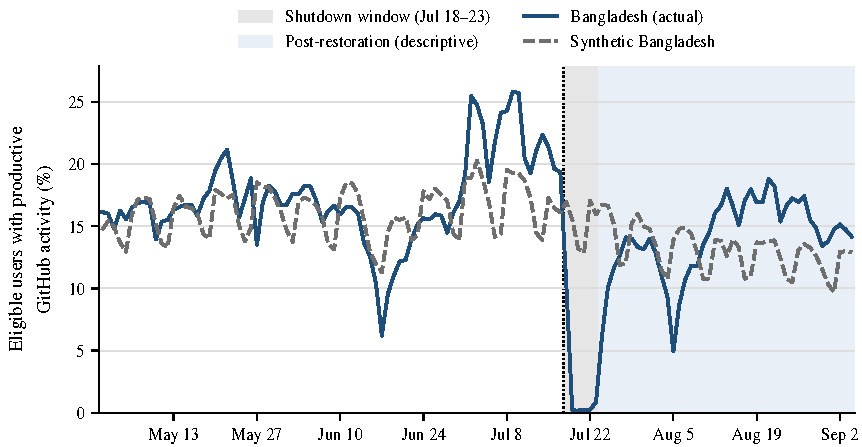
\includegraphics[width=\textwidth]{fig1_sc_actual_vs_synthetic.pdf}
\fignote{The solid line is the daily percentage of eligible Bangladesh-associated GitHub accounts with observable productive GitHub activity; the dashed line is the synthetic control, a weighted combination of Pakistan (47.6\%), Ghana (32.5\%), and Kenya (19.9\%) with weights chosen on May 1--July 17, 2024 (\cref{tab:sc_main}). The shaded shutdown interval defines the primary treatment estimand. Post-restoration differences are shown descriptively and are not interpreted as additional causal treatment effects. The grey band marks the July 18--23 shutdown and the dotted line its onset; the blue band marks the post-restoration period, July 24--September 4, over which the synthetic series is extended with the same weights. Average weekly gaps in weeks $+4$ and $+5$ after the shutdown (4.24 and 4.67 percentage points) remain within the range of pre-treatment weekly gaps ($-$2.86 to 5.88 percentage points). The dips on June 17 and August 5 coincide with national holidays coded in the country-day panel. Pre-treatment fit is imperfect (pre-treatment RMSPE 3.26 percentage points), most visibly in early July, when Bangladesh lies above its synthetic counterpart. The outcome measures observable public GitHub activity, not total software productivity. Sources: \texttt{results/synthetic\_control/actual\_vs\_synthetic\_daily.csv} (through July 23); \texttt{results/synthetic\_control/reproduced/sc\_daily\_path\_full.csv} and \texttt{sc\_weekly\_gaps.csv}, computed by \texttt{analysis/synthetic\_control/01\_reproduce\_sc.py}, which reproduces the archived weights and daily series exactly.}
\end{figure}

% Generated by analysis/tables/make_all_tables.py -- do not edit by hand.
\begin{table}[htbp]
\centering
\small
\caption{Synthetic control: main estimates and placebo inference}
\label{tab:sc_main}
\begin{threeparttable}
\begin{tabular*}{0.72\textwidth}{@{\extracolsep{\fill}}lr}
\toprule
Statistic & Value \\
\midrule
\multicolumn{2}{l}{\textit{A. Estimates, July 18--23, 2024}} \\
Bangladesh, actual (\%) & 2.021 \\
Synthetic counterfactual (\%) & 15.277 \\
ATT (percentage points) & $-$13.256 \\
Relative effect & $-$86.8\% \\
\addlinespace \multicolumn{2}{l}{\textit{B. Fit and in-space placebo inference}} \\
Pre-treatment RMSPE (pp) & 3.260 \\
Post-treatment RMSPE (pp) & 13.666 \\
Post/pre RMSPE ratio & 4.192 \\
Placebo countries & 14 \\
Rank $p$-value, absolute ATT & 0.0667 \\
Rank $p$-value, RMSPE ratio & 0.0667 \\
\addlinespace \multicolumn{2}{l}{\textit{C. Donor weights}} \\
Pakistan & 47.6\% \\
Ghana & 32.5\% \\
Kenya & 19.9\% \\
\bottomrule
\end{tabular*}
\begin{tablenotes}[flushleft]
\footnotesize\raggedright
\item \textit{Notes:} Outcome: daily percentage of eligible users with observable productive GitHub activity. Weights are chosen on May 1--July 17, 2024; the other eleven donors receive zero weight. Rank $p$-values compare Bangladesh with 14 in-space placebos; $1/15=0.0667$ is the minimum attainable value, so it indicates that Bangladesh is the most extreme unit, not $p<0.05$. Full placebo ranking in \cref{tab:sc_placebos}. Sources: \texttt{results/synthetic\_control/sc\_inspace\_placebos.csv}, \texttt{results/final/table\_primary\_SC\_weights.csv}.
\end{tablenotes}
\end{threeparttable}
\end{table}


The synthetic control places 47.6 percent weight on Pakistan, 32.5 percent on Ghana, and 19.9 percent on Kenya (\cref{tab:sc_main}). No other donor receives positive weight in the baseline optimization. After restoration, shown descriptively in \cref{fig:sc}, the average weekly gap between Bangladesh and its synthetic counterpart narrows to about $-$3 percentage points in the first two weeks ($-$3.11 and $-$2.89 percentage points) and turns positive in the third week; the positive average gaps in weeks $+4$ and $+5$ (4.24 and 4.67 percentage points) lie within the range of pre-treatment weekly gaps and are not interpreted as effects of the shutdown or of restoration. Bangladesh is more extreme than all fourteen in-space placebos in both absolute ATT and RMSPE-ratio comparisons, yielding rank statistics of 0.0667, the smallest value attainable with fourteen placebo units (\cref{fig:placebo,tab:sc_placebos}).

\begin{figure}[htbp]
\centering
\caption{Synthetic-control in-space placebo inference: post/pre-treatment RMSPE ratios}
\label{fig:placebo}
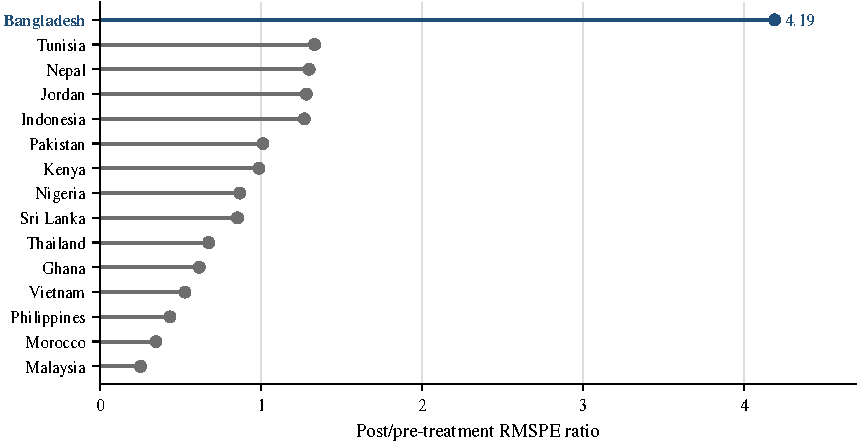
\includegraphics[width=\textwidth]{fig2_sc_placebo_rmspe_ratio.pdf}
\fignote{Each donor country is assigned the July 18--23 treatment in turn, and its synthetic control is rebuilt from the remaining donors. The figure ranks Bangladesh and the 14 placebo countries by the ratio of post-treatment to pre-treatment RMSPE, a statistic that scales the treatment-period gap by each unit's pre-treatment fit. Bangladesh is the most extreme of the 15 units; it also has the largest absolute ATT. The exact rank $p$-value is therefore $1/15 = 0.0667$ for both statistics. This is the minimum attainable value with 14 placebo countries: Bangladesh is the most extreme unit in the placebo distribution, but the resolution of exact placebo inference is limited by the size of the donor pool. Source: \texttt{results/synthetic\_control/sc\_inspace\_placebos.csv}, verified against \texttt{results/final/table\_primary\_SC\_placebos.csv}.}
\end{figure}

The leave-one-out exercise is highly stable (\cref{tab:loo} in \cref{sec:sc_diagnostics}). Across specifications that remove one donor at a time, the ATT ranges only from $-$13.256 to $-$12.886 percentage points. In particular, excluding Pakistan produces $-$12.905 percentage points, excluding Ghana produces $-$13.209 percentage points, and excluding Kenya produces $-$12.886 percentage points. This matters because both Pakistan and Kenya experienced localized connectivity disruptions near the broader pre-treatment period: Internet Society reports regional restrictions in Pakistan around July 14--17, while Cloudflare documents a major Kenyan traffic disruption on June 25 \citep{isoc2024,cloudflare2024}.
% TODO: REPLACE BANGLADESH INTERNET SOCIETY ENTRY WITH PAKISTAN-SPECIFIC SOURCE
The limited movement in the treatment estimate when either donor is removed reduces, though does not eliminate, concern that these donor-specific episodes drive the result.

\subsection{Difference-in-differences and event study}
\label{sec:did_results}

The international DiD estimate is $-$13.088 percentage points, nearly identical to the synthetic-control ATT (\cref{tab:did}, Panel A). Removing national holidays yields $-$13.379 percentage points. The agreement is notable because the two methods use different weighting logic: synthetic control chooses donor weights to reproduce Bangladesh before the shutdown, whereas the international DiD gives equal weight to donor-country changes. Bangladesh's estimate is also more extreme than that of every in-space placebo, whose estimates range from $-$1.72 to 1.60 percentage points; as for the synthetic control, the resulting rank value of 0.0667 is the minimum attainable with fifteen countries.

% Generated by analysis/tables/make_all_tables.py -- do not edit by hand.
\begin{table}[htbp]
\centering
\footnotesize
\caption{International difference-in-differences and aggregate event study}
\label{tab:did}
\begin{threeparttable}
\begin{tabular}{lrrrrrrr}
\toprule
& BD pre & BD shut- & Donor & ATT & Relative & Placebo & Rank \\
Specification & (\%) & down (\%) & change & (pp) & effect & SD & $p$ \\
\midrule
\multicolumn{8}{l}{\textit{A. Difference-in-differences, July 18--23 vs.\ May 1--July 17}} \\
All days & 17.25 & 2.02 & $-$2.15 & $-$13.09 & $-$86.6\% & 1.17 & 0.0667 \\
Holidays excluded & 17.58 & 2.02 & $-$2.18 & $-$13.38 & $-$86.9\% & 1.19 & 0.0667 \\
\addlinespace \multicolumn{8}{l}{\textit{B. Event study, selected weeks (all weeks in \cref{tab:did_es_full})}} \\
\multicolumn{4}{l}{Event week (dates)} & $\hat\theta_k$ (pp) & Placebo-based interval & Placebo SD & Rank $p$ \\
\multicolumn{4}{l}{$-5$ (Jun 13--Jun 19)} & $-$4.89 & [$-$9.31, $-$0.47] & 2.26 & 0.0667 \\
\multicolumn{4}{l}{$-2$ (Jul 4--Jul 10)} & 6.10 & [3.76, 8.43] & 1.19 & 0.0667 \\
\multicolumn{4}{l}{$-1$ (Jul 11--Jul 17)} & 3.86 & [2.15, 5.58] & 0.88 & 0.0667 \\
\multicolumn{4}{l}{$0$ (Jul 18--Jul 23)} & $-$13.09 & [$-$15.39, $-$10.79] & 1.17 & 0.0667 \\
\multicolumn{4}{l}{$+1$ (Jul 24--Jul 30)} & $-$2.66 & [$-$5.35, 0.02] & 1.37 & 0.0667 \\
\multicolumn{4}{l}{$+2$ (Jul 31--Aug 6)} & $-$2.76 & [$-$4.87, $-$0.65] & 1.08 & 0.0667 \\
\multicolumn{4}{l}{$+3$ (Aug 7--Aug 13)} & 0.52 & [$-$1.99, 3.02] & 1.28 & 0.9333 \\
\multicolumn{4}{l}{$+4$ (Aug 14--Aug 20)} & 4.31 & [1.99, 6.64] & 1.18 & 0.0667 \\
\multicolumn{4}{l}{$+5$ (Aug 21--Aug 27)} & 4.84 & [2.40, 7.28] & 1.24 & 0.0667 \\
\multicolumn{4}{l}{$+6$ (Aug 28--Sep 3)} & 2.53 & [0.01, 5.05] & 1.29 & 0.0667 \\
\bottomrule
\end{tabular}
\begin{tablenotes}[flushleft]
\footnotesize\raggedright
\item \textit{Notes:} Outcome: daily percentage of eligible users with observable productive GitHub activity. Panel A compares Bangladesh's change from May 1--July 17 to July 18--23 with the equal-weighted mean change of the 14 donor countries (\cref{eq:did_agg}); the ATT reproduces \texttt{results/final/table\_DiD\_all\_outcomes.csv}. Panel B reports $\hat\theta_k$ (\cref{eq:es_agg}) for weekly bins; week 0 equals the Panel A all-days ATT. Weeks $-5$ and $-2$ are the most negative and most positive pre-shutdown estimates. Inference uses in-space placebos: each donor is compared in turn with the mean of the other 13. \textit{Placebo SD}: standard deviation of the 14 placebo estimates. \textit{Placebo-based interval}: $\hat\theta_k\pm1.96\times$SD, a donor-placebo reference interval, not a conventional sampling confidence interval. \textit{Rank $p$}: share of the 15 units whose absolute estimate is at least as large as Bangladesh's (minimum 0.0667). Bangladesh's pre-period weekly estimates are more volatile than any donor's, so these placebo-based measures are not fully calibrated sampling uncertainty for Bangladesh. The pre-period does not show a clean parallel-trends pattern, and the weekly coefficients are a diagnostic, not an identified dynamic treatment path; the synthetic control remains the main design. Sources: \texttt{results/did/did\_main\_placebo\_inference.csv}, \texttt{results/did/did\_eventstudy\_weekly.csv}.
\end{tablenotes}
\end{threeparttable}
\end{table}


\Cref{fig:did_es} reports the weekly event study from \cref{eq:es_agg}. Its shutdown-week coefficient, $-$13.09 percentage points, reproduces the aggregate DiD estimate and is more than twice as large in absolute value as any pre-shutdown weekly coefficient. The pre-shutdown period, however, is volatile and does not display a clean conventional parallel-trends pattern. Weekly coefficients range from $-$4.89 percentage points (week $-5$, June 13--19) to 6.10 (week $-2$, July 4--10), and Bangladesh was above its pre-period position relative to the donors in the two weeks immediately before the shutdown. This mirrors the imperfect early-July fit of the synthetic control (\cref{fig:sc}). Because the reference is the full pre-period mean, this elevated activity does not generate the shutdown estimate; measured against the immediately preceding week alone, the decline would be larger. Given this pre-period volatility, the weekly coefficients are not interpreted as an identified dynamic causal treatment path. They are diagnostic evidence that the largest break in the series is concentrated in the shutdown week.

\begin{figure}[htbp]
\centering
\caption{Diagnostic event study: Bangladesh relative to the equal-weighted donor mean, by week}
\label{fig:did_es}
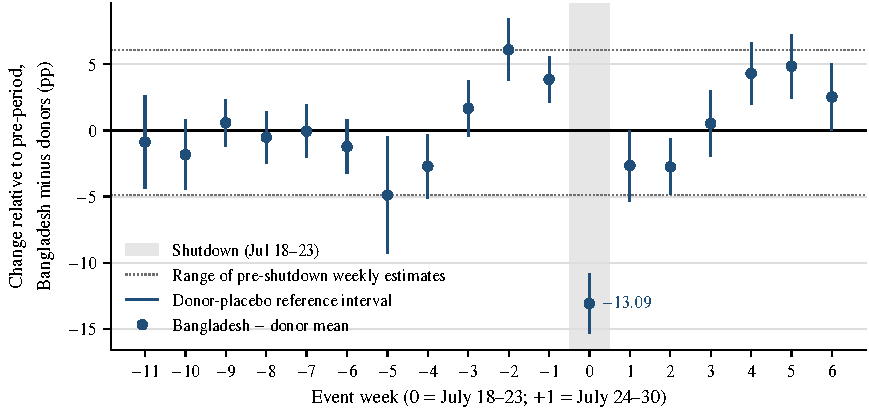
\includegraphics[width=\textwidth]{fig3_did_eventstudy.pdf}
\fignote{Points are $\hat\theta_k$ from \cref{eq:es_agg}: the change in Bangladesh's daily percentage of eligible users with observable productive GitHub activity, relative to its May 1--July 17 mean, minus the corresponding change averaged over the 14 donor countries with equal weights. Week 0 is the July 18--23 shutdown (shaded); its coefficient equals the DiD estimate in \cref{tab:did}. Weeks $-11$ to $-1$ are seven-day bins ending July 17 (week $-11$ includes May 1); weeks $+1$ to $+6$ are seven-day bins from July 24 to September 3. Vertical lines are donor-placebo reference intervals, $\hat\theta_k \pm 1.96$ times the standard deviation of the 14 in-space placebo estimates for the same week; they are not conventional sampling confidence intervals. Dotted horizontal lines mark the minimum and maximum of Bangladesh's pre-shutdown weekly coefficients. Bangladesh's pre-period estimates are more volatile than those of any donor country, so the reference intervals should not be interpreted as fully calibrated sampling uncertainty. The pre-period does not show a clean parallel-trends pattern; the coefficients are a diagnostic complement to the synthetic control, not an identified dynamic treatment path. Source: \texttt{results/did/did\_eventstudy\_weekly.csv} (script \texttt{analysis/did/01\_aggregate\_did\_eventstudy.py}, input \texttt{results/synthetic\_control/country\_day\_donor\_pool\_with\_holidays.parquet}). Week 0 is verified against \texttt{results/final/table\_DiD\_all\_outcomes.csv}.}
\end{figure}

The donor-placebo reference intervals in \cref{fig:did_es} should be read with care. They are not conventional sampling confidence intervals: they scale the spread of the fourteen donor placebo estimates in each week. Bangladesh's pre-shutdown weekly coefficients have a standard deviation of 3.04 percentage points, compared with 0.70 to 2.18 percentage points for the donors treated as placebo units. Several pre-period coefficients for Bangladesh are therefore as extreme as any placebo, and the reference intervals are not fully calibrated measures of uncertainty for Bangladesh. The more informative comparison is with Bangladesh's own pre-shutdown range: the shutdown coefficient lies far outside it, whereas every post-restoration coefficient lies within it.

After restoration, the gap narrows quickly. The coefficients are $-$2.66 and $-$2.76 percentage points in the two weeks after the shutdown and are positive from week $+3$ onward. The positive coefficients in weeks $+4$ to $+6$ (2.53 to 4.84 percentage points) lie within the range of pre-shutdown fluctuations and should not be interpreted as gains caused by the shutdown. User-day event-study estimates from earlier auxiliary analyses are not reported because their implementation is not fully documented. Recovery dynamics within Bangladesh are examined by repository sector in \cref{sec:sector_results}.

\subsection{Regression discontinuity in time}
\label{sec:rdit_results}

\Cref{fig:rdit} shows the daily series used in the RDiT. In Bangladesh, the share of users with productive activity is 19.03 percent on July 17, falls to 10.74 percent on July 18, and lies between 0.48 and 1.23 percent from July 19 through July 23 before recovering gradually from July 24. The Philippines, used as a geographic placebo, shows no comparable break.

\begin{figure}[htbp]
\centering
\caption{Regression discontinuity in time: daily share of users with productive activity around the July 17 cutoff (visual companion to \cref{tab:rdit})}
\label{fig:rdit}
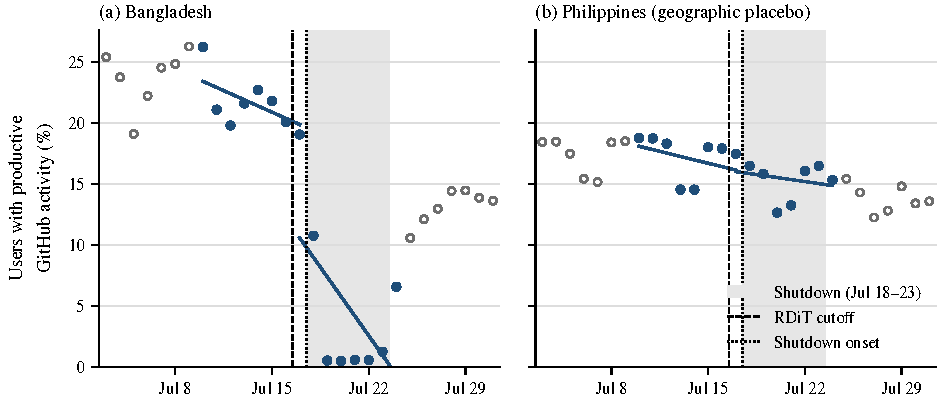
\includegraphics[width=\textwidth]{fig7_rdit_cutoff.pdf}
\fignote{Daily percentage of users with at least one productive GitHub event in the balanced user-day panels used for the RDiT (10,329 Bangladesh-associated and 3,025 Philippines-associated accounts), July 3--31, 2024. Filled markers are the fifteen days inside the 7-day bandwidth of \cref{eq:rdit} (July 10--24); hollow markers are shown for context. Lines are the local linear fits of the archived preferred specification on each side of the cutoff; the dashed vertical line marks the RDiT cutoff, with July 17 ($\tilde t=0$) on the post-cutoff side, and the dotted vertical line marks the shutdown boundary between July 17 and July 18. The shaded band is the July 18--23 shutdown. The figure is a visual companion to the formal estimates in \cref{tab:rdit}; the fitted lines correspond exactly to those estimates. Source: \texttt{results/rdit/rdit\_daily\_series.csv}, written by \texttt{analysis/rdit/01\_reproduce\_rdit.py} from \texttt{data/processed/panel\_user\_day\_bangladesh.parquet} and \texttt{panel\_user\_day\_philippines.parquet}; the same script reproduces the archived estimates in \texttt{results/rdit/main\_rdit\_summary.csv} exactly.}
\end{figure}

The RDiT produces a smaller point estimate but the same qualitative conclusion (\cref{tab:rdit}). The preferred local linear specification estimates a discontinuity of $-$9.28 percentage points in Bangladesh's active-user rate; a controlled Bangladesh-minus-Philippines version yields $-$9.16 percentage points. HAC $p$-values are approximately 0.065 in both cases, while the Philippines placebo is near zero. The smaller magnitude than in the synthetic control and DiD is consistent with the design visible in \cref{fig:rdit}: the cutoff day, July 17, precedes the shutdown but lies on the post-cutoff side, and the linear post-cutoff fit spans both the collapse and the beginning of the recovery on July 24.
Consistent with \citet{hausman2018}, I therefore emphasize the direction and timing of the break rather than treating the RDiT $p$-value as the decisive inferential statistic.

% Generated by analysis/tables/make_all_tables.py -- do not edit by hand.
\begin{table}[H]
\centering
\footnotesize
\caption{Regression discontinuity in time: preferred specification}
\label{tab:rdit}
\begin{threeparttable}
\begin{tabular}{l>{\raggedright\arraybackslash}p{3.3cm}rrcrr}
\toprule
Specification & Outcome & Effect (pp) & HAC SE & 95\% CI & $p$ & Days \\
\midrule
Main local linear & Bangladesh active rate & $-$9.284 & 5.034 & [$-$19.151, 0.584] & 0.065 & 15 \\
Controlled local linear & Bangladesh $-$ Philippines active rate & $-$9.160 & 4.980 & [$-$18.921, 0.601] & 0.066 & 15 \\
Geographic placebo & Philippines active rate & $-$0.124 & 1.492 & [$-$3.048, 2.801] & 0.934 & 15 \\
\bottomrule
\end{tabular}
\begin{tablenotes}[flushleft]
\footnotesize\raggedright
\item \textit{Notes:} Local linear RDiT at the July 17, 2024 cutoff, bandwidth 7 days, polynomial degree 1, no donut, HAC lags 2. Effects are reported in percentage points. RDiT is a temporal robustness check, not the primary causal design. Source: \texttt{results/rdit/main\_rdit\_summary.csv}.
\end{tablenotes}
\end{threeparttable}
\end{table}


\subsection{Productive, shipping, and collaboration outcomes}
\label{sec:secondary}

The collapse is not limited to a generic activity indicator. Holding the primary synthetic-control weights fixed, productive activity falls by 15.179 percentage points relative to a 17.555 percent counterfactual, or 86.5 percent. Shipping activity falls by 1.333 percentage points relative to a 1.415 percent counterfactual, or 94.2 percent. Collaboration activity falls by 0.780 percentage points relative to a 0.834 percent counterfactual, or 93.6 percent. Count outcomes show similarly large relative declines in collaboration events and shipping output (\cref{tab:secondary}). International DiD estimates for the same outcomes, which point in the same direction, are reported in \cref{tab:did_secondary}.

Allowing the donor weights to re-optimize separately for each outcome produces comparable magnitudes: $-$86.2 percent for productive activity, $-$92.2 percent for shipping activity, and $-$92.1 percent for collaboration activity. The in-space placebo ATT rank is again 0.0667 for all three key activity-rate outcomes. The RMSPE-ratio rank is 0.0667 for productive and shipping activity but 0.20 for collaboration activity. I therefore treat collaboration as consistent secondary evidence rather than giving it the same inferential weight as the primary and shipping outcomes.

% Generated by analysis/tables/make_all_tables.py -- do not edit by hand.
\begin{table}[htbp]
\centering
\footnotesize
\caption{Secondary outcomes}
\label{tab:secondary}
\begin{threeparttable}
\begin{tabular}{lrrrrrr}
\toprule
 & \multicolumn{2}{c}{Fixed primary weights} & \multicolumn{2}{c}{Outcome-specific weights} & \multicolumn{2}{c}{Placebo rank} \\ \cmidrule(lr){2-3}\cmidrule(lr){4-5}\cmidrule(lr){6-7}
Outcome & ATT & Relative & ATT & Relative & ATT & RMSPE ratio \\
\midrule
Productive active rate & $-$15.179 pp & $-$86.5\% & $-$14.870 pp & $-$86.2\% & 0.0667 & 0.0667 \\
Shipping active rate & $-$1.333 pp & $-$94.2\% & $-$0.964 pp & $-$92.2\% & 0.0667 & 0.0667 \\
Collaboration active rate & $-$0.780 pp & $-$93.6\% & $-$0.630 pp & $-$92.1\% & 0.0667 & 0.2000 \\
Collaboration events / 1,000 & $-$24.095 & $-$95.1\% & $-$18.589 & $-$93.7\% & -- & -- \\
Shipping output / 1,000 & $-$23.981 & $-$93.9\% & $-$18.192 & $-$92.1\% & -- & -- \\
\bottomrule
\end{tabular}
\begin{tablenotes}[flushleft]
\footnotesize\raggedright
\item \textit{Notes:} Fixed-weight specifications reuse the primary active-rate SCM weights (\cref{tab:weights}). Outcome-specific specifications re-estimate donor weights separately for each outcome (\cref{tab:weights_specific}). Rank values are exact in-space placebo ranks for the outcome-specific specifications with 14 placebo countries; 0.0667 is the minimum attainable value. Placebo ranks are not reported for the count outcomes.
\end{tablenotes}
\end{threeparttable}
\end{table}


\subsection{Sectoral recovery after restoration}
\label{sec:sector_results}

The synthetic-control estimates describe the collapse during the shutdown window. They do not show how activity evolved once connectivity returned, or whether recovery was common across the kinds of projects on which Bangladeshi developers work. This subsection addresses these questions using the fixed sample of 20,000 Bangladesh-associated accounts and the repository-sector classification of \cref{sec:sector_data}, estimated as described in \cref{sec:sector_method}. The analysis compares each sector with its own pre-shutdown baseline. It documents heterogeneity in recovery dynamics within Bangladesh; it does not estimate sector-specific causal effects relative to an untreated international control, and the synthetic-control estimate in \cref{sec:main_results} remains the paper's headline result. Throughout, a sector refers to the economic sector associated with the repositories in which observable GitHub activity occurs, not to developers' employers or industries of employment.

% Generated by analysis/tables/make_all_tables.py -- do not edit by hand.
\begin{table}[htbp]
\centering
\footnotesize
\caption{Recovery of observable GitHub push activity by repository sector}
\label{tab:sector_recovery}
\begin{threeparttable}
\begin{tabular}{lrrrrrrrrr}
\toprule
& & Pre & Pre rate & \multicolumn{5}{c}{Recovery index (pre-period mean = 100)} & First wk \\
\cmidrule(lr){5-9}
Sector & NAICS & users & (\%) & Shutdown & +1 & +2 & +4 & +8 & $\geq$80, 2 wks \\
\midrule
Finance & 52 & 382 & 0.078 & 30.9 & 92.2 & 67.6 & 89.5 & 91.3 & 3 \\
Information & 51 & 1,528 & 0.442 & 11.7 & 75.9 & 72.2 & 106.0 & 94.5 & 3 \\
Education & 61 & 1,234 & 0.385 & 11.7 & 59.1 & 53.4 & 75.4 & 81.9 & 6 \\
Health & 62 & 514 & 0.132 & 6.3 & 40.7 & 51.5 & 77.5 & 89.4 & 6 \\
Retail & 44--45 & 1,012 & 0.295 & 6.2 & 52.0 & 52.3 & 153.7 & 79.6 & 9 \\
Real Estate & 53 & 213 & 0.063 & 4.0 & 33.0 & 25.1 & 44.4 & 85.5 & 5 \\
Accommodation/Food & 72 & 480 & 0.144 & 3.5 & 44.3 & 42.8 & 54.2 & 62.6 & -- \\
\bottomrule
\end{tabular}
\begin{tablenotes}[flushleft]
\footnotesize\raggedright
\item \textit{Notes:} Fixed sample of 20,000 Bangladesh-associated accounts. Repository sectors from the historical-README classifier with confidence $\geq$ 0.80. The outcome is the share of sampled users with at least one PushEvent to a repository of the sector on a given day. \textit{Pre users}: sampled users with such activity in the baseline period. \textit{Pre rate}: mean daily outcome over the baseline period (May 23--July 17, 2024, the final eight complete pre-shutdown weeks), in percent of all 20,000 users. Shutdown: July 18--23; week +1: July 24--30; subsequent 7-day bins. \textit{First wk $\geq$80, 2 wks}: first post-shutdown week that begins two consecutive weeks with an index of at least 80 (observed through week +17, November 13--19); it does not imply that the index stays above 80 thereafter. -- indicates no such week. Within-Bangladesh comparison with the sector's own pre-period; not a causal effect relative to an untreated control. Sources: \texttt{results/sector\_recovery/sectorwide/sectorwide\_recovery\_summary.csv}, verified against \texttt{results/sector\_recovery/final/table\_sector\_recovery\_main.csv}.
\end{tablenotes}
\end{threeparttable}
\end{table}


All seven sectors show a sharp fall in observable push activity during July 18--23 (\cref{tab:sector_recovery,fig:sector_index}). The shutdown-period recovery index ranges from 3.5 in Accommodation/Food to 11.7 in Information and Education and 30.9 in Finance. In every sector, the 95 percent confidence interval for the change relative to the baseline excludes zero (\cref{fig:sector_es}).

Restoration of connectivity did not imply an immediate or uniform recovery. In the first week after the shutdown (July 24--30), the recovery index ranges from 33.0 in Real Estate to 92.2 in Finance. Mobile connectivity returned only during this week, later than fixed broadband \citep{belson2024}, so part of the week $+1$ shortfall may reflect incomplete restoration. Recovery was also not monotonic: in Finance, Information, Education, Real Estate, and Accommodation/Food, the index is lower in week $+2$ (July 31--August 6) than in week $+1$. The data do not identify the source of this second-week decline.

\begin{figure}[htbp]
\centering
\caption{Recovery of observable GitHub push activity by repository sector}
\label{fig:sector_index}
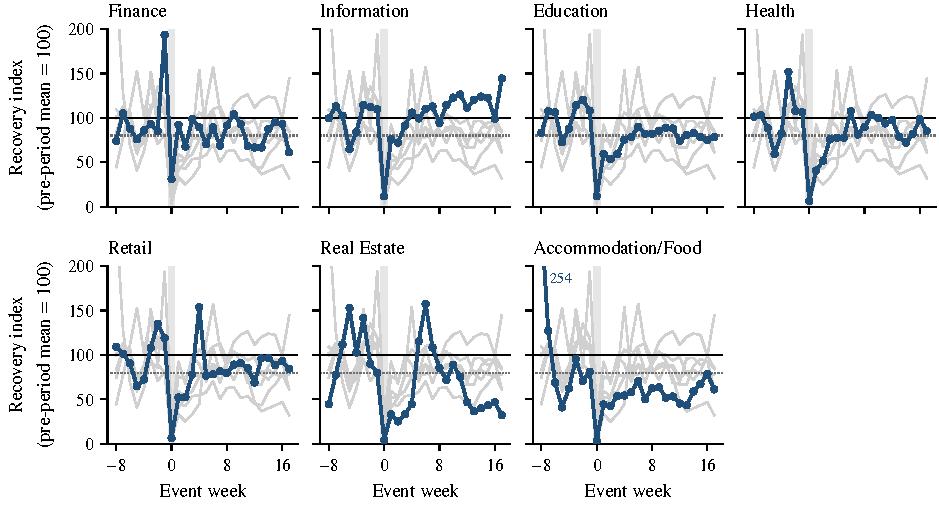
\includegraphics[width=\textwidth]{fig5_sector_recovery_index.pdf}
\fignote{Each panel highlights one sector's recovery index $R_{sk}$ (\cref{eq:sector}); the other six sectors are shown in light grey for comparison. The index is 100 times the sector's mean daily probability of push activity in event week $k$, divided by its mean over the final eight complete pre-shutdown weeks (May 23--July 17, 2024). The shaded band is the July 18--23 shutdown ($k=0$); week $+1$ is July 24--30, followed by consecutive seven-day bins. Solid and dotted horizontal lines mark 100 and 80. The common vertical axis is truncated at 200; the one value above it (Accommodation/Food, week $-8$) is labeled. Fixed sample of 20,000 Bangladesh-associated accounts; repository sectors from the historical-README classifier with confidence $\geq 0.80$. The sector is that of the repositories in which activity occurs, not the developer's employer. Within-Bangladesh comparison with each sector's own baseline; not a causal effect relative to an untreated control. Source: \texttt{results/sector\_recovery/sectorwide/sectorwide\_user\_eventstudy.csv}, verified against \texttt{results/sector\_recovery/final/table\_sector\_recovery\_main.csv}.}
\end{figure}

Finance and Information recovered fastest. Finance returned to an index of 92.2 in week $+1$, and both sectors begin a run of two consecutive weeks at or above 80 in week $+3$. Information exceeds its baseline by week $+4$ (106.0). In week $+8$, the two indices are 94.5 and 91.3. The Finance series is nonetheless noisy: its baseline includes a spike in week $-1$ (index 193.6), and its post-shutdown index falls back below 80 in several later weeks.

Education and Health recovered more gradually. Their week $+1$ indices are 59.1 and 40.7, they reach 75.4 and 77.5 by week $+4$, and both begin a run of two consecutive weeks at or above 80 only in week $+6$. By week $+8$, they stand at 81.9 and 89.4.

Accommodation/Food remained persistently depressed. Its index is 44.3 in week $+1$, 54.2 in week $+4$, and 62.6 in week $+8$, and it never records two consecutive weeks at or above 80 through the end of the observation window (week $+17$, November 13--19). This result should be read alongside the sector's unstable baseline: the index is 254.1 and 127.3 in the first two baseline weeks and between 40.8 and 95.5 in the remaining six. Part of the post-shutdown gap may therefore reflect a decline that began before the shutdown rather than a failure to recover.

Real Estate recovered slowly at first and later approached its baseline. Its index remains between 25.1 and 44.4 through week $+4$, rises above 100 in weeks $+5$ and $+6$ (115.1 and 157.3), and is 85.5 in week $+8$. This later recovery is not durable within the observed window: from week $+12$ onward, the index lies between 31.9 and 46.7 (\cref{fig:sector_es}). Real Estate is also the smallest of the seven sectors, with 213 sampled users active in the baseline period, so its weekly estimates are imprecise.

Retail shows a pronounced temporary rebound. Its index is about 52 in weeks $+1$ and $+2$, rises to 153.7 in week $+4$ (August 14--20), and falls back to 76.5 in week $+5$. Its first run of two consecutive weeks at or above 80 begins only in week $+9$. The week $+4$ value is therefore a transient overshoot, possibly reflecting a burst of catch-up activity, rather than evidence of completed recovery; the data do not identify what generated it. The timing of Retail's first sustained run is also sensitive to the classifier threshold (\cref{sec:sector_robustness}).

Index values above 100 later in the window should not be read as gains caused by the shutdown. Information, for example, has an index between 111.5 and 126.4 in weeks $+10$ to $+15$ and 144.3 in week $+17$. Without an untreated comparison group, such movements cannot be separated from trend growth, seasonality, or changes in the sampled users' activity.

\begin{figure}[htbp]
\centering
\caption{Sectoral event study: change in daily push-activity probability relative to the pre-shutdown baseline}
\label{fig:sector_es}
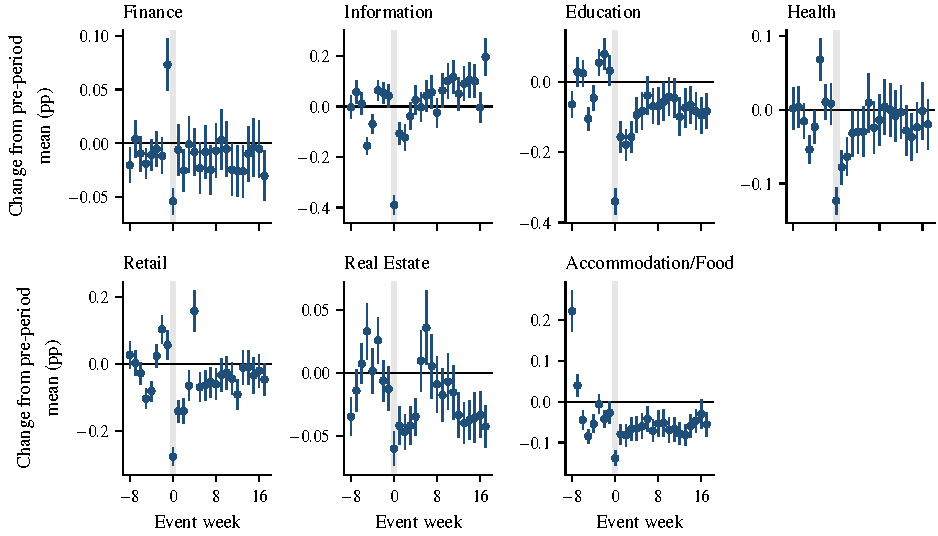
\includegraphics[width=\textwidth]{fig6_sector_eventstudy.pdf}
\fignote{Points are $\beta_{sk}$ from \cref{eq:sector}: the mean change, across the fixed sample of 20,000 Bangladesh-associated accounts, in the daily probability of a PushEvent in a sector-$s$ repository during event week $k$, relative to each user's mean over the final eight complete pre-shutdown weeks, in percentage points. Vertical lines are 95 percent confidence intervals based on the cross-user standard deviation of these differences; they do not account for common weekly shocks. The shaded band is the July 18--23 shutdown ($k=0$); week $+1$ is July 24--30, and the window extends to week $+17$ (November 13--19, 2024). Vertical scales differ across panels because baseline activity levels differ by sector (\cref{tab:sector_recovery}). Repository sectors from the historical-README classifier with confidence $\geq 0.80$. Within-Bangladesh comparison; not a causal effect relative to an untreated control. Source: \texttt{results/sector\_recovery/sectorwide/sectorwide\_user\_eventstudy.csv}.}
\end{figure}

The main specification counts pushes to any classified repository, including repositories first observed after the shutdown. A complementary specification follows only repositories pushed to during the eight baseline weeks (\cref{tab:sector_fixed_repo}). Activity in these pre-existing repositories recovers far less: in week $+8$, their indices range from 10.1 (Accommodation/Food) to 31.4 (Education), compared with 62.6 to 94.5 in the sector-wide specification. Because repositories selected on recent activity would become less active over time even without a shutdown, this gap does not measure a shutdown effect. It is nevertheless consistent with recovery occurring partly through new repositories and switching across projects rather than solely through a return to pre-existing ones.

Taken together, the sectoral evidence indicates that the collapse in observable activity documented in \cref{sec:main_results} was followed by a recovery that was gradual and uneven across the economic sectors associated with developers' repositories. These are before--after comparisons within Bangladesh. They share the identification limitations discussed in \cref{sec:unrest} and, in addition, cannot separate post-shutdown recovery from other Bangladesh-specific developments between August and November 2024.

\section{Mechanism: Offline Work and Delayed Synchronization}
\label{sec:mechanism}

\subsection{Main backlog measure}
\label{sec:backlog}

A fall in public GitHub events does not necessarily imply an equal fall in code creation. Git is decentralized: developers may continue editing files and creating commits locally, then push them only after connectivity returns. The commit-level analysis directly tests for this pattern.

In the strict sample, 2,932 commits are authored during July 18--23. Of these, 829 first appear in a public push on or after July 24. The resulting author-time backlog share is 28.27 percent (\cref{tab:mechanism}). Replacing the author timestamp with the committer timestamp produces a nearly identical 27.16 percent backlog share (790 of 2,909 commits). The agreement between the two metadata clocks is useful because neither timestamp is a perfect external record of when coding occurred. Both timestamps are Git metadata generated by the author's local client or the hosting platform at commit time, not an externally verified record of the exact physical moment the code was written; the mechanism evidence is therefore consistent with offline or local work followed by delayed synchronization, but it does not directly observe the underlying production process.

Long publication delays become dramatically more common during the shutdown. Among shutdown-authored commits, 29.71 percent have an author-to-push delay above 24 hours, 25.38 percent above 48 hours, and 22.75 percent above 72 hours. In six overlapping pre-shutdown placebo windows, the corresponding averages are approximately 1.10 percent, 0.72 percent, and 0.46 percent (\cref{tab:mech_placebos}). Because commit metadata were queried for only a daily sample of commits pushed before July 18 but for all commits pushed from July 18 onward, the placebo rates use inverse-probability weights, while shutdown-authored commits, all pushed on or after July 18, receive weight one. The real shutdown is therefore far outside the normal pre-period delay distribution.

% Generated by analysis/tables/make_all_tables.py -- do not edit by hand.
\begin{table}[htbp]
\centering
\footnotesize
\caption{Commit-time mechanism}
\label{tab:mechanism}
\begin{threeparttable}
\begin{tabular}{lrrrrrrr}
\toprule
Timestamp & $N$ during & Pushed & Backlog & $>$24h & $>$48h & $>$72h & Mean \\
 & shutdown & Jul 24+ & share & & & & delay (h) \\
\midrule
\texttt{authoredDate} & 2,932 & 829 & 28.27\% & 29.71\% & 25.38\% & 22.75\% & 40.94 \\
\texttt{committedDate} & 2,909 & 790 & 27.16\% & 28.60\% & 24.27\% & 21.73\% & 37.47 \\
\bottomrule
\end{tabular}
\begin{tablenotes}[flushleft]
\footnotesize\raggedright
\item \textit{Notes:} Strict sample requires author login = PushEvent actor, a non-missing timestamp, and a nonnegative delay. The backlog share is conditional on commits observed in the mechanism sample, not a share of all software production in Bangladesh. \texttt{authoredDate} and \texttt{committedDate} are Git metadata, not externally verified measurements of when code was written.
\end{tablenotes}
\end{threeparttable}
\end{table}


\subsection{Timing and concentration of delayed pushes}
\label{sec:timing}

The delayed commits are released quickly once connectivity begins to return (\cref{fig:mechanism}). Of the 829 author-time backlog commits, 354 (42.7 percent) appear on July 24 and 544 (65.6 percent) by July 25. By July 27, 81.1 percent have appeared; by July 31, 92.0 percent have appeared. This temporal concentration immediately after restoration is consistent with a synchronization backlog rather than ordinary long-lived branches or sporadic publication.

\begin{figure}[htbp]
\centering
\caption{Release timing of commits with shutdown-period Git author timestamps}
\label{fig:mechanism}
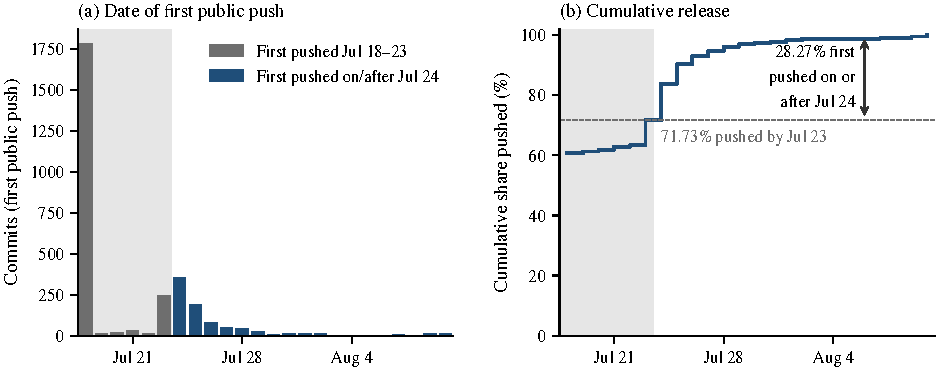
\includegraphics[width=\textwidth]{fig4_mechanism_release.pdf}
\fignote{Strict sample: commits whose GitHub-linked author equals the Bangladeshi pusher, with a non-missing author timestamp and nonnegative author-to-push delay; the cohort is the 2,932 commits authored July 18--23 (UTC). Panel (a): date of first public push; panel (b): cumulative share pushed. 829 commits (28.27\%) first appear on or after July 24; pushes are observed through August 10. Git \texttt{authoredDate} and \texttt{committedDate} are metadata, not verified measurements of when code was written; the pattern is consistent with local work followed by delayed synchronization. The share refers only to this strict sample, not to all software production in Bangladesh. Source: Author's calculations using GH Archive and GitHub commit metadata.}
\end{figure}

The backlog is not generated by only a handful of unusually active users (\cref{tab:concentration}). The 2,932 shutdown-authored commits come from 835 users and 977 repositories. Two hundred twenty-two users (26.6 percent) and 246 repositories (25.2 percent) contribute at least one backlog commit. The largest user accounts for 2.77 percent of backlog commits, the top five users for 12.06 percent, and the top ten for 21.47 percent. Dropping the twenty users with the most backlog still leaves a 20.37 percent backlog share.

Backlog is, however, more common in larger pushes (\cref{tab:push_size}). Restricting to pushes with at most 10 commits lowers the backlog share to 21.0 percent; at most 5 commits, 14.4 percent; at most 2 commits, 7.8 percent; and single-commit pushes, 3.3 percent. This pattern is economically meaningful rather than merely inconvenient: if developers accumulate local commits while offline and synchronize later, restoration should produce larger-than-normal push batches. At the same time, it means that the 28.3 percent headline mechanism estimate should not be interpreted as applying uniformly to every kind of push.

\section{Robustness, Identification Threats, and Limitations}
\label{sec:robustness}

\subsection{Synthetic-control diagnostics}
\label{sec:sc_diagnostics}

The primary synthetic control improves pre-treatment fit relative to using the Philippines alone, but the fit is not perfect. The pre-treatment RMSPE is 3.26 percentage points, and Bangladesh exhibits temporary deviations from the synthetic series in early July (\cref{fig:sc}). The paper therefore reports pre-fit explicitly rather than treating the synthetic control as a perfect replica. The unusually large post-treatment gap and the stability of the estimate under leave-one-out exercises are the main reasons the design remains informative.

The donor pool also contains countries with their own short-lived connectivity disturbances. Pakistan experienced regional restrictions around July 14--17, immediately before Bangladesh's national shutdown, and Kenya experienced a major traffic disruption on June 25. These episodes are a reason to avoid presenting donor selection as mechanically pristine. Still, removing Pakistan or Kenya individually changes the ATT by less than 0.4 percentage points. A more conservative future extension could pre-register donor exclusion rules based on third-party connectivity data and expand the donor pool to increase placebo-inference resolution.

\subsection{Metadata and measurement}
\label{sec:measurement}

Commit metadata resolution is similar across periods: 82.34 percent of the pre-period target commits are found, compared with 84.24 percent during the shutdown and 81.81 percent after (\cref{tab:metadata}). The shutdown mechanism is therefore not generated by a sharp deterioration in commit-object availability during the treatment window.

A related limitation concerns push-listing completeness: although 99.5--99.8 percent of pushes in every period expose a complete commit list, the share of nominal commits captured within complete pushes falls from 90.27 percent before the shutdown to 73.11 percent during the shutdown and 71.45 percent afterward (\cref{tab:push_completeness}). This occurs because a small number of large pushes account for a disproportionate share of commits and are more likely to have incomplete commit listings. Since the strict mechanism sample restricts to complete pushes, this does not mechanically invalidate the 28.27 percent backlog estimate, but it does imply uneven commit-level coverage across periods. The lower coverage during and after the shutdown is therefore a measurement limitation that should be considered when interpreting the mechanism results.

Location is another measurement limitation. GitHub location fields are user-entered and may be missing, stale, or imprecise. The estimates should be read as applying to accounts associated with Bangladesh and the donor countries, not as a verified census of developers physically located in each country on every date. Public-event data additionally exclude private repositories. If private and public work respond differently to a shutdown, the paper estimates the effect on the observable public margin rather than on all software production.

\subsection{Concurrent unrest and causal interpretation}
\label{sec:unrest}

The most important identification threat is that the Internet shutdown was itself a response to political unrest. Protests, curfews, transportation disruptions, workplace closures, fear, or other domestic conditions could directly reduce software work even if connectivity were available. Date fixed effects and foreign controls cannot absorb shocks unique to Bangladesh that coincide with the shutdown. For this reason, the headline estimate should be interpreted as the effect of the shutdown episode under the identifying assumption that the abrupt Bangladesh-specific deviation is primarily attributable to lost connectivity.

Several findings make the connectivity interpretation more plausible without fully proving it. First, the break is tightly aligned with the network outage. Second, activity begins to recover as connectivity returns. Third, downstream online tasks such as shipping and collaboration fall at least as strongly as the general activity rate. Fourth, commit metadata reveal a large stock of code authored during the outage but pushed immediately after restoration. A pure `developers stopped working because of unrest' story does not naturally predict that last pattern. Nevertheless, the mechanism evidence is complementary, not a substitute for randomized assignment.

\section{Discussion}
\label{sec:discussion}

The results illustrate why high-frequency digital trace data can add information beyond aggregate estimates of shutdown costs. A national GDP series cannot show whether digital workers cease production, shift to offline tasks, or accumulate work that is released later. GitHub events and metadata measure observed public activity and delayed publication; they cannot observe work that never becomes public or distinguish all unobserved adaptation from lost production.

The main estimate---an 86.8 percent decline in the daily active-user rate relative to the synthetic counterfactual (\cref{tab:sc_main})---is best interpreted as a collapse in observable online software-production activity. The mechanism shows a small observed backlog alongside a collapse in author-time levels: creation of code later observed publicly falls roughly 96--97 percent from the pre-shutdown comparison, and backlog represents about 2.5 percent of normal volume. The original 28.27 percent backlog share conditions on a much smaller calendar-cohort denominator. It does not establish that missing activity was displaced across time, or quantify destruction of work that never became public.

At the same time, delayed synchronization cannot account for the entire collapse. Most eligible users record no productive public activity during the shutdown, and the recovery backlog is much smaller than the counterfactual volume implied by the active-rate and shipping estimates. Connectivity therefore appears to matter not only for publishing already-written code but also for complementary tasks: accessing remote dependencies, coordinating with collaborators, reviewing code, resolving issues, merging pull requests, and releasing software. The especially large declines in shipping and collaboration are consistent with these channels.

The sectoral results add a dynamic dimension. In aggregate, Bangladesh's gap relative to the donor mean returned within its pre-shutdown range in the first week after restoration (\cref{fig:did_es}), but that wide and volatile range is a weak recovery criterion. The separate daily, rolling-mean and cumulative measures in Section~\ref{sec:results} give different return dates and do not show full compensation by September 4. Reconnection did not restore observable activity at once: weeks after the shutdown, activity in Education-, Health-, and especially Accommodation/Food-related repositories remained below its pre-shutdown level, while Finance- and Information-related activity recovered within about three weeks. This pattern is consistent with the costs of a shutdown extending beyond the days without connectivity and falling unevenly across types of projects. The weaker recovery of pre-existing repositories, relative to sector-wide activity, further suggests that part of the recovery took the form of new projects or switching across repositories, which an analysis restricted to pre-existing projects would miss. Because the sectoral analysis has no untreated comparison group and classifies repositories rather than workers, these interpretations remain suggestive.

The national cumulative comparison is more informative about recovery than a first return inside a wide pre-period range. Relative to the unchanged synthetic series, 8,145 active user-days are missing in the six-day shutdown window; later positive gaps partly offset, but never fully repay, the cumulative shortfall, which is 3,633 user-days at September 4. Neither this arithmetic offset nor sectoral baseline crossings identify a causal rebound. The data do not evaluate particular resilience policies, so no comparative policy recommendation is drawn.

\section{Conclusion}
\label{sec:conclusion}

Bangladesh's July 2024 Internet shutdown provides a high-frequency case study of what happens to digitally mediated production when national connectivity is abruptly removed. Using public GitHub events for 59,158 pre-active accounts across fifteen countries, the paper finds that Bangladesh's daily productive-activity rate fell by 13.26 percentage points relative to a synthetic counterfactual during July 18--23, an 86.8 percent decline. International difference-in-differences, secondary outcomes, placebos, and temporal discontinuity analyses point in the same direction (\cref{tab:main}). A diagnostic event study shows that the aggregate gap narrowed quickly after restoration, although Bangladesh's pre-shutdown weekly estimates were more volatile than those of any donor country.

The commit-level evidence shows that the observed backlog was small relative to normal creation. After the approximately 15:00 UTC July 18 onset, 1,097 commits were authored and subsequently observed publicly by August 10, a 96.35 percent fall against duration-matched pre-shutdown windows (96.75 percent against the original six-day windows). Backlog is about 2.5 percent of normal volume. The original calendar-cohort backlog share of 28.27 percent and onset-cohort share of 68.55 percent describe delayed publication among the surviving observed commits; neither establishes that total software work continued at a comparable rate.

A within-Bangladesh analysis of the restoration period adds a further qualification: reconnection did not immediately restore observable activity. Recovery was faster in Finance- and Information-related repositories than in Education- and Health-related repositories, and activity in Accommodation/Food-related repositories remained depressed throughout the observed window. These sectoral patterns are descriptive comparisons with each sector's own pre-shutdown level rather than causal estimates against an untreated control.

The paper's main limitation is the coincidence of the shutdown with severe domestic unrest. Future work could combine network telemetry at subnational or provider level with developer location at finer geographic resolution, or exploit variation in restoration timing across networks and regions. Such designs could more sharply separate the direct effect of connectivity from the broader social environment. Even with this limitation, the evidence is consistent with observable software-development activity being highly exposed to network availability and with public development platforms providing unusually granular measures of that exposure.


% Aceto et al. (2018) and Schachenhofer et al. (2023) appear in the
% manuscript's reference list but are not cited in the text; \nocite keeps
% the reference list identical to paper/thesis.txt.
\nocite{aceto2018,schachenhofer2023}
\bibliography{references}

\clearpage
\appendix
\section{Additional Empirical Diagnostics}
\label{app:diagnostics}

% Appendix tables are numbered A1, A2, ...
\setcounter{table}{0}
\renewcommand{\thetable}{A\arabic{table}}
\setcounter{figure}{0}
\renewcommand{\thefigure}{A\arabic{figure}}

This appendix reports the detailed tables behind the synthetic-control, difference-in-differences, mechanism, and sectoral recovery results discussed in the main text. Tables are generated from stored result files by the original table script and the advisor-revision analysis scripts.

\subsection{Synthetic control}

\begin{table}[H]
\centering
\small
\caption{The full country sample and fitted national donor weights}
\label{tab:advisor_donors}
\begin{threeparttable}
\begin{tabular}{@{}lrrrr@{}}
\toprule
Country & Users & Pre mean (\%) & Pre SD (pp) & Weight (\%) \\
\midrule
Bangladesh & 10,241 & 17.25 & 3.60 & -- \\
Ghana & 1,373 & 17.03 & 2.24 & 32.49 \\
Indonesia & 10,965 & 15.71 & 2.09 & 0.00 \\
Jordan & 446 & 14.07 & 2.89 & 0.00 \\
Kenya & 3,553 & 18.58 & 3.70 & 19.93 \\
Malaysia & 1,396 & 14.87 & 1.85 & 0.00 \\
Morocco & 1,651 & 15.80 & 2.93 & 0.00 \\
Nepal & 2,373 & 16.56 & 1.62 & 0.00 \\
Nigeria & 6,961 & 16.52 & 2.07 & 0.00 \\
Pakistan & 7,276 & 14.48 & 1.96 & 47.58 \\
Philippines & 2,926 & 17.10 & 1.53 & 0.00 \\
Sri Lanka & 3,068 & 15.68 & 1.45 & 0.00 \\
Thailand & 2,317 & 15.49 & 1.47 & 0.00 \\
Tunisia & 1,012 & 14.21 & 2.54 & 0.00 \\
Vietnam & 3,600 & 16.76 & 1.82 & 0.00 \\
\bottomrule
\end{tabular}
\begin{tablenotes}[flushleft]
\footnotesize
\item The sample is unchanged. Pre-period: May 1--July 17. Every comparison country enters the fit; zero weight is an optimization result, not an exclusion. Bangladesh is the treated unit. Source: stored eligible-user and country-day panels; regenerated donor audit.
\end{tablenotes}
\end{threeparttable}
\end{table}

% Generated by analysis/tables/make_all_tables.py -- do not edit by hand.
\begin{table}[H]
\centering
\small
\caption{Primary synthetic-control donor weights}
\label{tab:weights}
\begin{threeparttable}
\begin{tabular*}{0.6\textwidth}{@{\extracolsep{\fill}}lr}
\toprule
Country & Weight \\
\midrule
Pakistan & 47.579\% \\
Ghana & 32.488\% \\
Kenya & 19.933\% \\
\bottomrule
\end{tabular*}
\begin{tablenotes}[flushleft]
\footnotesize\raggedright
\item \textit{Notes:} Weights are estimated on the pre-treatment (May 1--July 17, 2024) daily active-user rate. The remaining eleven donor countries receive zero weight.
\end{tablenotes}
\end{threeparttable}
\end{table}

% Generated by analysis/tables/make_all_tables.py -- do not edit by hand.
\begin{table}[H]
\centering
\footnotesize
\caption{Synthetic-control in-space placebo inference}
\label{tab:sc_placebos}
\begin{threeparttable}
\begin{tabular}{rlrrrr}
\toprule
Rank & Unit & ATT (pp) & Pre RMSPE & Post RMSPE & Ratio \\
\midrule
1 & \textbf{Bangladesh} & $-$13.256 & 3.260 & 13.666 & 4.192 \\
2 & Tunisia & $-$2.563 & 2.011 & 2.682 & 1.334 \\
3 & Nepal & 0.965 & 0.936 & 1.216 & 1.300 \\
4 & Jordan & $-$0.194 & 2.457 & 3.151 & 1.283 \\
5 & Indonesia & $-$1.393 & 1.151 & 1.462 & 1.270 \\
6 & Pakistan & 0.941 & 1.585 & 1.606 & 1.013 \\
7 & Kenya & 2.439 & 2.873 & 2.837 & 0.987 \\
8 & Nigeria & 0.527 & 0.948 & 0.823 & 0.869 \\
9 & Sri Lanka & $-$0.748 & 1.382 & 1.181 & 0.855 \\
10 & Thailand & $-$0.215 & 0.965 & 0.652 & 0.675 \\
11 & Ghana & 0.268 & 1.144 & 0.706 & 0.617 \\
12 & Vietnam & $-$0.097 & 0.867 & 0.458 & 0.528 \\
13 & Philippines & 0.091 & 0.955 & 0.416 & 0.435 \\
14 & Morocco & 0.050 & 1.794 & 0.625 & 0.348 \\
15 & Malaysia & 0.131 & 1.177 & 0.297 & 0.252 \\
\bottomrule
\end{tabular}
\begin{tablenotes}[flushleft]
\footnotesize\raggedright
\item \textit{Notes:} Each donor country is assigned the July 18--23 treatment in turn and its synthetic control is rebuilt from the remaining donors. Units are ordered by the post/pre RMSPE ratio. Bangladesh has both the largest ratio and the largest absolute ATT among the 15 units, so the exact rank $p$-value is $1/15=0.0667$ for both statistics. This is the minimum attainable value with 14 placebo countries; inference resolution is limited by the size of the donor pool.
\end{tablenotes}
\end{threeparttable}
\end{table}

% Generated by analysis/tables/make_all_tables.py -- do not edit by hand.
\begin{table}[H]
\centering
\small
\caption{Outcome-specific synthetic-control donor weights}
\label{tab:weights_specific}
\begin{threeparttable}
\begin{tabular}{llr}
\toprule
Outcome & Country & Weight \\
\midrule
Productive active rate & Pakistan & 36.1\% \\
 & Philippines & 25.2\% \\
 & Jordan & 21.3\% \\
 & Kenya & 16.5\% \\
 & Thailand & 0.8\% \\
\addlinespace Shipping active rate & Pakistan & 81.8\% \\
 & Ghana & 8.9\% \\
 & Morocco & 7.2\% \\
 & Jordan & 2.2\% \\
\addlinespace Collaboration active rate & Pakistan & 92.3\% \\
 & Morocco & 7.7\% \\
\addlinespace Collaboration events / 1,000 & Morocco & 84.7\% \\
 & Nigeria & 10.1\% \\
 & Ghana & 5.2\% \\
\addlinespace Shipping output / 1,000 & Pakistan & 72.5\% \\
 & Morocco & 8.4\% \\
 & Ghana & 8.2\% \\
 & Nigeria & 7.8\% \\
 & Philippines & 2.3\% \\
 & Jordan & 0.8\% \\
\bottomrule
\end{tabular}
\begin{tablenotes}[flushleft]
\footnotesize\raggedright
\item \textit{Notes:} Donors with zero weight are omitted. These weights are reported for transparency; the main secondary-outcome comparison holds the primary weights in \cref{tab:weights} fixed.
\end{tablenotes}
\end{threeparttable}
\end{table}

% Generated by analysis/tables/make_all_tables.py -- do not edit by hand.
\begin{table}[H]
\centering
\footnotesize
\caption{Synthetic difference-in-differences: sensitivity to the pre-treatment baseline}
\label{tab:sdid}
\begin{threeparttable}
\begin{tabular*}{0.85\textwidth}{@{\extracolsep{\fill}}lrr}
\toprule
Statistic & \multicolumn{2}{c}{Value} \\
\midrule
\multicolumn{3}{l}{\textit{A. Estimates, July 18--23, 2024 (pp)}} \\
Synthetic DiD (archived) & $-$17.9495 & -- \\
Canonical synthetic control (primary) & $-$13.256 & -- \\
\addlinespace \multicolumn{3}{l}{\textit{B. Decomposition by weighting scheme (pp)}} \\
Unit weights & SDID time weights & Uniform time weights \\
SDID unit weights & $-$17.95 & $-$13.86 \\
SC unit weights & $-$17.99 & $-$14.38 \\
Equal unit weights & $-$17.87 & $-$13.09 \\
\addlinespace \multicolumn{3}{l}{\textit{C. SDID time weights}} \\
Share of weight on July 1--17 & 72.2\% & \\
Weight on July 2 / July 10 & 27.1\% / 30.2\% & \\
Days with positive weight (of 78) & 14 & \\
Bangladesh baseline, SDID-weighted (\%) & 22.54 & \\
Bangladesh baseline, uniform pre-period mean (\%) & 17.25 & \\
\bottomrule
\end{tabular*}
\begin{tablenotes}[flushleft]
\footnotesize\raggedright
\item \textit{Notes:} Panel A: the archived SDID estimate \citep{arkhangelsky2021} and the primary synthetic control. The archived SDID standard error and $p$-value are not reported because their computation is undocumented. Panel B recomputes the point estimate from the archived SDID unit and time weights, replacing one set at a time; equal unit weights with uniform time weights reproduce the aggregate DiD. Panel C summarizes the archived time weights over May 1--July 17. Nothing is re-estimated. Sources: \texttt{results/synthetic\_control/main\_synthetic\_results.csv}, \texttt{sdid\_time\_weights.csv}, \texttt{donor\_weights.csv}; computed by \texttt{analysis/synthetic\_control/02\_sdid\_archived\_check.py}.
\end{tablenotes}
\end{threeparttable}
\end{table}


\begin{figure}[H]
\centering
\caption{Synthetic-control in-time placebos: ATT over six-day pseudo-treatment windows}
\label{fig:sc_intime}
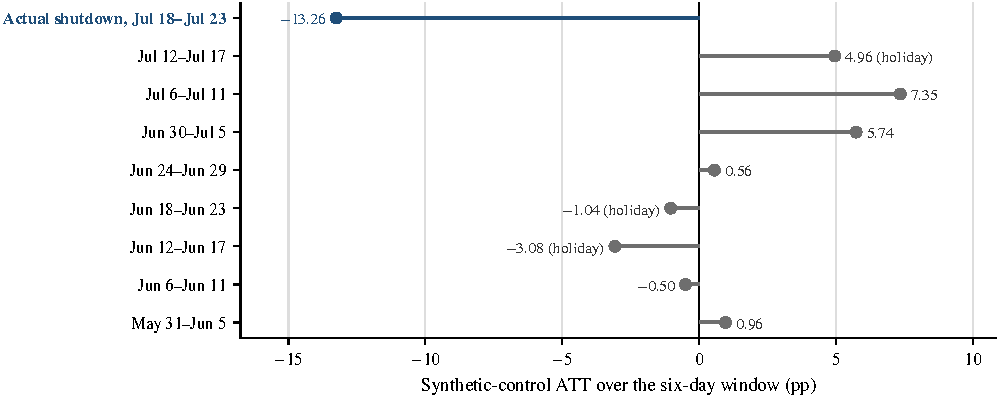
\includegraphics[width=\textwidth]{figA1_sc_intime_placebos.pdf}
\fignote{Each grey row is a six-day pre-treatment window chosen by the rule in \cref{sec:sc_diagnostics}; donor weights are re-estimated using only the days before each window, and the ATT is the mean gap between Bangladesh and its synthetic control over the window, as in the primary specification (blue row). ``Holiday'' marks windows containing a Bangladesh national holiday. All eight eligible windows are shown. Details in \cref{tab:sc_intime}. Source: \texttt{results/synthetic\_control/reproduced/sc\_intime\_placebos.csv}.}
\end{figure}

% Generated by analysis/tables/make_all_tables.py -- do not edit by hand.
\begin{table}[H]
\centering
\footnotesize
\caption{Synthetic-control in-time placebos}
\label{tab:sc_intime}
\begin{threeparttable}
\begin{tabular}{lrrrrrrl}
\toprule
Window (2024) & Fit days & ATT (pp) & Pre RMSPE & Ratio & Rank $|$ATT$|$ & Rank ratio & Holiday \\
\midrule
\textbf{Jul 18--Jul 23 (actual)} & 78 & $-$13.256 & 3.260 & 4.192 & 1 & 1 &  \\
Jul 12--Jul 17 & 72 & 4.958 & 3.032 & 1.787 & 4 & 5 & Ashura \\
Jul 6--Jul 11 & 66 & 7.349 & 2.279 & 3.376 & 2 & 3 &  \\
Jun 30--Jul 5 & 60 & 5.736 & 1.634 & 3.793 & 3 & 2 &  \\
Jun 24--Jun 29 & 54 & 0.560 & 1.685 & 0.654 & 8 & 9 &  \\
Jun 18--Jun 23 & 48 & $-$1.036 & 1.678 & 1.227 & 6 & 6 & Eid al-Adha \\
Jun 12--Jun 17 & 42 & $-$3.076 & 1.546 & 2.487 & 5 & 4 & Eid al-Adha \\
Jun 6--Jun 11 & 36 & $-$0.498 & 1.588 & 0.844 & 9 & 7 &  \\
May 31--Jun 5 & 30 & 0.964 & 1.683 & 0.720 & 7 & 8 &  \\
\bottomrule
\end{tabular}
\begin{tablenotes}[flushleft]
\footnotesize\raggedright
\item \textit{Notes:} Pre-specified rule: six-day pseudo-treatment windows, non-overlapping, moving backward from July 17, each with at least 28 days of fitting data from May 1. Donor weights are re-estimated for each window using only days before it; ATT and RMSPE definitions are those of the primary specification. Ranks are among the nine windows. The windows differ in fit length and are not exchangeable, so the ranks are descriptive and not a formal $p$-value. Source: \texttt{results/synthetic\_control/reproduced/sc\_intime\_placebos.csv}, computed by \texttt{analysis/synthetic\_control/03\_intime\_placebos.py}.
\end{tablenotes}
\end{threeparttable}
\end{table}


\subsection{International repository-domain diagnostics}
\label{app:sector_sc}

The following tables retain every country's coverage, all domain support decisions, and the fit and threshold diagnostics for the international extension. Missing estimates indicate insufficient support under the stated rule.

\begin{table}[H]
\centering
\small
\caption{International historical-text classification coverage}
\label{tab:sector_coverage}
\begin{threeparttable}
\begin{tabular}{@{}lrrrr@{}}
\toprule
Country & Eligible & README & Assigned & Assigned (\%) \\
\midrule
Bangladesh & 10,241 & 5,749 & 2,163 & 21.1 \\
Ghana & 1,373 & 892 & 318 & 23.2 \\
Indonesia & 10,965 & 6,810 & 2,678 & 24.4 \\
Jordan & 446 & 281 & 102 & 22.9 \\
Kenya & 3,553 & 2,264 & 870 & 24.5 \\
Malaysia & 1,396 & 916 & 343 & 24.6 \\
Morocco & 1,651 & 984 & 325 & 19.7 \\
Nepal & 2,373 & 1,272 & 444 & 18.7 \\
Nigeria & 6,961 & 4,442 & 1,552 & 22.3 \\
Pakistan & 7,276 & 4,209 & 1,512 & 20.8 \\
Philippines & 2,926 & 1,779 & 678 & 23.2 \\
Sri Lanka & 3,068 & 1,954 & 711 & 23.2 \\
Thailand & 2,317 & 1,526 & 581 & 25.1 \\
Tunisia & 1,012 & 577 & 230 & 22.7 \\
Vietnam & 3,600 & 2,182 & 898 & 24.9 \\
\bottomrule
\end{tabular}
\begin{tablenotes}[flushleft]
\footnotesize
\item Counts refer to users and their dominant pre-treatment repository. Assigned requires an available July 17 README and classifier score at least 0.80. Other eligible users remain unclassified; they are not removed from national estimates. Retrieval takes place in October 2026 and cannot recover every repository available in 2024.
\end{tablenotes}
\end{threeparttable}
\end{table}

\begin{table}[H]
\centering
\small
\caption{Pre-specified support screen for every domain}
\label{tab:sector_support}
\begin{threeparttable}
\begin{tabular}{@{}p{0.38\textwidth}rrr@{}}
\toprule
Domain & Bangladesh users & Eligible donors & Estimated \\
\midrule
Agriculture & 25 & 3 & No \\
Mining & 0 & 0 & No \\
Utilities & 8 & 0 & No \\
Construction & 1 & 0 & No \\
Manufacturing & 8 & 0 & No \\
Wholesale & 0 & 0 & No \\
Retail & 368 & 11 & Yes \\
Transport & 44 & 5 & Yes \\
Information & 518 & 14 & Yes \\
Finance & 90 & 9 & Yes \\
Real estate & 49 & 1 & No \\
Professional services & 151 & 11 & Yes \\
Administrative support & 36 & 1 & No \\
Education & 424 & 13 & Yes \\
Health & 155 & 5 & Yes \\
Arts and recreation & 72 & 7 & Yes \\
Accommodation and food & 192 & 4 & No \\
Other services & 18 & 1 & No \\
Public administration & 4 & 0 & No \\
Unclassified & 8078 & 14 & Yes \\
\bottomrule
\end{tabular}
\begin{tablenotes}[flushleft]
\footnotesize
\item At least 30 Bangladesh users and five donor countries with at least 30 users each are required. The rule uses sample support, not treatment-period effect size. Unreported estimates in the main table correspond to this screen, not a zero estimated effect.
\end{tablenotes}
\end{threeparttable}
\end{table}

\begin{table}[H]
\centering
\small
\caption{Sector-cohort fit and scale-adjusted placebo diagnostics}
\label{tab:sector_fit}
\begin{threeparttable}
\begin{tabular}{@{}p{0.27\textwidth}rrrr@{}}
\toprule
Domain & Pre RMSPE / mean & Holdout (pp) & Post/pre RMSPE & Ratio rank \\
\midrule
Retail & 0.15 & 3.57 & 5.43 & 0.083 \\
Transport & 0.51 & 5.16 & 1.96 & 0.167 \\
Information & 0.16 & 3.61 & 4.98 & 0.067 \\
Finance & 0.27 & 6.27 & 3.10 & 0.100 \\
Professional services & 0.24 & 5.24 & 4.18 & 0.083 \\
Education & 0.24 & 9.12 & 3.13 & 0.071 \\
Health & 0.32 & 6.20 & 2.40 & 0.167 \\
Arts and recreation & 0.31 & 6.65 & 2.32 & 0.125 \\
Unclassified & 0.20 & 7.50 & 3.89 & 0.067 \\
\bottomrule
\end{tabular}
\begin{tablenotes}[flushleft]
\footnotesize
\item The normalized fit divides pre-period RMSPE by mean pre-period activity. Holdout weights are fitted through June 30 and evaluated July 1--17, conditional on July 17 cohort definitions. Large errors limit counterfactual credibility. Ratio rank compares the shutdown/pre-period RMSPE ratio with sector-specific donor placebos.
\end{tablenotes}
\end{threeparttable}
\end{table}

\begin{table}[H]
\centering
\small
\caption{Sector-cohort ATT sensitivity to classification rules}
\label{tab:sector_sc_sensitivity}
\begin{threeparttable}
\begin{tabular}{@{}p{0.38\textwidth}rrrr@{}}
\toprule
Domain & 0.70 & 0.80 & 0.90 & Name fallback \\
\midrule
Accommodation and food & -14.56 & -- & -- & -15.71 \\
Arts and recreation & -11.61 & -12.33 & -- & -10.90 \\
Education & -16.30 & -15.04 & -15.83 & -14.15 \\
Finance & -10.97 & -12.28 & -12.10 & -12.59 \\
Health & -16.10 & -16.84 & -16.65 & -15.89 \\
Information & -13.07 & -12.74 & -12.50 & -12.70 \\
Professional services & -14.34 & -16.13 & -- & -16.13 \\
Retail & -16.47 & -15.69 & -15.16 & -14.31 \\
Transport & -10.95 & -11.31 & -- & -11.90 \\
Unclassified & -12.76 & -12.77 & -12.92 & -12.58 \\
\bottomrule
\end{tabular}
\begin{tablenotes}[flushleft]
\footnotesize
\item Effects in percentage points. The first three columns require a historical README. The final column admits classifications from names alone at score 0.80. Each rule changes the fixed cohort and may change donor support. A dash means insufficient support, not a zero effect; columns are therefore not estimates for an identical population.
\end{tablenotes}
\end{threeparttable}
\end{table}


\begin{figure}[H]
\centering
\caption{Observed and synthetic paths for all supported repository-domain cohorts}
\label{fig:advisor_sector_paths}
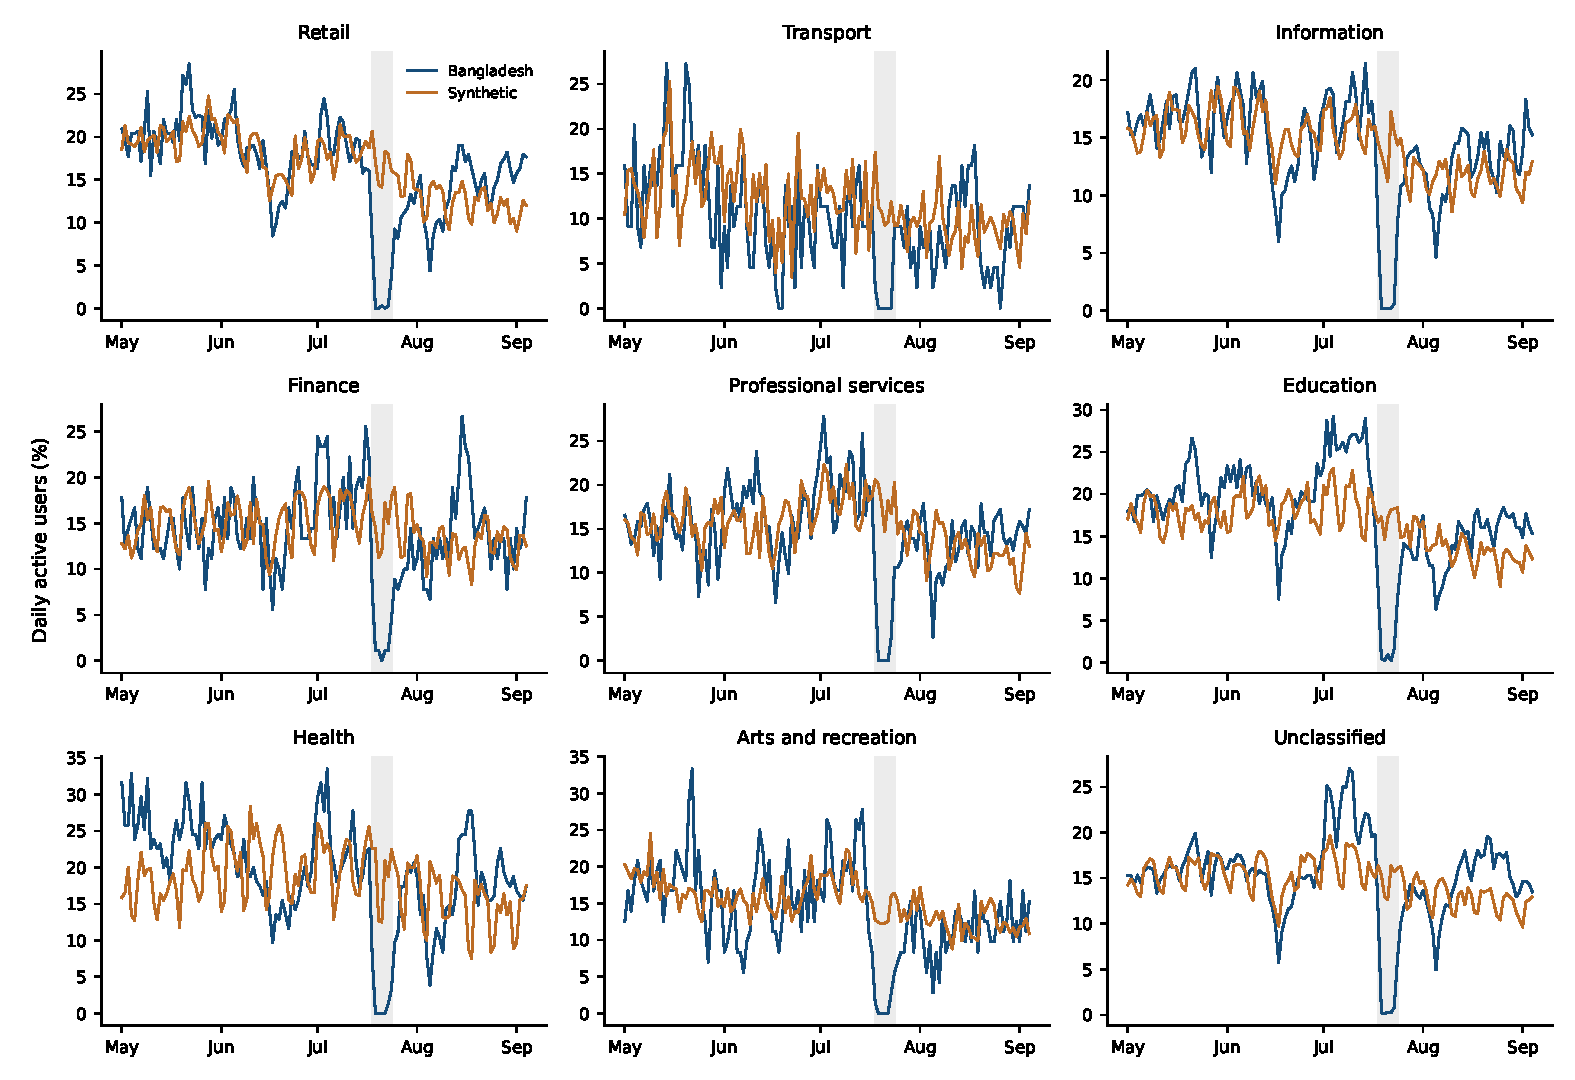
\includegraphics[width=\textwidth,height=0.76\textheight,keepaspectratio]{fig_advisor_sector_paths.pdf}
\fignote{Fixed pre-treatment user cohorts; historical README and score at least 0.80. Grey marks July 18--23, the primary estimand. Paths after July 23 are descriptive and use the same pre-fitted weights. Panel scales vary. Full domain-country weights, donor placebos and leave-one-out estimates are retained in the replication outputs.}
\end{figure}

\subsection{Difference-in-differences and event study}

% Generated by analysis/tables/make_all_tables.py -- do not edit by hand.
\begin{table}[H]
\centering
\footnotesize
\caption{Aggregate event study: all weekly estimates}
\label{tab:did_es_full}
\begin{threeparttable}
\begin{tabular}{lllrrrr}
\toprule
Week & Dates (2024) & Days & $\hat\theta_k$ (pp) & Placebo-based interval & Placebo range & Rank $p$ \\
\midrule
$-11$ & May 1--May 8 & 8 & $-$0.86 & [$-$4.37, 2.65] & [$-$1.68, 4.62] & 0.6000 \\
$-10$ & May 9--May 15 & 7 & $-$1.83 & [$-$4.50, 0.84] & [$-$2.23, 2.49] & 0.2667 \\
$-9$ & May 16--May 22 & 7 & 0.58 & [$-$1.21, 2.36] & [$-$1.06, 2.46] & 0.4667 \\
$-8$ & May 23--May 29 & 7 & $-$0.51 & [$-$2.47, 1.45] & [$-$2.36, 1.92] & 0.4667 \\
$-7$ & May 30--Jun 5 & 7 & $-$0.05 & [$-$2.08, 1.97] & [$-$1.72, 2.02] & 1.0000 \\
$-6$ & Jun 6--Jun 12 & 7 & $-$1.23 & [$-$3.28, 0.81] & [$-$0.99, 2.54] & 0.2000 \\
$-5$ & Jun 13--Jun 19 & 7 & $-$4.89 & [$-$9.31, $-$0.47] & [$-$3.64, 2.34] & 0.0667 \\
$-4$ & Jun 20--Jun 26 & 7 & $-$2.71 & [$-$5.13, $-$0.29] & [$-$3.06, 1.62] & 0.1333 \\
$-3$ & Jun 27--Jul 3 & 7 & 1.67 & [$-$0.46, 3.80] & [$-$1.31, 1.45] & 0.0667 \\
$-2$ & Jul 4--Jul 10 & 7 & 6.10 & [3.76, 8.43] & [$-$1.74, 1.62] & 0.0667 \\
$-1$ & Jul 11--Jul 17 & 7 & 3.86 & [2.15, 5.58] & [$-$1.63, 0.98] & 0.0667 \\
$0$ & Jul 18--Jul 23 & 6 & $-$13.09 & [$-$15.39, $-$10.79] & [$-$1.72, 1.60] & 0.0667 \\
$+1$ & Jul 24--Jul 30 & 7 & $-$2.66 & [$-$5.35, 0.02] & [$-$1.95, 2.23] & 0.0667 \\
$+2$ & Jul 31--Aug 6 & 7 & $-$2.76 & [$-$4.87, $-$0.65] & [$-$1.22, 2.56] & 0.0667 \\
$+3$ & Aug 7--Aug 13 & 7 & 0.52 & [$-$1.99, 3.02] & [$-$1.87, 2.73] & 0.9333 \\
$+4$ & Aug 14--Aug 20 & 7 & 4.31 & [1.99, 6.64] & [$-$1.82, 2.77] & 0.0667 \\
$+5$ & Aug 21--Aug 27 & 7 & 4.84 & [2.40, 7.28] & [$-$1.48, 2.71] & 0.0667 \\
$+6$ & Aug 28--Sep 3 & 7 & 2.53 & [0.01, 5.05] & [$-$2.32, 2.31] & 0.0667 \\
\bottomrule
\end{tabular}
\begin{tablenotes}[flushleft]
\footnotesize\raggedright
\item \textit{Notes:} $\hat\theta_k$ from \cref{eq:es_agg}, relative to the May 1--July 17 mean. Week $-11$ includes May 1; September 4 (a partial week) is omitted. \textit{Placebo range}: minimum and maximum of the 14 in-space placebo estimates. \textit{Placebo-based interval}: $\hat\theta_k\pm1.96$ times the placebo standard deviation; a donor-placebo reference interval, not a conventional confidence interval. Other definitions as in \cref{tab:did}. Source: \texttt{results/did/did\_eventstudy\_weekly.csv}.
\end{tablenotes}
\end{threeparttable}
\end{table}

% Generated by analysis/tables/make_all_tables.py -- do not edit by hand.
\begin{table}[H]
\centering
\footnotesize
\caption{International difference-in-differences by outcome}
\label{tab:did_secondary}
\begin{threeparttable}
\begin{tabular}{lrrrr}
\toprule
& \multicolumn{2}{c}{All days} & \multicolumn{2}{c}{Holidays excluded} \\
\cmidrule(lr){2-3}\cmidrule(lr){4-5}
Outcome & ATT & Relative & ATT & Relative \\
\midrule
Active-user rate (primary) & $-$13.088 & $-$86.6\% & $-$13.379 & $-$86.9\% \\
Productive active rate & $-$14.669 & $-$86.1\% & $-$14.975 & $-$86.3\% \\
Shipping active rate & $-$0.771 & $-$90.4\% & $-$0.806 & $-$90.8\% \\
Collaboration active rate & $-$0.302 & $-$84.9\% & $-$0.311 & $-$85.3\% \\
Collaboration events / 1,000 & $-$10.855 & $-$89.7\% & $-$11.532 & $-$90.2\% \\
Shipping output / 1,000 & $-$14.017 & $-$90.0\% & $-$14.631 & $-$90.4\% \\
\bottomrule
\end{tabular}
\begin{tablenotes}[flushleft]
\footnotesize\raggedright
\item \textit{Notes:} Aggregate DiD as in \cref{tab:did}, Panel A, for each outcome; rates in percentage points, counts per 1,000 eligible users. No placebo inference is stored for these specifications. Source: \texttt{results/final/table\_DiD\_all\_outcomes.csv}.
\end{tablenotes}
\end{threeparttable}
\end{table}



\subsection{Regression discontinuity in time}
\label{app:rdit_detail}
\label{sec:rdit_method}

A regression discontinuity in time provides a third temporal comparison. The archived preferred specification uses a cutoff at July 17, 2024, a bandwidth of $h=7$ days (July 10--24, fifteen daily observations), and a local linear fit on each side. With $\tilde{t} = t - \text{July 17}$ and $D_t = \mathbf{1}\{\tilde{t} \geq 0\}$, so that July 17 itself lies on the post-cutoff side, I estimate
\begin{equation}
  Y_{t} = \alpha + \tau D_{t} + \gamma_{1}\tilde{t} + \gamma_{2} D_{t}\tilde{t} + u_{t},
  \qquad |\tilde{t}| \leq h,
  \label{eq:rdit}
\end{equation}
where $\tau$ is the discontinuity and $Y_t$ is the daily share of users with at least one productive GitHub event in a balanced user-day panel of 10,329 Bangladesh-associated and 3,025 Philippines-associated accounts. This eligible sample differs slightly from the 10,241 Bangladesh accounts of the country-day panel used for the synthetic control. I estimate \cref{eq:rdit} for Bangladesh, for the Bangladesh-minus-Philippines gap as a controlled specification, and for the Philippines alone as a geographic placebo. Inference uses heteroskedasticity-and-autocorrelation-consistent (HAC) Newey--West standard errors with two lags, following the cautions in \citet{hausman2018} regarding serial correlation in time-series discontinuity designs. Because time itself is the running variable and other contemporaneous events can occur at the same date, the RDiT is interpreted as a robustness check rather than a standalone source of causal identification.

The July 17 cutoff reproduces the original preferred specification; it is not chosen because it yields a preferred estimate. No daily cutoff matches the event exactly: provider-level mobile outages began late on July 17 UTC, whereas the nationwide near-total cutoff occurred around 15:00 UTC on July 18 \citep{belson2024}. I therefore report a complete grid of July 17, 18, and 19 cutoffs crossed with 4-, 5-, 7-, 10-, and 14-day bandwidths in \cref{tab:rdit_grid}, together with the separate archived 16-specification grid in \cref{tab:rdit_arch_grid}. An hourly design would require a separate specification and is not pursued here.


\subsubsection{Results}
\label{sec:rdit_results}

\Cref{fig:rdit} shows the daily series used in the RDiT. In Bangladesh, the share of users with productive activity is 19.03 percent on July 17, falls to 10.74 percent on July 18, and lies between 0.48 and 1.23 percent from July 19 through July 23 before recovering gradually from July 24. The Philippines, used as a geographic placebo, shows no comparable break.

\begin{figure}[htbp]
\centering
\caption{Regression discontinuity in time: daily share of users with productive activity around the July 17 cutoff (visual companion to \cref{tab:rdit})}
\label{fig:rdit}
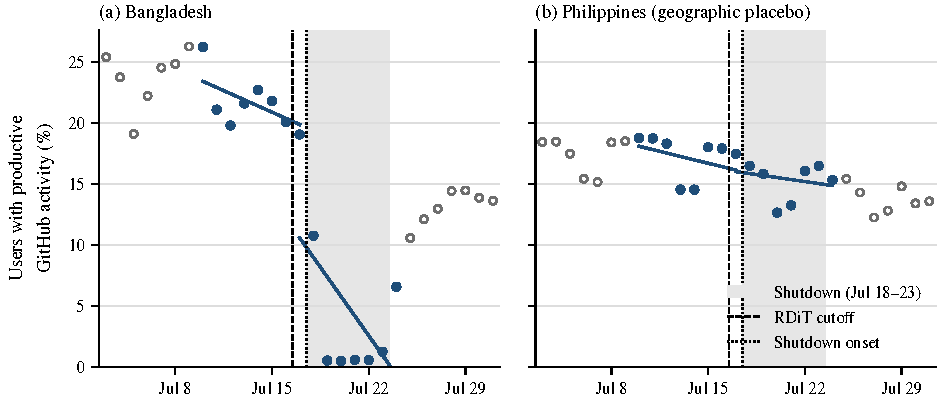
\includegraphics[width=\textwidth]{fig7_rdit_cutoff.pdf}
\fignote{Daily percentage of users with productive GitHub activity in the balanced user-day panels used for the RDiT (10,329 Bangladesh-associated and 3,025 Philippines-associated accounts). Filled markers are the fifteen days in the 7-day bandwidth of \cref{eq:rdit}. Lines are the fits of the archived preferred specification and correspond exactly to \cref{tab:rdit}. Dashed line: cutoff, with July 17 on the post-cutoff side; dotted line: shutdown boundary between July 17 and 18; shaded: July 18--23 shutdown. The RDiT is a temporal robustness check, not the primary design. Source: Author's calculations using GH Archive.}
\end{figure}

The RDiT produces a smaller point estimate but the same qualitative conclusion (\cref{tab:rdit}). The archived preferred local linear specification estimates a discontinuity of $-$9.28 percentage points in Bangladesh's active-user rate; a controlled Bangladesh-minus-Philippines version yields $-$9.16 percentage points. HAC $p$-values are approximately 0.065 in both cases, while the Philippines placebo is near zero. The smaller magnitude than in the synthetic control and DiD is consistent with the design visible in \cref{fig:rdit}: the cutoff day, July 17, precedes the shutdown but lies on the post-cutoff side, and the linear post-cutoff fit spans both the collapse and the beginning of the recovery on July 24.
Because \citet{hausman2018} urge caution in interpreting RDiT estimates, I emphasize the direction and timing of the break rather than treating the RDiT $p$-value as the decisive inferential statistic.

% Generated by analysis/tables/make_all_tables.py -- do not edit by hand.
\begin{table}[H]
\centering
\footnotesize
\caption{Regression discontinuity in time: preferred specification}
\label{tab:rdit}
\begin{threeparttable}
\begin{tabular}{l>{\raggedright\arraybackslash}p{3.3cm}rrcrr}
\toprule
Specification & Outcome & Effect (pp) & HAC SE & 95\% CI & $p$ & Days \\
\midrule
Main local linear & Bangladesh active rate & $-$9.284 & 5.034 & [$-$19.151, 0.584] & 0.065 & 15 \\
Controlled local linear & Bangladesh $-$ Philippines active rate & $-$9.160 & 4.980 & [$-$18.921, 0.601] & 0.066 & 15 \\
Geographic placebo & Philippines active rate & $-$0.124 & 1.492 & [$-$3.048, 2.801] & 0.934 & 15 \\
\bottomrule
\end{tabular}
\begin{tablenotes}[flushleft]
\footnotesize\raggedright
\item \textit{Notes:} Local linear RDiT at the July 17, 2024 cutoff, bandwidth 7 days, polynomial degree 1, no donut, HAC lags 2. Effects are reported in percentage points. RDiT is a temporal robustness check, not the primary causal design. Source: \texttt{results/rdit/main\_rdit\_summary.csv}.
\end{tablenotes}
\end{threeparttable}
\end{table}


The RDiT grid spans $-$4.45 to $-$19.52 percentage points for Bangladesh, illustrating substantial specification sensitivity (\cref{tab:rdit_grid}). The archived 16-row grid is also retained, but its input and cutoff provenance is unresolved. The RDiT sample includes 174 accounts absent from the main synthetic-control cohort, while 86 accounts in that cohort are absent from the RDiT sample; the difference is not simply 88 additional accounts. These facts limit a direct comparison of the two levels and estimates.


% Generated by analysis/tables/make_all_tables.py -- do not edit by hand.
\begin{table}[H]
\centering
\small
\caption{RDiT: complete cutoff and bandwidth grid}
\label{tab:rdit_grid}
\begin{threeparttable}
\begin{tabular*}{\textwidth}{@{\extracolsep{\fill}}llrrr}
\toprule
Cutoff & $h$ & Bangladesh & BD minus PH & Philippines \\
\midrule
07-17 & 4 & -4.45 (3.45) & -2.40 (3.43) & -2.05 (0.53) \\
07-17 & 5 & -7.30 (4.36) & -6.56 (4.87) & -0.74 (1.54) \\
07-17 & 7 & -9.28 (5.03) & -9.16 (4.98) & -0.12 (1.49) \\
07-17 & 10 & -13.70 (6.05) & -13.07 (5.80) & -0.62 (1.35) \\
07-17 & 14 & -16.80 (5.64) & -16.04 (5.35) & -0.76 (1.16) \\
07-18 & 4 & -11.09 (2.72) & -7.47 (2.14) & -3.62 (2.01) \\
07-18 & 5 & -12.98 (3.12) & -8.75 (1.94) & -4.24 (1.86) \\
07-18 & 7 & -17.49 (4.48) & -15.58 (4.29) & -1.91 (1.34) \\
07-18 & 10 & -18.06 (3.94) & -17.35 (4.18) & -0.71 (1.31) \\
07-18 & 14 & -19.52 (3.47) & -17.82 (3.50) & -1.70 (1.07) \\
07-19 & 4 & -9.00 (2.49) & -6.69 (2.12) & -2.31 (1.44) \\
07-19 & 5 & -11.54 (2.91) & -7.73 (1.99) & -3.81 (1.84) \\
07-19 & 7 & -16.59 (4.24) & -13.80 (4.06) & -2.79 (1.19) \\
07-19 & 10 & -16.76 (3.15) & -15.52 (3.59) & -1.23 (1.17) \\
07-19 & 14 & -17.60 (2.99) & -15.50 (3.16) & -2.10 (1.00) \\
\bottomrule
\end{tabular*}
\begin{tablenotes}[flushleft]
\footnotesize\raggedright
\item \textit{Notes:} All effects and HAC(2) standard errors in percentage points. Local linear fits with separate slopes, cutoff day on the right, inclusive symmetric bandwidth, $n/(n-4)$ variance correction. All 45 fits are reported; none replaces the archived July 17, $h=7$ result. Source: new round-2 diagnostic grid.
\end{tablenotes}
\end{threeparttable}
\end{table}

% Generated by analysis/tables/make_all_tables.py -- do not edit by hand.
\begin{table}[H]
\centering
\small
\caption{RDiT: preserved archived 16-specification grid}
\label{tab:rdit_arch_grid}
\begin{threeparttable}
\begin{tabular*}{\textwidth}{@{\extracolsep{\fill}}rlrrrr}
\toprule
Pre bandwidth & Polynomial & Donut & Effect (pp) & SE (pp) & $n$ \\
\midrule
7 & lin & False & -14.0 & 2.2 & 14 \\
7 & lin & True & -20.4 & 1.5 & 12 \\
7 & quad pre & False & -16.1 & 2.8 & 14 \\
7 & quad pre & True & -21.2 & 2.5 & 12 \\
10 & lin & False & -13.1 & 1.9 & 17 \\
10 & lin & True & -18.5 & 1.0 & 15 \\
10 & quad pre & False & -15.2 & 2.7 & 17 \\
10 & quad pre & True & -20.5 & 1.7 & 15 \\
14 & lin & False & -14.8 & 2.4 & 21 \\
14 & lin & True & -20.6 & 1.5 & 19 \\
14 & quad pre & False & -13.2 & 2.3 & 21 \\
14 & quad pre & True & -18.1 & 1.4 & 19 \\
21 & lin & False & -17.7 & 3.2 & 28 \\
21 & lin & True & -23.7 & 2.5 & 26 \\
21 & quad pre & False & -12.4 & 2.1 & 28 \\
21 & quad pre & True & -17.5 & 1.2 & 26 \\
\bottomrule
\end{tabular*}
\begin{tablenotes}[flushleft]
\footnotesize\raggedright
\item \textit{Notes:} Transcribed without re-estimation from data/processed/table3\_rdit\_sensitivity.csv. The historical cutoff, outcome, sample and variance procedure are not documented. The row labelled linear, 7 days, no donut is -14.0 pp, compared with -9.28 pp in the reproduced preferred specification; this is an unresolved provenance conflict, not evidence that one specification should replace the other.
\end{tablenotes}
\end{threeparttable}
\end{table}


\subsection{Mechanism}

\begin{table}[H]
\centering
\small
\caption{Repository-domain composition of residual-activity cohorts}
\label{tab:residual_domains}
\begin{threeparttable}
\begin{tabular}{@{}p{0.34\textwidth}rrrr@{}}
\toprule
Pre-treatment domain & \shortstack{All\\eligible} & \shortstack{Core\\publishers} & \shortstack{Onset\\authors} & \shortstack{Delayed\\authors} \\
\midrule
Accommodation and food & 192 & 0 & 4 & 3 \\
Administrative support & 36 & 0 & 0 & 0 \\
Agriculture & 25 & 0 & 1 & 1 \\
Arts and recreation & 72 & 0 & 4 & 2 \\
Construction & 1 & 0 & 0 & 0 \\
Education & 424 & 4 & 18 & 13 \\
Finance & 90 & 1 & 1 & 1 \\
Health & 155 & 0 & 5 & 3 \\
Information & 518 & 1 & 11 & 10 \\
Manufacturing & 8 & 0 & 0 & 0 \\
Other services & 18 & 0 & 0 & 0 \\
Professional services & 151 & 0 & 5 & 2 \\
Public administration & 4 & 0 & 0 & 0 \\
Real estate & 49 & 0 & 1 & 1 \\
Retail & 368 & 1 & 6 & 5 \\
Transport & 44 & 0 & 0 & 0 \\
Unclassified & 8,078 & 32 & 192 & 149 \\
Utilities & 8 & 1 & 2 & 1 \\
\bottomrule
\end{tabular}
\begin{tablenotes}[flushleft]
\footnotesize
\item Counts, not effects. Historical README classification at score 0.80; all unclassified accounts remain visible. Cohorts overlap and have the definitions in the mechanism section. Small cells and substantial unclassified coverage do not establish occupational specialization.
\end{tablenotes}
\end{threeparttable}
\end{table}


% Generated by analysis/tables/make_all_tables.py -- do not edit by hand.
\begin{table}[H]
\centering
\small
\caption{Mechanism placebo comparison}
\label{tab:mech_placebos}
\begin{threeparttable}
\begin{tabular}{lrrr}
\toprule
Metric & Real shutdown & Mean placebo & Maximum placebo \\
\midrule
Released in next 6 days & 25.38\% & 0.56\% & 0.77\% \\
Delay $>$24h & 29.71\% & 1.10\% & 1.31\% \\
Delay $>$48h & 25.38\% & 0.72\% & 0.90\% \\
Delay $>$72h & 22.75\% & 0.46\% & 0.56\% \\
Delay $>$120h & 13.88\% & 0.32\% & 0.46\% \\
\bottomrule
\end{tabular}
\begin{tablenotes}[flushleft]
\footnotesize\raggedright
\item \textit{Notes:} Placebo windows are six six-day authoring windows between July 1 and July 11, with six-day subsequent release windows that end before treatment. Windows overlap, so the comparison is descriptive rather than an exact independent randomization test.
\end{tablenotes}
\end{threeparttable}
\end{table}

% Generated by analysis/tables/make_all_tables.py -- do not edit by hand.
\begin{table}[H]
\centering
\footnotesize
\caption{Metadata coverage by push period}
\label{tab:metadata}
\begin{threeparttable}
\begin{tabular}{lrrrrr}
\toprule
Period & Target $N$ & Commit found & Author timestamp & Author login & Author = pusher \\
\midrule
Pre & 17,000 & 82.34\% & 82.34\% & 77.95\% & 71.49\% \\
Shutdown & 3,197 & 84.24\% & 84.24\% & 79.17\% & 69.69\% \\
Post & 65,868 & 81.81\% & 81.81\% & 77.81\% & 71.05\% \\
\bottomrule
\end{tabular}
\begin{tablenotes}[flushleft]
\footnotesize\raggedright
\item \textit{Notes:} Similar resolution rates across periods reduce concern that the mechanism result is generated by treatment-specific metadata missingness.
\end{tablenotes}
\end{threeparttable}
\end{table}

% Generated by analysis/tables/make_all_tables.py -- do not edit by hand.
\begin{table}[H]
\centering
\footnotesize
\caption{Push-listing completeness by period}
\label{tab:push_completeness}
\begin{threeparttable}
\begin{tabular}{lrrrrr}
\toprule
Period & Pushes & Mean push size & Complete pushes & Nominal commits & Commits in complete pushes \\
\midrule
Pre & 121,960 & 1.29 & 99.78\% & 157,834 & 90.27\% \\
Shutdown & 2,738 & 1.70 & 99.53\% & 4,667 & 73.11\% \\
Post & 58,110 & 1.69 & 99.66\% & 98,022 & 71.45\% \\
\bottomrule
\end{tabular}
\begin{tablenotes}[flushleft]
\footnotesize\raggedright
\item \textit{Notes:} A push is complete when its historical payload lists every commit. Large pushes account for a disproportionate share of commits and are more likely to be incomplete. Source: \texttt{results/mechanism/robust\_push\_size\_period.csv}.
\end{tablenotes}
\end{threeparttable}
\end{table}

% Generated by analysis/tables/make_all_tables.py -- do not edit by hand.
\begin{table}[H]
\centering
\footnotesize
\caption{Mechanism estimates by push size}
\label{tab:push_size}
\begin{threeparttable}
\begin{tabular}{lrrrrrr}
\toprule
Sample & $N$ & Backlog $N$ & Backlog share & $>$24h & $>$48h & $>$72h \\
\midrule
All complete pushes & 2,932 & 829 & 28.27\% & 29.71\% & 25.38\% & 22.75\% \\
Push size $\leq$ 10 & 2,503 & 526 & 21.01\% & 21.81\% & 18.98\% & 17.14\% \\
Push size $\leq$ 5 & 2,217 & 320 & 14.43\% & 15.07\% & 13.62\% & 12.45\% \\
Push size $\leq$ 2 & 1,947 & 151 & 7.76\% & 7.96\% & 7.29\% & 6.93\% \\
Single-commit pushes & 1,707 & 57 & 3.34\% & 3.28\% & 2.93\% & 2.75\% \\
\bottomrule
\end{tabular}
\begin{tablenotes}[flushleft]
\footnotesize\raggedright
\item \textit{Notes:} Strict \texttt{authoredDate} sample of commits authored July 18--23. The backlog share is not invariant to push size.
\end{tablenotes}
\end{threeparttable}
\end{table}

% Generated by analysis/tables/make_all_tables.py -- do not edit by hand.
\begin{table}[H]
\centering
\small
\caption{Concentration of the backlog across users and repositories}
\label{tab:concentration}
\begin{threeparttable}
\begin{tabular}{lr}
\toprule
Statistic & Value \\
\midrule
Shutdown-authored commits & 2,932 \\
Backlog commits & 829 (28.27\%) \\
Users / with backlog & 835 / 222 (26.59\%) \\
Repositories / with backlog & 977 / 246 (25.18\%) \\
Largest user's share of backlog & 2.77\% \\
Top 5 users' share of backlog & 12.06\% \\
Top 10 users' share of backlog & 21.47\% \\
\midrule \multicolumn{2}{l}{\textit{Backlog share after dropping top-$k$ backlog users}} \\
$k=1$ ($N=2,909$) & 27.71\% \\
$k=3$ ($N=2,868$) & 26.67\% \\
$k=5$ ($N=2,831$) & 25.75\% \\
$k=10$ ($N=2,739$) & 23.77\% \\
$k=20$ ($N=2,577$) & 20.37\% \\
\bottomrule
\end{tabular}
\begin{tablenotes}[flushleft]
\footnotesize\raggedright
\item \textit{Notes:} Strict \texttt{authoredDate} sample. Users are ranked by their number of backlog commits.
\end{tablenotes}
\end{threeparttable}
\end{table}


\subsection{Within-Bangladesh sectoral recovery}
\label{sec:sector_method}

The designs above estimate the effect of the shutdown during July 18--23. To describe how activity evolved after restoration, I use the fixed sample of 20,000 accounts described in \cref{sec:sector_data}. For user $i$, sector $s$, and day $t$, let $A_{ist}=1$ if the user records at least one PushEvent on day $t$ in a repository classified to sector $s$; activity in several repositories of the same sector on the same day counts once. Days are grouped into event periods $k$: the final eight complete pre-shutdown weeks, $k=-8,\dots,-1$ (May 23--July 17, 2024); the shutdown, $k=0$ (July 18--23); and consecutive seven-day bins after it, starting with $k=+1$ (July 24--30). Let $\bar{A}_{isk}$ be user $i$'s share of active days in period $k$, and $\bar{A}^{\mathrm{pre}}_{is}$ the corresponding share over the 56 baseline days. I report
\begin{equation}
  \beta_{sk} = \frac{100}{N}\sum_{i=1}^{N}\bigl(\bar{A}_{isk} - \bar{A}^{\mathrm{pre}}_{is}\bigr),
  \qquad
  R_{sk} = 100 \times \frac{\sum_{i} \bar{A}_{isk}}{\sum_{i} \bar{A}^{\mathrm{pre}}_{is}},
  \label{eq:sector}
\end{equation}
where $N=20{,}000$ and users without activity in sector $s$ contribute zeros. The coefficient $\beta_{sk}$ is the change in the daily probability of sector-$s$ push activity relative to the baseline, in percentage points; the recovery index $R_{sk}$ normalizes the baseline to 100. Standard errors for $\beta_{sk}$ are 100 times the standard deviation of the user-level differences divided by $\sqrt{N}$, and 95 percent intervals use the normal approximation. As a summary of recovery timing, I report the first post-shutdown week that begins two consecutive weeks with $R_{sk}\geq 80$.

Because the activity measure counts pushes to any classified repository, including repositories first observed after the shutdown, it captures recovery through new projects and through switching across repositories. As a complementary specification, I also follow only the repositories pushed to during the baseline weeks, whose activity cannot be replaced by new projects.

This analysis compares each sector with its own pre-shutdown baseline and has no untreated comparison group. It therefore describes the heterogeneity and timing of recovery within Bangladesh; it does not estimate sector-specific causal effects. Post-shutdown deviations from the baseline may also reflect trends, seasonality, or other Bangladesh-specific developments. The confidence intervals capture sampling variation across users but not common shocks that affect all users in a given week. The pre-shutdown coefficients ($k<0$) indicate how much weekly activity fluctuates around the baseline in the absence of a shutdown and serve as a benchmark for interpreting post-shutdown deviations.

\subsection{Sectoral recovery after restoration}
\label{sec:sector_results}

The synthetic-control estimates describe the collapse during the shutdown window. They do not show how activity evolved once connectivity returned, or whether recovery was common across the kinds of projects on which Bangladeshi developers work. This subsection addresses both questions using the fixed sample of 20,000 Bangladesh-associated accounts and the repository-sector classification of \cref{sec:sector_data}, estimated as described in \cref{sec:sector_method}. The analysis compares each sector with its own pre-shutdown baseline. It documents heterogeneity in recovery dynamics within Bangladesh; it does not estimate sector-specific causal effects relative to an untreated international control, and the synthetic-control estimate in \cref{sec:main_results} remains the paper's headline result. Throughout, a sector refers to the economic sector associated with the repositories in which observable GitHub activity occurs, not to developers' employers or industries of employment.

% Generated by analysis/tables/make_all_tables.py -- do not edit by hand.
\begin{table}[htbp]
\centering
\footnotesize
\caption{Recovery of observable GitHub push activity by repository sector}
\label{tab:sector_recovery}
\begin{threeparttable}
\begin{tabular}{lrrrrrrrrr}
\toprule
& & Pre & Pre rate & \multicolumn{5}{c}{Recovery index (pre-period mean = 100)} & First wk \\
\cmidrule(lr){5-9}
Sector & NAICS & users & (\%) & Shutdown & +1 & +2 & +4 & +8 & $\geq$80, 2 wks \\
\midrule
Finance & 52 & 382 & 0.078 & 30.9 & 92.2 & 67.6 & 89.5 & 91.3 & 3 \\
Information & 51 & 1,528 & 0.442 & 11.7 & 75.9 & 72.2 & 106.0 & 94.5 & 3 \\
Education & 61 & 1,234 & 0.385 & 11.7 & 59.1 & 53.4 & 75.4 & 81.9 & 6 \\
Health & 62 & 514 & 0.132 & 6.3 & 40.7 & 51.5 & 77.5 & 89.4 & 6 \\
Retail & 44--45 & 1,012 & 0.295 & 6.2 & 52.0 & 52.3 & 153.7 & 79.6 & 9 \\
Real Estate & 53 & 213 & 0.063 & 4.0 & 33.0 & 25.1 & 44.4 & 85.5 & 5 \\
Accommodation/Food & 72 & 480 & 0.144 & 3.5 & 44.3 & 42.8 & 54.2 & 62.6 & -- \\
\bottomrule
\end{tabular}
\begin{tablenotes}[flushleft]
\footnotesize\raggedright
\item \textit{Notes:} Fixed sample of 20,000 Bangladesh-associated accounts. Repository sectors from the historical-README classifier with confidence $\geq$ 0.80. The outcome is the share of sampled users with at least one PushEvent to a repository of the sector on a given day. \textit{Pre users}: sampled users with such activity in the baseline period. \textit{Pre rate}: mean daily outcome over the baseline period (May 23--July 17, 2024, the final eight complete pre-shutdown weeks), in percent of all 20,000 users. Shutdown: July 18--23; week +1: July 24--30; subsequent 7-day bins. \textit{First wk $\geq$80, 2 wks}: first post-shutdown week that begins two consecutive weeks with an index of at least 80 (observed through week +17, November 13--19); it does not imply that the index stays above 80 thereafter. -- indicates no such week. Within-Bangladesh comparison with the sector's own pre-period; not a causal effect relative to an untreated control. Sources: \texttt{results/sector\_recovery/sectorwide/sectorwide\_recovery\_summary.csv}, verified against \texttt{results/sector\_recovery/final/table\_sector\_recovery\_main.csv}.
\end{tablenotes}
\end{threeparttable}
\end{table}


All seven sectors show a sharp fall in observable push activity during July 18--23 (\cref{tab:sector_recovery,fig:sector_index}). The shutdown-period recovery index ranges from 3.5 in Accommodation/Food to 11.7 in Information and Education and 30.9 in Finance. In every sector, the 95 percent confidence interval for the change relative to the baseline excludes zero (Appendix \cref{fig:sector_es}).

Restoration of connectivity did not imply an immediate or uniform recovery. In the first week after the shutdown (July 24--30), the recovery index ranges from 33.0 in Real Estate to 92.2 in Finance. Mobile connectivity returned only during this week, later than fixed broadband \citep{belson2024}, so part of the week $+1$ shortfall may reflect incomplete restoration. Recovery was also not monotonic: in Finance, Information, Education, Real Estate, and Accommodation/Food, the index is lower in week $+2$ (July 31--August 6) than in week $+1$. This week includes the renewed mobile shutdown on August 4 and the nationwide disruption on August 5 \citep{belson2024q3}, alongside unrest and initially declared holidays. These overlapping events prevent a separate attribution of the second-week decline. The stored holiday labels extend through August 7, although offices were ordered to reopen on August 6 \citep{bss2024reopen}; I keep the stored labels and document the discrepancy in the replication materials.

\begin{figure}[htbp]
\centering
\caption{Recovery of observable GitHub push activity by repository sector}
\label{fig:sector_index}
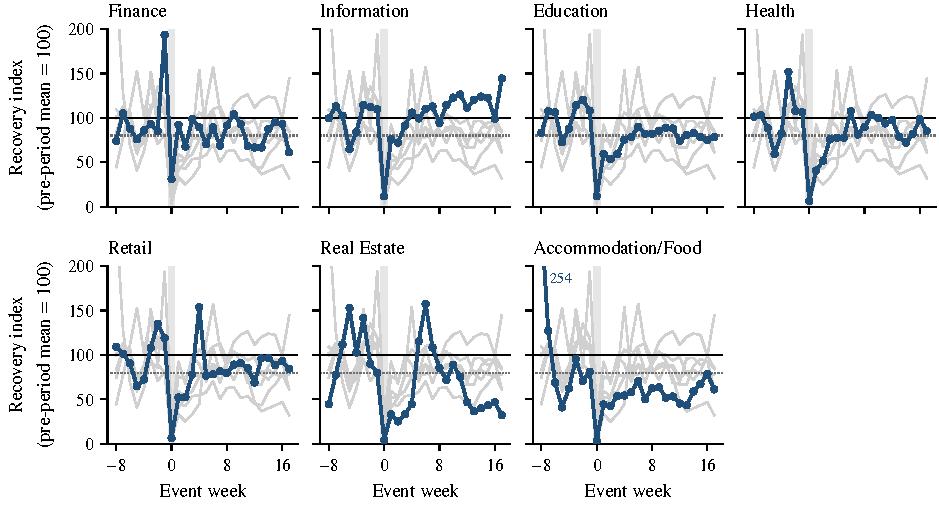
\includegraphics[width=\textwidth]{fig5_sector_recovery_index.pdf}
\fignote{Each panel highlights one sector's recovery index $R_{sk}$ (\cref{eq:sector}), 100 times its mean daily probability of push activity in event week $k$ relative to May 23--July 17, 2024; other sectors in grey. Shaded: July 18--23 shutdown; week $+1$ is July 24--30, and the window ends at week $+17$ (November 13--19). Lines mark 100 and 80; the one value above 200 is labeled. Fixed sample of 20,000 Bangladesh-associated accounts; sectors from a README classifier with confidence $\geq 0.80$ \citep{quispe2026naics} describe the repositories in which activity occurs, not developers' employers. Within-Bangladesh descriptive comparison, not a causal effect. Source: Author's calculations using GH Archive.}
\end{figure}

Finance and Information recovered fastest. Finance returned to an index of 92.2 in week $+1$, and both sectors begin a run of two consecutive weeks at or above 80 in week $+3$. Information exceeds its baseline by week $+4$ (106.0). In week $+8$, Finance is 91.3 and Information is 94.5. The Finance series is nonetheless noisy: its baseline includes a spike in week $-1$ (index 193.6), and its post-shutdown index falls back below 80 in several later weeks.

Education and Health recovered more gradually. Their week $+1$ indices are 59.1 and 40.7, they reach 75.4 and 77.5 by week $+4$, and both begin a run of two consecutive weeks at or above 80 only in week $+6$. By week $+8$, they stand at 81.9 and 89.4.

Accommodation/Food remained persistently depressed. Its index is 44.3 in week $+1$, 54.2 in week $+4$, and 62.6 in week $+8$, and it never records two consecutive weeks at or above 80 through the end of the observation window (week $+17$, November 13--19). This result should be read alongside the sector's unstable baseline: the index is 254.1 and 127.3 in the first two baseline weeks and between 40.8 and 95.5 in the remaining six. Part of the post-shutdown gap may therefore reflect a decline that began before the shutdown rather than a failure to recover.

Real Estate recovered slowly at first and later approached its baseline. Its index remains between 25.1 and 44.4 through week $+4$, rises above 100 in weeks $+5$, $+6$ and $+7$ (115.1, 157.3 and 108.3), and is 85.5 in week $+8$. This later recovery is not durable within the observed window: from week $+12$ onward, the index lies between 31.9 and 46.7 (\cref{fig:sector_index}). Real Estate is also the smallest of the seven sectors, with 213 sampled users active in the baseline period, so its weekly estimates are imprecise.

Retail shows a pronounced temporary rebound. Its index is about 52 in weeks $+1$ and $+2$, rises to 153.7 in week $+4$ (August 14--20), and falls back to 76.5 in week $+5$. Its first run of two consecutive weeks at or above 80 begins only in week $+9$. The week $+4$ value is therefore a transient overshoot, possibly reflecting a burst of catch-up activity, rather than evidence of completed recovery; the data do not identify what generated it. The timing of Retail's first two-week run is also sensitive to the classifier threshold (\cref{sec:sector_robustness}).

Index values above 100 later in the window should not be read as gains caused by the shutdown. Information, for example, has an index between 111.5 and 126.3 in weeks $+10$ to $+15$ and 144.3 in week $+17$. Without an untreated comparison group, such movements cannot be separated from trend growth, seasonality, or changes in the sampled users' activity.

The main specification counts pushes to any classified repository, including repositories first observed after the shutdown. A complementary specification follows only repositories pushed to during the eight baseline weeks (\cref{tab:sector_fixed_repo}). Activity in these pre-existing repositories recovers far less: in week $+8$, their indices range from 10.1 (Accommodation/Food) to 31.4 (Education), compared with 62.6 to 94.5 in the sector-wide specification. Because repositories selected on recent activity would become less active over time even without a shutdown, this gap does not measure a shutdown effect. It is nevertheless consistent with recovery occurring partly through new repositories and switching across projects rather than solely through a return to pre-existing ones.

Taken together, the sectoral evidence indicates that the collapse in observable activity documented in \cref{sec:main_results} was followed by a recovery that was gradual and uneven across the economic sectors associated with developers' repositories. These are before--after comparisons within Bangladesh. They share the identification limitations discussed in \cref{sec:unrest} and, in addition, cannot separate post-shutdown recovery from other Bangladesh-specific developments between August and November 2024.

\subsubsection{Additional sector-recovery diagnostics}

\begin{figure}[H]
\centering
\caption{Sectoral event study: change in daily push-activity probability relative to the pre-shutdown baseline}
\label{fig:sector_es}
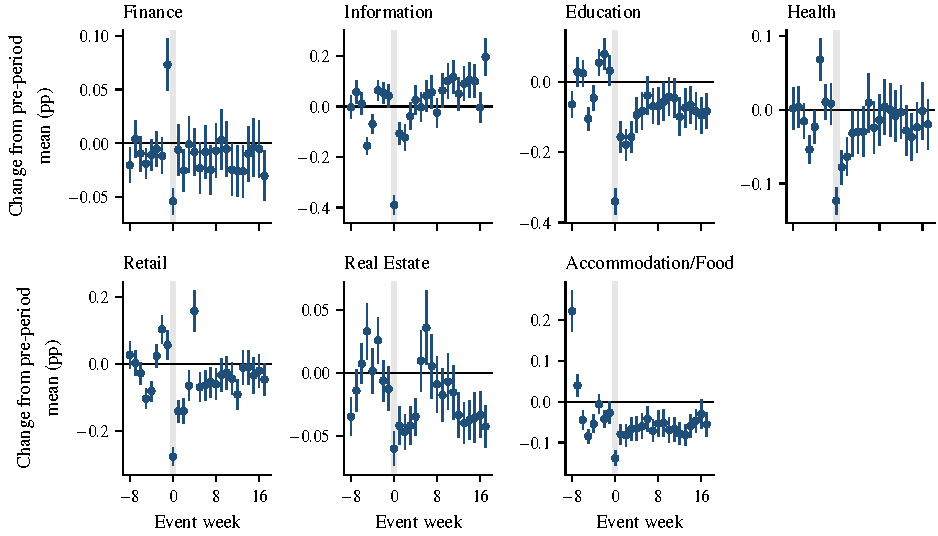
\includegraphics[width=\textwidth]{fig6_sector_eventstudy.pdf}
\fignote{Points are $\beta_{sk}$ from \cref{eq:sector}: the mean change, across the fixed sample of 20,000 Bangladesh-associated accounts, in the daily probability of a PushEvent in a sector-$s$ repository during event week $k$, relative to each user's mean over May 23--July 17, 2024, in percentage points. Vertical lines are 95 percent confidence intervals from the cross-user standard deviation of these differences; they capture sampling variation across users but not common weekly shocks. Shaded: July 18--23 shutdown; the window ends at week $+17$ (November 13--19). Vertical scales differ across panels. Within-Bangladesh descriptive comparison, not a causal effect relative to an untreated control. Source: Author's calculations using GH Archive.}
\end{figure}

% Generated by analysis/tables/make_all_tables.py -- do not edit by hand.
\begin{table}[H]
\centering
\footnotesize
\caption{Sectoral recovery indices by classifier-confidence threshold}
\label{tab:sector_threshold}
\begin{threeparttable}
\begin{tabular}{llrrrrr}
\toprule
Sector & Threshold & Pre users & Week +1 & Week +4 & Week +8 & First wk $\geq$80, 2 wks \\
\midrule
Finance & 0.70 & 437 & 91.6 & 92.4 & 89.2 & 3 \\
 & 0.80 & 382 & 92.2 & 89.5 & 91.3 & 3 \\
 & 0.90 & 275 & 101.7 & 82.5 & 101.7 & 3 \\
Information & 0.70 & 2,123 & 73.0 & 116.6 & 101.3 & 3 \\
 & 0.80 & 1,528 & 75.9 & 106.0 & 94.5 & 3 \\
 & 0.90 & 968 & 79.5 & 97.6 & 91.5 & 3 \\
Education & 0.70 & 1,345 & 61.6 & 75.4 & 79.4 & 5 \\
 & 0.80 & 1,234 & 59.1 & 75.4 & 81.9 & 6 \\
 & 0.90 & 1,029 & 57.8 & 73.3 & 77.0 & 6 \\
Health & 0.70 & 542 & 40.8 & 76.4 & 88.3 & 6 \\
 & 0.80 & 514 & 40.7 & 77.5 & 89.4 & 6 \\
 & 0.90 & 455 & 41.1 & 75.5 & 87.6 & 8 \\
Retail & 0.70 & 1,090 & 52.2 & 159.1 & 82.5 & 4 \\
 & 0.80 & 1,012 & 52.0 & 153.7 & 79.6 & 9 \\
 & 0.90 & 829 & 50.1 & 157.4 & 80.9 & 7 \\
Real Estate & 0.70 & 228 & 33.1 & 45.5 & 90.0 & 5 \\
 & 0.80 & 213 & 33.0 & 44.4 & 85.5 & 5 \\
 & 0.90 & 153 & 44.9 & 44.9 & 75.5 & 5 \\
Accommodation/Food & 0.70 & 514 & 46.0 & 59.3 & 64.9 & -- \\
 & 0.80 & 480 & 44.3 & 54.2 & 62.6 & -- \\
 & 0.90 & 394 & 39.2 & 45.1 & 60.3 & -- \\
\midrule \multicolumn{7}{l}{\textit{Excluded from the main figures and table}} \\
Professional/Scientific & 0.70 & 1,241 & 57.9 & 66.9 & 91.2 & 7 \\
 & 0.80 & 577 & 64.9 & 64.9 & 91.0 & 7 \\
 & 0.90 & 125 & 94.4 & 65.6 & 78.7 & 1 \\
Admin. Support & 0.70 & 268 & 30.8 & 83.0 & 77.0 & 9 \\
 & 0.80 & 196 & 32.2 & 72.9 & 84.7 & 10 \\
 & 0.90 & 48 & 5.2 & 61.9 & 56.8 & -- \\
\bottomrule
\end{tabular}
\begin{tablenotes}[flushleft]
\footnotesize\raggedright
\item \textit{Notes:} Each row repeats the main specification (\cref{tab:sector_recovery}) keeping only repositories whose classifier confidence is at least the stated threshold; 0.80 is the main specification. Professional/Scientific and Administrative Support are excluded from the main results because their support falls sharply at the 0.90 threshold. Source: \texttt{results/sector\_recovery/final/sector\_threshold\_robustness\_full.csv}.
\end{tablenotes}
\end{threeparttable}
\end{table}

% Generated by analysis/tables/make_all_tables.py -- do not edit by hand.
\begin{table}[H]
\centering
\footnotesize
\caption{Recovery of pre-existing repositories versus sector-wide user activity}
\label{tab:sector_fixed_repo}
\begin{threeparttable}
\begin{tabular}{lrrrrrrr}
\toprule
& & \multicolumn{3}{c}{Fixed pre-period repositories} & \multicolumn{3}{c}{Sector-wide (main)} \\
\cmidrule(lr){3-5}\cmidrule(lr){6-8}
Sector & Repos & +1 & +4 & +8 & +1 & +4 & +8 \\
\midrule
Finance & 417 & 60.0 & 28.3 & 23.0 & 92.2 & 89.5 & 91.3 \\
Information & 2,040 & 46.8 & 37.4 & 27.3 & 75.9 & 106.0 & 94.5 \\
Education & 1,523 & 40.3 & 38.2 & 31.4 & 59.1 & 75.4 & 81.9 \\
Health & 651 & 25.1 & 28.6 & 23.1 & 40.7 & 77.5 & 89.4 \\
Retail & 1,322 & 28.7 & 30.9 & 19.8 & 52.0 & 153.7 & 79.6 \\
Real Estate & 254 & 16.1 & 25.7 & 30.0 & 33.0 & 44.4 & 85.5 \\
Accommodation/Food & 581 & 29.4 & 16.1 & 10.1 & 44.3 & 54.2 & 62.6 \\
\bottomrule
\end{tabular}
\begin{tablenotes}[flushleft]
\footnotesize\raggedright
\item \textit{Notes:} Recovery indices (pre-period mean = 100). \textit{Fixed pre-period repositories}: classified repositories (confidence $\geq$ 0.80) with at least one PushEvent by a sampled user during the final eight pre-shutdown weeks; the outcome is each repository's daily PushEvent active-day rate, and new repositories never enter. \textit{Sector-wide}: main specification of \cref{tab:sector_recovery}, which includes activity on repositories first observed after the shutdown. Because a cohort selected on recent activity would decline over time even without a shutdown, the fixed-repository indices are not a counterfactual for the sector-wide indices. Sources: \texttt{results/sector\_recovery/pre8/sector\_recovery\_summary\_pre8.csv} and \texttt{results/sector\_recovery/sectorwide/sectorwide\_recovery\_summary.csv}.
\end{tablenotes}
\end{threeparttable}
\end{table}


\clearpage
\subsection{Connectivity chronology and threats to the comparison}
\label{app:connectivity_audit}

The connectivity record is useful both for defining exposure and for assessing the comparison series. Network traffic is not itself a measure of GitHub production, and a provider-level disruption need not affect every account in a country. The following review records documented events within the May 1--September 4 observation period. Absence from these non-exhaustive reports is not evidence of uninterrupted connectivity.

\begin{table}[htbp]
\centering\small
\caption{Documented connectivity events relevant to the analysis}
\label{tab:evidence_connectivity}
\begin{threeparttable}
\begin{tabular}{@{}p{.14\textwidth}p{.16\textwidth}p{.36\textwidth}p{.25\textwidth}@{}}
\toprule
Country & Date (2024) & Documented event & Implication \\
\midrule
Bangladesh & July 18 & Near-zero national traffic around 15:00 UTC \citep{belson2024} & Daily July 18 includes pre-cut hours. \\
Bangladesh & July 23 & Broadband recovery at 13:00 UTC in the August report, 12:00 UTC in Q3 \citep{belson2024,belson2024q3} & Both endpoints retained in author-cohort counts. \\
Bangladesh & July 28 & Major mobile networks recover around 09:00 UTC \citep{belson2024} & Restoration differs across access networks. \\
Bangladesh & August 4--5 & Renewed mobile outage, followed by national interruption on August 5 \citep{belson2024q3} & Later dip has additional network exposure. \\
Kenya & May 2; May 12 & Power-related disruption; submarine-cable failures \citep{cloudflare2024} & Pre-period donor contamination. \\
Kenya & June 25 & Large traffic disruption during protests; cause disputed \citep{cloudflare2024} & Connectivity and unrest are not separated. \\
Kenya & August 30--31 & Power-outage disruption \citep{belson2024q3} & Later synthetic path may be depressed. \\
Pakistan & July 31 & About two hours of disruption, with roughly 45\% national traffic decline \citep{belson2024} & Outside primary window; affects recovery comparison. \\
Nepal & May 2; June 3 & Provider outages associated with upstream payments and routing \citep{cloudflare2024} & Exposure differs by provider. \\
Malaysia & May 21 & Celcom disruption; a separate apparent dip was a Cloudflare processing issue \citep{cloudflare2024} & Telemetry artefacts must not be coded as outages. \\
\bottomrule\end{tabular}
\begin{tablenotes}[flushleft]\footnotesize
\item Times are UTC. This source audit does not change the donor pool or refit weights. Pakistan's regional July restrictions are discussed in the main donor diagnostics. The August 6 reopening reported by BSS conflicts with August 6--7 holiday labels in the input panel; the original labels and separate sensitivity remain documented. Kenya and Pakistan have positive national weights, so their post-window disruptions are especially relevant to apparent catch-up. No causal GitHub effect is assigned to a listed event solely because it appears in the chronology.
\end{tablenotes}\end{threeparttable}
\end{table}

\clearpage
\subsection{Detailed residual-publication audit}
\label{app:residual_audit}

\begin{table}[htbp]
\centering\small
\caption{Pre-period activity and the automation component of residual publication}
\label{tab:evidence_features}
\begin{threeparttable}
\begin{tabular}{@{}p{0.38\textwidth}rrrr@{}}
\toprule
Group & Users & Active days (\%) & Pushes & Fri--Sat (\%) \\
\midrule
All eligible & 10,241 & 17.25 & 21.0 & 25.96 \\
Core publishers & 40 & 36.76 & 47.5 & 24.08 \\
Core with automated heads & 18 & 52.35 & 79.5 & 23.11 \\
Other core publishers & 22 & 24.01 & 20.5 & 24.88 \\
Other eligible users & 10,201 & 17.18 & 21.0 & 25.97 \\
Onset authors & 250 & 32.62 & 51.5 & 24.59 \\
\bottomrule\end{tabular}
\begin{tablenotes}[flushleft]\footnotesize
\item May 1--July 17. Active days is the mean percentage of the 78 days; pushes is the median count. Fri--Sat is the mean account-level share of active days falling on Bangladesh's Friday--Saturday weekend (using UTC day labels), conditional on at least one active day. Grouping by automated heads concerns observed July 19--22 activity, not account type. Onset authors overlap with other groups. No causal or occupational interpretation is implied.
\end{tablenotes}\end{threeparttable}\end{table}


\begin{figure}[htbp]
\centering
\caption{Core-window pushes by strength of automation evidence}
\label{fig:evidence_automation}
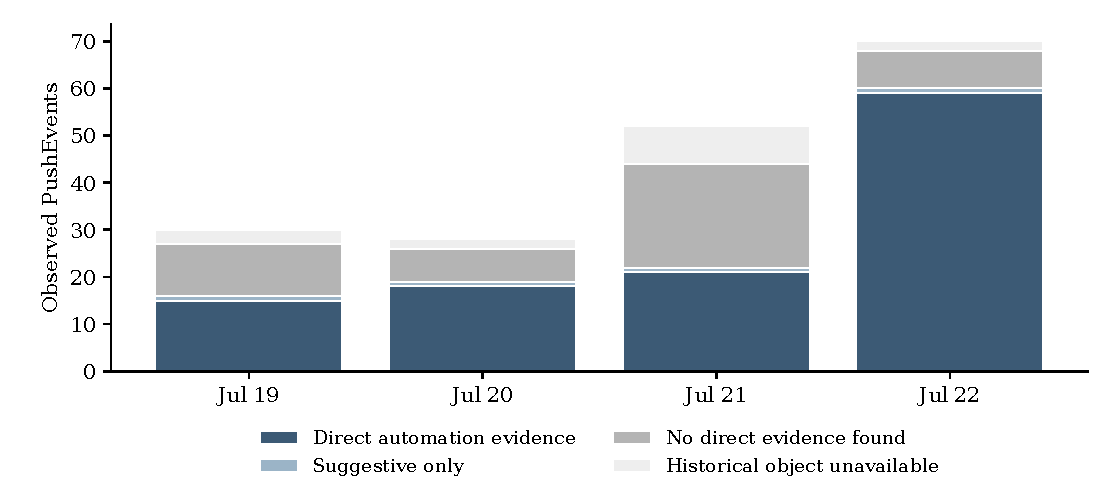
\includegraphics[width=\textwidth]{fig_evidence_automation.pdf}
\fignote{All 180 PushEvents on July 19--22 from the 40 core publishers. Classification concerns the head commit and available historical evidence. Direct evidence requires a machine identity corroborated by messages/files or a matching generating workflow; suggestive patterns and unavailable objects remain separate. No-direct-evidence cases are not certified human activity. Non-push primary events are omitted from this figure but retained in Table~\ref{tab:evidence_audit}.}
\end{figure}

\clearpage
{\footnotesize\setlength{\tabcolsep}{3pt}
\begin{longtable}{@{}p{.065\textwidth}rrp{.13\textwidth}p{.61\textwidth}@{}}
\caption{Individual review of every core-window publisher}\label{tab:evidence_cases}\\
\toprule Case & Events & Auto & Evidence & Basis and qualification \\
\midrule\endfirsthead
\toprule Case & Events & Auto & Evidence & Basis and qualification \\
\midrule\endhead
\bottomrule\endfoot
C002 & 4 & 4 & Direct & GitHub Actions author; generated snake SVG files. \\
C003 & 4 & 4 & Direct & readme-bot; scheduled WakaTime README workflow. \\
C006 & 1 & 0 & Not identified & Kubernetes/project files; no identified automated publishing mechanism. \\
C008 & 3 & 3 & Direct & readme-bot; historical scheduled WakaTime workflow. \\
C014 & 5 & 0 & Not identified & Build-fix commits; CI and stale-issue workflows do not establish automation of these pushes. \\
C021 & 5 & 0 & Not identified & IDE-file removals and a project README; no direct automation evidence. \\
C024 & 8 & 0 & Insufficient & Eight regularly timed profile-repository pushes, but historical objects unavailable; timing alone is insufficient. \\
C039 & 21 & 7 & Direct & Snyk bot heads; dependency-upgrade messages and manifests. \\
C043 & 16 & 16 & Direct & GitHub Actions author; generated snake SVG files. \\
C047 & 3 & 0 & Not identified & Favicon and application changes; no identified automatic publisher. \\
C049 & 10 & 0 & Not identified & Stack/queue exercises and React signup edits; repetitive messages alone do not establish automation. \\
C051 & 3 & 3 & Direct & readme-bot; historical scheduled WakaTime workflow. \\
C062 & 3 & 1 & Direct & Snyk bot head; lucide-react dependency upgrade. \\
C070 & 4 & 4 & Direct & github-actions identity; scheduled video-index pipeline and matching commit message. \\
C083 & 4 & 0 & Suggestive & Four 22:00 UTC host-list updates; an update-and-push script and example crontab exist, but deployment of that schedule is unverified. \\
C084 & 8 & 8 & Direct & github-actions[bot] author; generated deployment output, not inferred from the repository topic. \\
C089 & 4 & 4 & Direct & readme-bot; historical scheduled WakaTime workflow. \\
C093 & 6 & 2 & Direct & Snyk bot heads; mysql2 dependency upgrades. \\
C098 & 1 & 0 & Not identified & Engineering scripts/documents; no identified automatic publisher; commit title uses a local calendar date. \\
C099 & 3 & 0 & Not identified & HTML/CSS fitness-layout edits; no identified automatic publisher. \\
C110 & 2 & 1 & Direct & pyup-bot identity; Sphinx dependency update. \\
C115 & 3 & 1 & Direct & Snyk bot head; dependency-upgrade manifest changes. \\
C116 & 2 & 0 & Not identified & Application project-page edits; no identified automatic publisher. \\
C119 & 2 & 0 & Insufficient & Two CreateEvents only; no commit to inspect. Repository creation is not evidence of coding. \\
C123 & 1 & 0 & Not identified & Java generic-type examples; no identified automatic publisher. \\
C133 & 1 & 0 & Not identified & Three-line HTML change through GitHub UI; GitHub/web-flow is not itself bot evidence. \\
C139 & 7 & 0 & Not identified & Authentication and interface changes; no identified automatic publisher. \\
C140 & 4 & 0 & Mixed & Mixed activity: BibTeX edits and a merge; one onset commit is generated by github-actions[bot] and an exact historical import workflow. \\
C148 & 1 & 0 & Not identified & Power-system code repository; inspected core head resolves a gitignore conflict, not an automatic release. \\
C159 & 1 & 1 & Direct & readme-bot; historical weekly WakaTime workflow. \\
C161 & 7 & 7 & Direct & GitHub Actions author; generated snake SVG files. \\
C177 & 5 & 0 & Insufficient & Historical repository and four core heads unavailable. \\
C183 & 6 & 2 & Direct & Snyk bot heads; Dockerfile vulnerability-fix updates. \\
C222 & 10 & 0 & Not identified & C-sharp interview/data-structure exercises; the term Auto Stack is not evidence of a bot. \\
C226 & 1 & 0 & Not identified & README edits via GitHub UI; no identified automatic publisher. \\
C229 & 1 & 0 & Not identified & React router and page components; no identified automatic publisher. \\
C242 & 4 & 4 & Direct & GitHub Actions author; generated snake SVG files. \\
C260 & 12 & 0 & Not identified & Kotlin multiplatform examples; repeated init messages cover different files and do not establish automation. \\
C272 & 9 & 0 & Insufficient & Three core heads in two repositories unavailable; event combinations alone are insufficient. \\
C273 & 42 & 41 & Direct & All 41 core heads identify pyup-bot and change dependency requirements. \\
\end{longtable}}
\noindent\footnotesize Events counts all primary events on July 19--22; Auto counts only directly evidenced automated push heads. ``Not identified'' is not proof of manual authorship. Mixed denotes the account with a generated onset-authored commit alongside other activity; that generated commit is not itself a core push head. Case IDs map to account/repository/commit URLs and dated API evidence in \texttt{results/evidence\_20261020/individual\_case\_review.csv}. The review is AI-assisted and has not been independently validated by a second reviewer.\normalsize



\clearpage
\subsection{Country-by-country activity and complete domain coverage}

\label{app:country_atlas}

The following figures show every country and every defined repository domain, including cells that do not qualify for a synthetic-control estimate. Cohorts and denominators are fixed before July 18 using the historical-text assignment described in Section~\ref{sec:international_sector_data}. A small or empty cell is shown explicitly; it is not replaced by a zero causal effect. These plots describe measured public activity and do not identify employment industries.

\begin{figure}[H]\centering

\caption{Eligible accounts by country and pre-treatment repository domain}

\label{fig:country_domain_support}

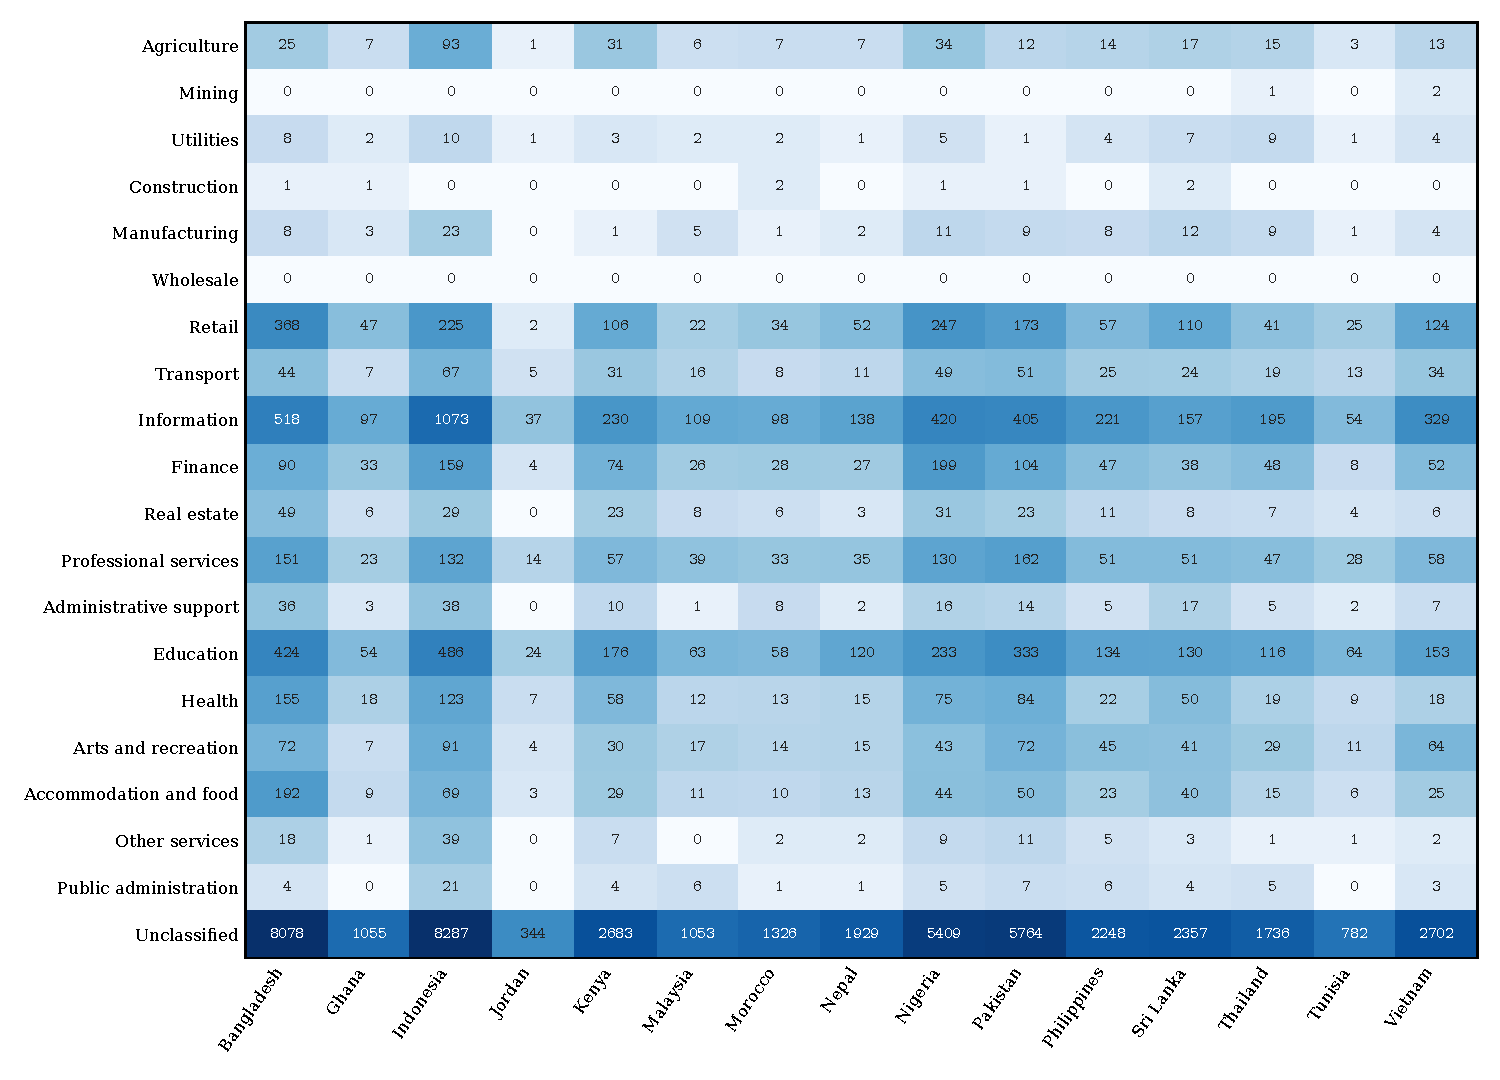
\includegraphics[width=\textwidth]{fig_evidence_country_domain_support.pdf}

\fignote{Numbers are fixed cohort sizes. Colour represents $\log_{10}(1+N)$ for readability. All 59,158 eligible users are assigned exactly once, including the unclassified group. The existing estimation screen requires at least 30 Bangladesh users and five donor countries with at least 30 users each; these descriptive figures apply no such deletion.}

\end{figure}\clearpage

\begin{figure}[p]\centering

\caption{Daily public activity in Bangladesh and every donor country}

\label{fig:country_national}

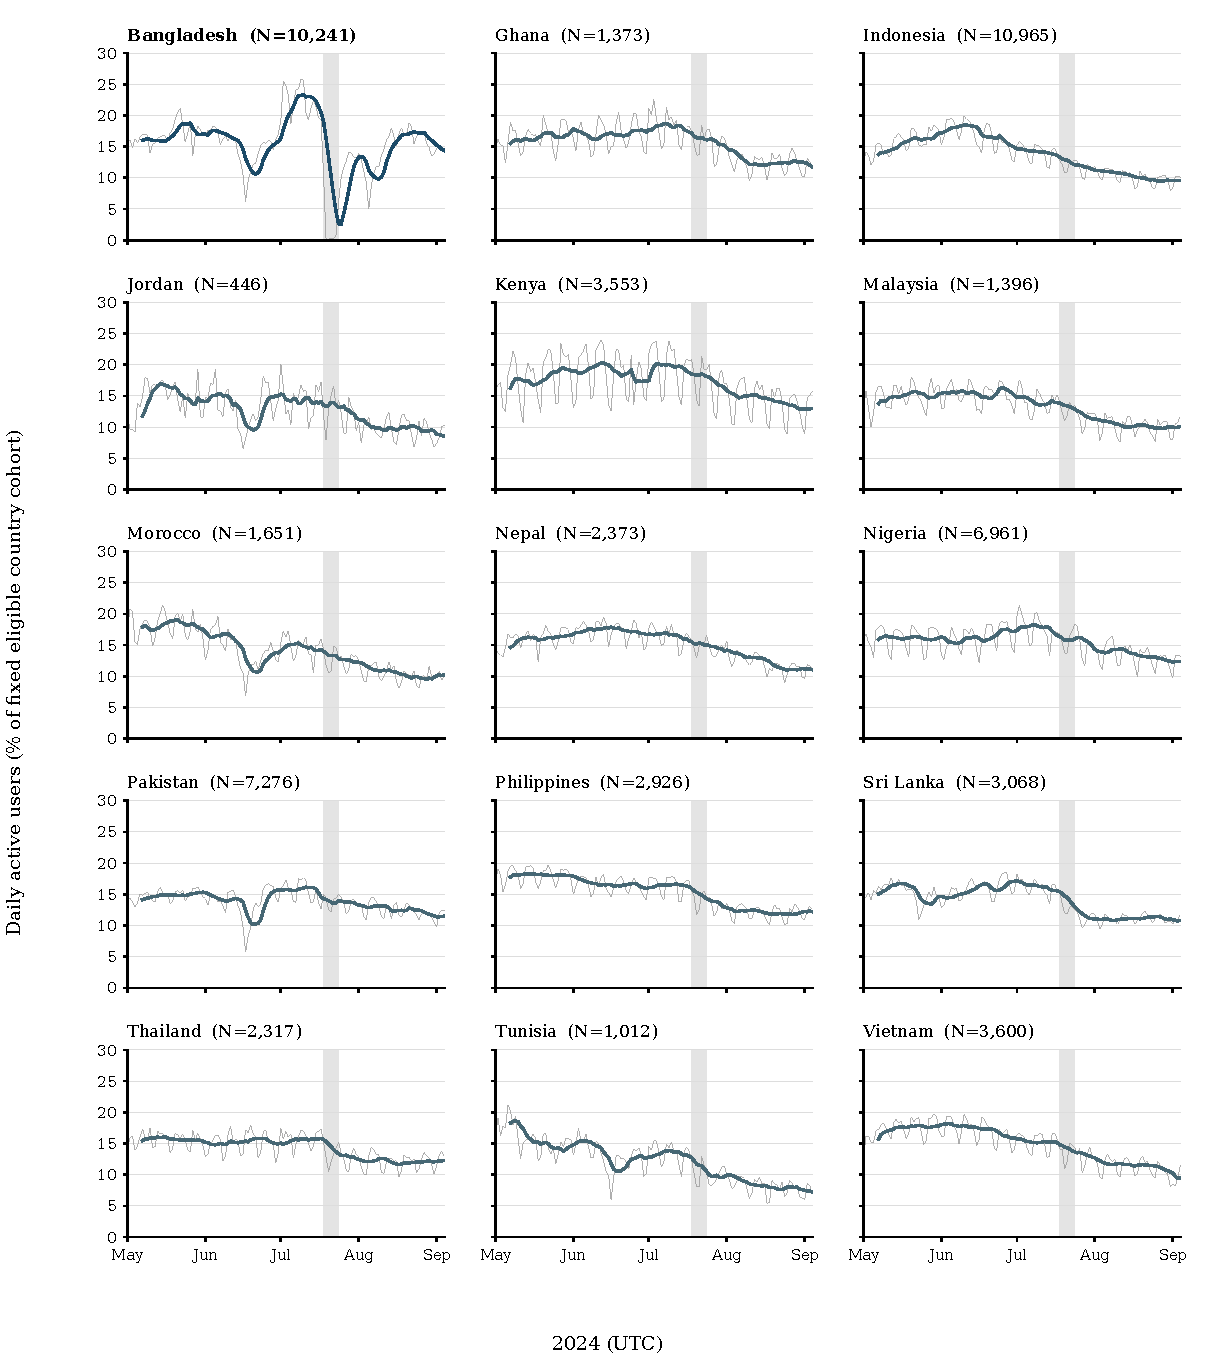
\includegraphics[width=\textwidth,height=.81\textheight,keepaspectratio]{fig_evidence_country_national.pdf}

\fignote{Thin grey lines: daily rates; coloured lines: trailing seven-day means, shown only after seven observations. Grey shading: July 18--23. All days and rates use UTC and the original country denominators. The smoothing is descriptive and is not used to re-estimate the primary model.}

\end{figure}\clearpage

\begin{figure}[p]\centering

\caption{Country-by-country public activity: Agriculture}

\label{fig:atlas_11}

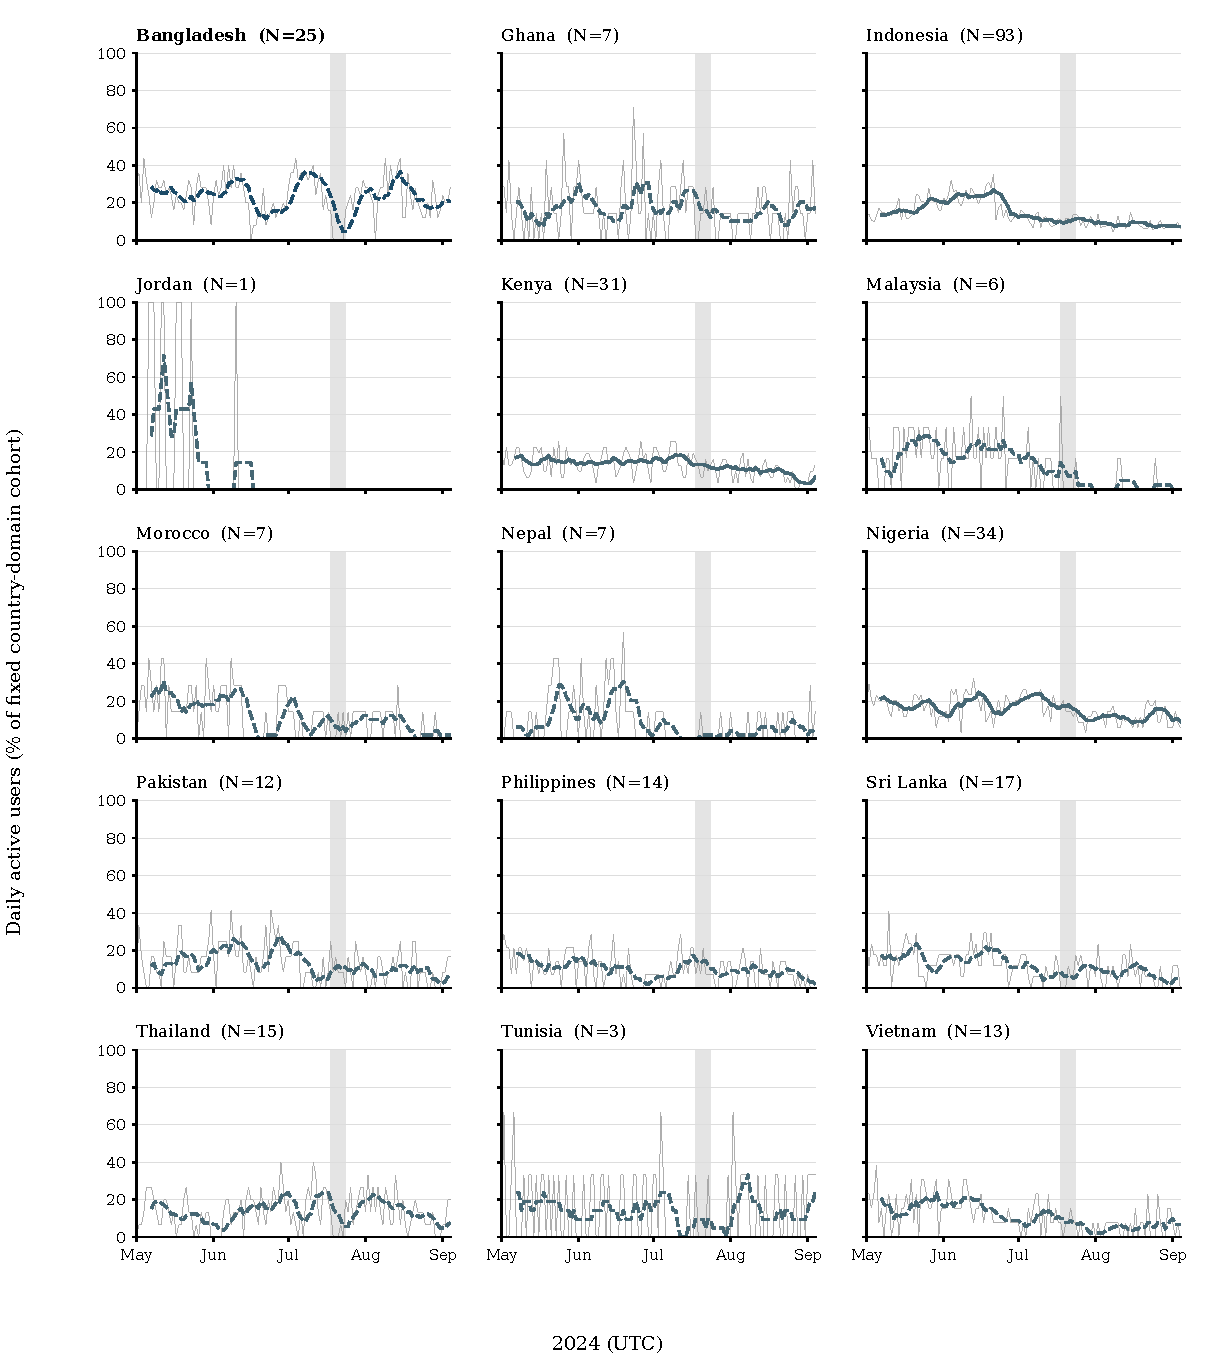
\includegraphics[page=1,width=\textwidth,height=.81\textheight,keepaspectratio]{fig_evidence_country_sectors.pdf}

\fignote{Fixed historical-README cohort, confidence threshold 0.80. Thin grey: daily rates; coloured: trailing seven-day mean. Dashed means indicate fewer than 30 users; empty cells have no assigned users. Scales are common across countries on this page but may differ across domains. Grey shading: July 18--23. The outcome counts each assigned user's primary activity anywhere on GitHub, not only activity in the repository used for assignment.}

\end{figure}\clearpage

\begin{figure}[p]\centering

\caption{Country-by-country public activity: Mining}

\label{fig:atlas_21}

\includegraphics[page=2,width=\textwidth,height=.81\textheight,keepaspectratio]{fig_evidence_country_sectors.pdf}

\fignote{Fixed historical-README cohort, confidence threshold 0.80. Thin grey: daily rates; coloured: trailing seven-day mean. Dashed means indicate fewer than 30 users; empty cells have no assigned users. Scales are common across countries on this page but may differ across domains. Grey shading: July 18--23. The outcome counts each assigned user's primary activity anywhere on GitHub, not only activity in the repository used for assignment.}

\end{figure}\clearpage

\begin{figure}[p]\centering

\caption{Country-by-country public activity: Utilities}

\label{fig:atlas_22}

\includegraphics[page=3,width=\textwidth,height=.81\textheight,keepaspectratio]{fig_evidence_country_sectors.pdf}

\fignote{Fixed historical-README cohort, confidence threshold 0.80. Thin grey: daily rates; coloured: trailing seven-day mean. Dashed means indicate fewer than 30 users; empty cells have no assigned users. Scales are common across countries on this page but may differ across domains. Grey shading: July 18--23. The outcome counts each assigned user's primary activity anywhere on GitHub, not only activity in the repository used for assignment.}

\end{figure}\clearpage

\begin{figure}[p]\centering

\caption{Country-by-country public activity: Construction}

\label{fig:atlas_23}

\includegraphics[page=4,width=\textwidth,height=.81\textheight,keepaspectratio]{fig_evidence_country_sectors.pdf}

\fignote{Fixed historical-README cohort, confidence threshold 0.80. Thin grey: daily rates; coloured: trailing seven-day mean. Dashed means indicate fewer than 30 users; empty cells have no assigned users. Scales are common across countries on this page but may differ across domains. Grey shading: July 18--23. The outcome counts each assigned user's primary activity anywhere on GitHub, not only activity in the repository used for assignment.}

\end{figure}\clearpage

\begin{figure}[p]\centering

\caption{Country-by-country public activity: Manufacturing}

\label{fig:atlas_31-33}

\includegraphics[page=5,width=\textwidth,height=.81\textheight,keepaspectratio]{fig_evidence_country_sectors.pdf}

\fignote{Fixed historical-README cohort, confidence threshold 0.80. Thin grey: daily rates; coloured: trailing seven-day mean. Dashed means indicate fewer than 30 users; empty cells have no assigned users. Scales are common across countries on this page but may differ across domains. Grey shading: July 18--23. The outcome counts each assigned user's primary activity anywhere on GitHub, not only activity in the repository used for assignment.}

\end{figure}\clearpage

\begin{figure}[p]\centering

\caption{Country-by-country public activity: Wholesale}

\label{fig:atlas_42}

\includegraphics[page=6,width=\textwidth,height=.81\textheight,keepaspectratio]{fig_evidence_country_sectors.pdf}

\fignote{Fixed historical-README cohort, confidence threshold 0.80. Thin grey: daily rates; coloured: trailing seven-day mean. Dashed means indicate fewer than 30 users; empty cells have no assigned users. Scales are common across countries on this page but may differ across domains. Grey shading: July 18--23. The outcome counts each assigned user's primary activity anywhere on GitHub, not only activity in the repository used for assignment.}

\end{figure}\clearpage

\begin{figure}[p]\centering

\caption{Country-by-country public activity: Retail}

\label{fig:atlas_44-45}

\includegraphics[page=7,width=\textwidth,height=.81\textheight,keepaspectratio]{fig_evidence_country_sectors.pdf}

\fignote{Fixed historical-README cohort, confidence threshold 0.80. Thin grey: daily rates; coloured: trailing seven-day mean. Dashed means indicate fewer than 30 users; empty cells have no assigned users. Scales are common across countries on this page but may differ across domains. Grey shading: July 18--23. The outcome counts each assigned user's primary activity anywhere on GitHub, not only activity in the repository used for assignment.}

\end{figure}\clearpage

\begin{figure}[p]\centering

\caption{Country-by-country public activity: Transport}

\label{fig:atlas_48-49}

\includegraphics[page=8,width=\textwidth,height=.81\textheight,keepaspectratio]{fig_evidence_country_sectors.pdf}

\fignote{Fixed historical-README cohort, confidence threshold 0.80. Thin grey: daily rates; coloured: trailing seven-day mean. Dashed means indicate fewer than 30 users; empty cells have no assigned users. Scales are common across countries on this page but may differ across domains. Grey shading: July 18--23. The outcome counts each assigned user's primary activity anywhere on GitHub, not only activity in the repository used for assignment.}

\end{figure}\clearpage

\begin{figure}[p]\centering

\caption{Country-by-country public activity: Information}

\label{fig:atlas_51}

\includegraphics[page=9,width=\textwidth,height=.81\textheight,keepaspectratio]{fig_evidence_country_sectors.pdf}

\fignote{Fixed historical-README cohort, confidence threshold 0.80. Thin grey: daily rates; coloured: trailing seven-day mean. Dashed means indicate fewer than 30 users; empty cells have no assigned users. Scales are common across countries on this page but may differ across domains. Grey shading: July 18--23. The outcome counts each assigned user's primary activity anywhere on GitHub, not only activity in the repository used for assignment.}

\end{figure}\clearpage

\begin{figure}[p]\centering

\caption{Country-by-country public activity: Finance}

\label{fig:atlas_52}

\includegraphics[page=10,width=\textwidth,height=.81\textheight,keepaspectratio]{fig_evidence_country_sectors.pdf}

\fignote{Fixed historical-README cohort, confidence threshold 0.80. Thin grey: daily rates; coloured: trailing seven-day mean. Dashed means indicate fewer than 30 users; empty cells have no assigned users. Scales are common across countries on this page but may differ across domains. Grey shading: July 18--23. The outcome counts each assigned user's primary activity anywhere on GitHub, not only activity in the repository used for assignment.}

\end{figure}\clearpage

\begin{figure}[p]\centering

\caption{Country-by-country public activity: Real estate}

\label{fig:atlas_53}

\includegraphics[page=11,width=\textwidth,height=.81\textheight,keepaspectratio]{fig_evidence_country_sectors.pdf}

\fignote{Fixed historical-README cohort, confidence threshold 0.80. Thin grey: daily rates; coloured: trailing seven-day mean. Dashed means indicate fewer than 30 users; empty cells have no assigned users. Scales are common across countries on this page but may differ across domains. Grey shading: July 18--23. The outcome counts each assigned user's primary activity anywhere on GitHub, not only activity in the repository used for assignment.}

\end{figure}\clearpage

\begin{figure}[p]\centering

\caption{Country-by-country public activity: Professional services}

\label{fig:atlas_54}

\includegraphics[page=12,width=\textwidth,height=.81\textheight,keepaspectratio]{fig_evidence_country_sectors.pdf}

\fignote{Fixed historical-README cohort, confidence threshold 0.80. Thin grey: daily rates; coloured: trailing seven-day mean. Dashed means indicate fewer than 30 users; empty cells have no assigned users. Scales are common across countries on this page but may differ across domains. Grey shading: July 18--23. The outcome counts each assigned user's primary activity anywhere on GitHub, not only activity in the repository used for assignment.}

\end{figure}\clearpage

\begin{figure}[p]\centering

\caption{Country-by-country public activity: Administrative support}

\label{fig:atlas_56}

\includegraphics[page=13,width=\textwidth,height=.81\textheight,keepaspectratio]{fig_evidence_country_sectors.pdf}

\fignote{Fixed historical-README cohort, confidence threshold 0.80. Thin grey: daily rates; coloured: trailing seven-day mean. Dashed means indicate fewer than 30 users; empty cells have no assigned users. Scales are common across countries on this page but may differ across domains. Grey shading: July 18--23. The outcome counts each assigned user's primary activity anywhere on GitHub, not only activity in the repository used for assignment.}

\end{figure}\clearpage

\begin{figure}[p]\centering

\caption{Country-by-country public activity: Education}

\label{fig:atlas_61}

\includegraphics[page=14,width=\textwidth,height=.81\textheight,keepaspectratio]{fig_evidence_country_sectors.pdf}

\fignote{Fixed historical-README cohort, confidence threshold 0.80. Thin grey: daily rates; coloured: trailing seven-day mean. Dashed means indicate fewer than 30 users; empty cells have no assigned users. Scales are common across countries on this page but may differ across domains. Grey shading: July 18--23. The outcome counts each assigned user's primary activity anywhere on GitHub, not only activity in the repository used for assignment.}

\end{figure}\clearpage

\begin{figure}[p]\centering

\caption{Country-by-country public activity: Health}

\label{fig:atlas_62}

\includegraphics[page=15,width=\textwidth,height=.81\textheight,keepaspectratio]{fig_evidence_country_sectors.pdf}

\fignote{Fixed historical-README cohort, confidence threshold 0.80. Thin grey: daily rates; coloured: trailing seven-day mean. Dashed means indicate fewer than 30 users; empty cells have no assigned users. Scales are common across countries on this page but may differ across domains. Grey shading: July 18--23. The outcome counts each assigned user's primary activity anywhere on GitHub, not only activity in the repository used for assignment.}

\end{figure}\clearpage

\begin{figure}[p]\centering

\caption{Country-by-country public activity: Arts and recreation}

\label{fig:atlas_71}

\includegraphics[page=16,width=\textwidth,height=.81\textheight,keepaspectratio]{fig_evidence_country_sectors.pdf}

\fignote{Fixed historical-README cohort, confidence threshold 0.80. Thin grey: daily rates; coloured: trailing seven-day mean. Dashed means indicate fewer than 30 users; empty cells have no assigned users. Scales are common across countries on this page but may differ across domains. Grey shading: July 18--23. The outcome counts each assigned user's primary activity anywhere on GitHub, not only activity in the repository used for assignment.}

\end{figure}\clearpage

\begin{figure}[p]\centering

\caption{Country-by-country public activity: Accommodation and food}

\label{fig:atlas_72}

\includegraphics[page=17,width=\textwidth,height=.81\textheight,keepaspectratio]{fig_evidence_country_sectors.pdf}

\fignote{Fixed historical-README cohort, confidence threshold 0.80. Thin grey: daily rates; coloured: trailing seven-day mean. Dashed means indicate fewer than 30 users; empty cells have no assigned users. Scales are common across countries on this page but may differ across domains. Grey shading: July 18--23. The outcome counts each assigned user's primary activity anywhere on GitHub, not only activity in the repository used for assignment.}

\end{figure}\clearpage

\begin{figure}[p]\centering

\caption{Country-by-country public activity: Other services}

\label{fig:atlas_81}

\includegraphics[page=18,width=\textwidth,height=.81\textheight,keepaspectratio]{fig_evidence_country_sectors.pdf}

\fignote{Fixed historical-README cohort, confidence threshold 0.80. Thin grey: daily rates; coloured: trailing seven-day mean. Dashed means indicate fewer than 30 users; empty cells have no assigned users. Scales are common across countries on this page but may differ across domains. Grey shading: July 18--23. The outcome counts each assigned user's primary activity anywhere on GitHub, not only activity in the repository used for assignment.}

\end{figure}\clearpage

\begin{figure}[p]\centering

\caption{Country-by-country public activity: Public administration}

\label{fig:atlas_92}

\includegraphics[page=19,width=\textwidth,height=.81\textheight,keepaspectratio]{fig_evidence_country_sectors.pdf}

\fignote{Fixed historical-README cohort, confidence threshold 0.80. Thin grey: daily rates; coloured: trailing seven-day mean. Dashed means indicate fewer than 30 users; empty cells have no assigned users. Scales are common across countries on this page but may differ across domains. Grey shading: July 18--23. The outcome counts each assigned user's primary activity anywhere on GitHub, not only activity in the repository used for assignment.}

\end{figure}\clearpage

\begin{figure}[p]\centering

\caption{Country-by-country public activity: Unclassified}

\label{fig:atlas_Unclassified}

\includegraphics[page=20,width=\textwidth,height=.81\textheight,keepaspectratio]{fig_evidence_country_sectors.pdf}

\fignote{Fixed historical-README cohort, confidence threshold 0.80. Thin grey: daily rates; coloured: trailing seven-day mean. Dashed means indicate fewer than 30 users; empty cells have no assigned users. Scales are common across countries on this page but may differ across domains. Grey shading: July 18--23. The outcome counts each assigned user's primary activity anywhere on GitHub, not only activity in the repository used for assignment.}

\end{figure}\clearpage



\end{document}
